\section*{Combustion dynamics}\label{sec:ch3_cavity_dynamics}
The combined PIV and PLIF fields may be used as complementary inputs to gain insights into the unsteady flame structure. Randomly-sampled images of the OH structures are observed throughout the dataset, which may be sorted into three main categories of state. In state 1, the flame is contained within the cavity before the ramp ($y/H<0$ and $x/H<4$). In state 2, the flame continuously extends past the cavity interface and ramp. In state 3, the extended flame is discontinuous.

The three states are consistent with the previously-stated hypothesis that thermoacoustic oscillations, due to coupling between the inlet shock-train and thermal throat, couple with combustion in the cavity \citep{WangWangSun2014, TuttleCarterHsu2014, Kirik2017, AllisonFredericksonKirikEtAl2017}.  Thermoacoustic oscillation is associated with length scales on the order of the distance between the shock train and the thermal throat. Thermoacoustic oscillation frequencies are much smaller than the frequencies of the largest cavity shear layer eddies, the freestream turbulence, and the acoustic oscillations of the cavity. Therefore, these states are not consistent with normal cavity oscillations.   The combustion cycle suggested below consists of periodic combustion product ejection through shear layer detachment from the cavity ramp. 

The present PIV-PLIF acquisition frequency of 10 Hz does not permit motions on the order of 100-1000 Hz to be resolved. However, a cyclical process may be proposed based on the identification of categories described above. Given that the combustion oscillation frequency is unlikely to be a harmonic of the PIV-PLIF acquisition frequency, one may assume that the combustion cycle is randomly captured over the available 2,000 measurements. With the additional input of the flow direction, physical inference, and the previous investigations on cavity flows listed in the introduction, the categories of instantaneous measurements may be sorted into a sequence of hypothetical states: 1-2-3.  Other orders are physically implausible. The state series 2-1-3 would imply that the extended part of the flame extinguishes before a separated flame self-ignites in the main duct flow. The state series 3-2-1 would have the separated flame self-ignite in the duct flow and propagate against the high-speed flow to connect with the upstream cavity flame.  Instantaneous measurements that illustrate these states are selected; Figs. \ref{fig:ch3_inst_B1} and \ref{fig:ch3_inst_B1vec} display velocity maps and streamlines, respectively, overlayed with an outline of the products region, as identified from PLIF. These figures also display measurements that appear to show transitions between states; these are labeled 2' (between states 2 and 3) and 3' (between states 3 and 1).  The streamlines of Fig. \ref{fig:ch3_inst_B1vec} shows that eddies are present that vary in size and location across the various states.  Figure \ref{fig:ch3_inst_ST} displays the swirling strength of vortices, which allows better localization of the strongest eddies independently of the reference frame  \citep{Adrian2000}. 

\begin{figure}
\centering
\subcaptionbox{State 1\label{fig:B1_Frame1}}
                {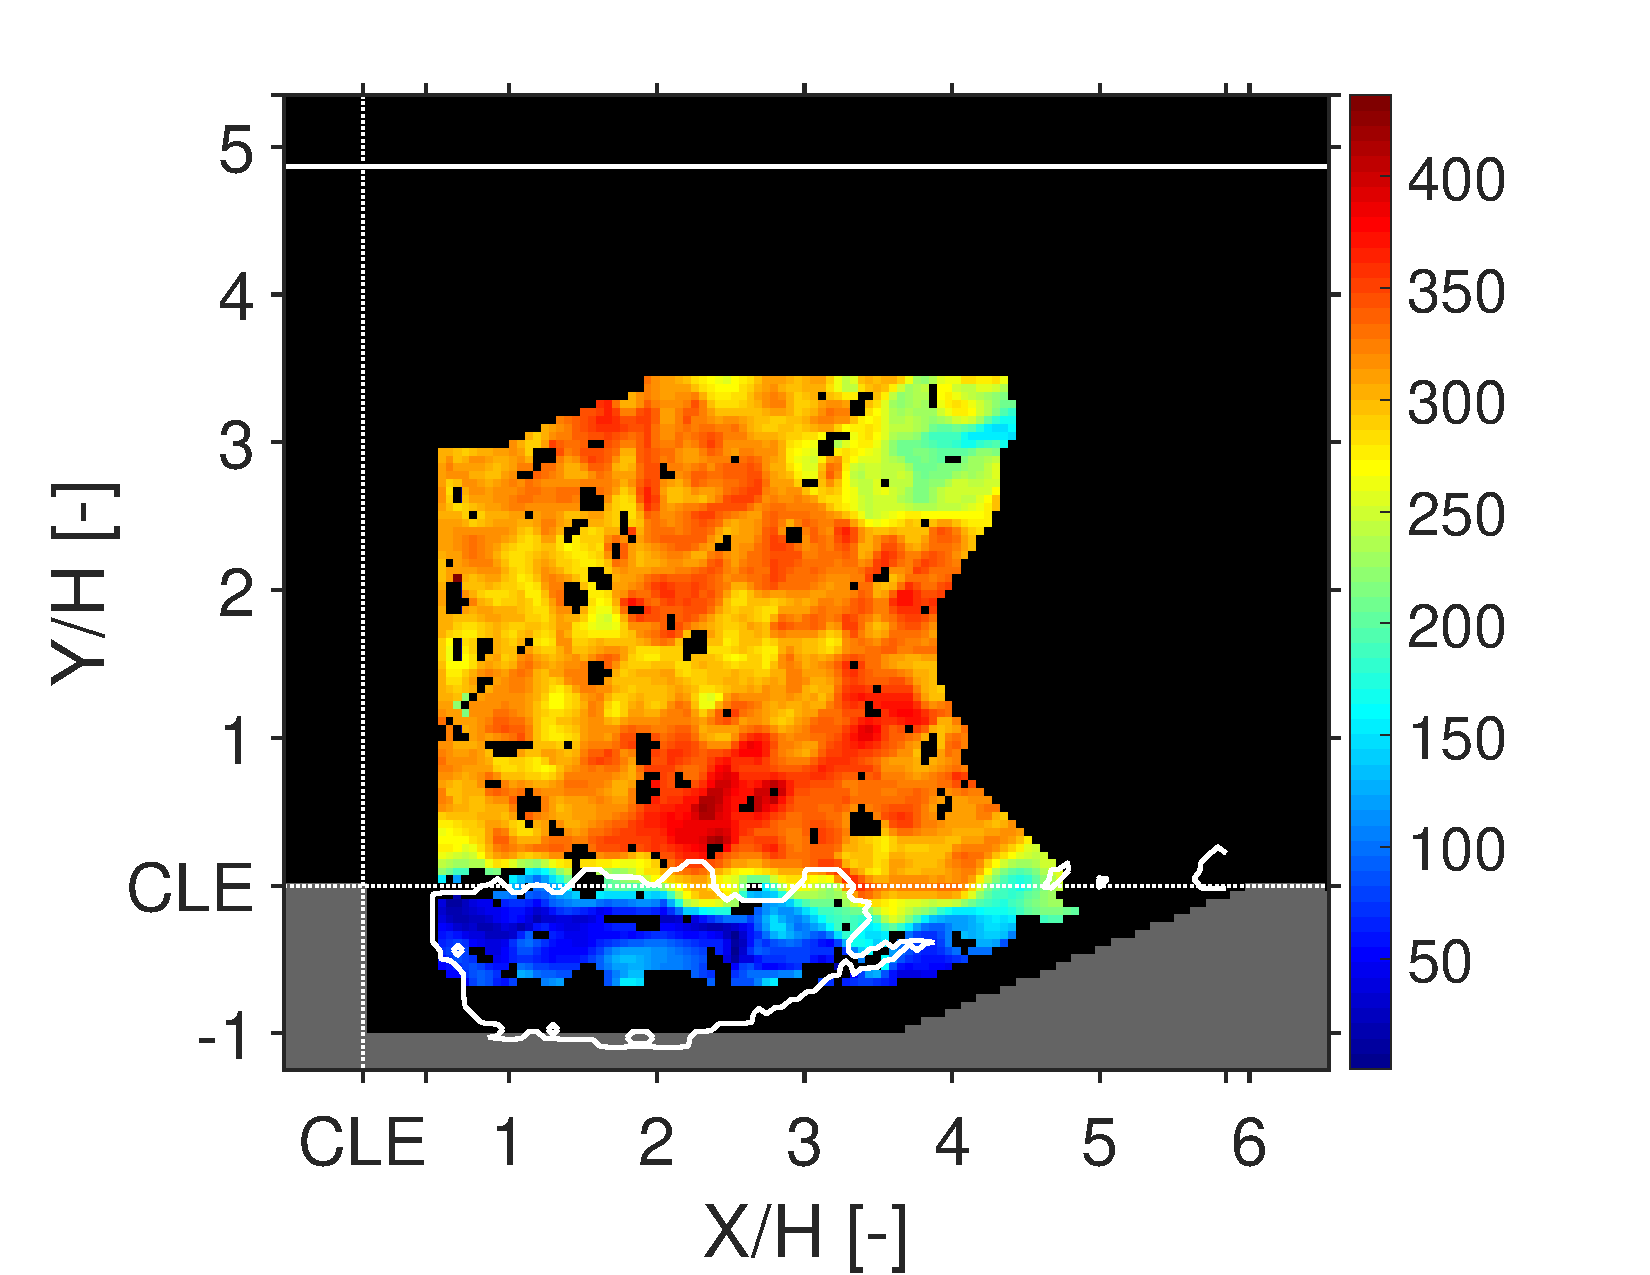
\includegraphics[width=3in,trim=0.35in 0 0.65in 0, clip]{figures/B1/combustion_instability/1/absolute_vel/B1_Frame331.pdf}\rotatebox{90}{\hspace{1.3in}\footnotesize$\mathrm{[m/s]}$}}
                \hspace{0.4cm}
\subcaptionbox{State 2\label{fig:B1_Frame2}}
                {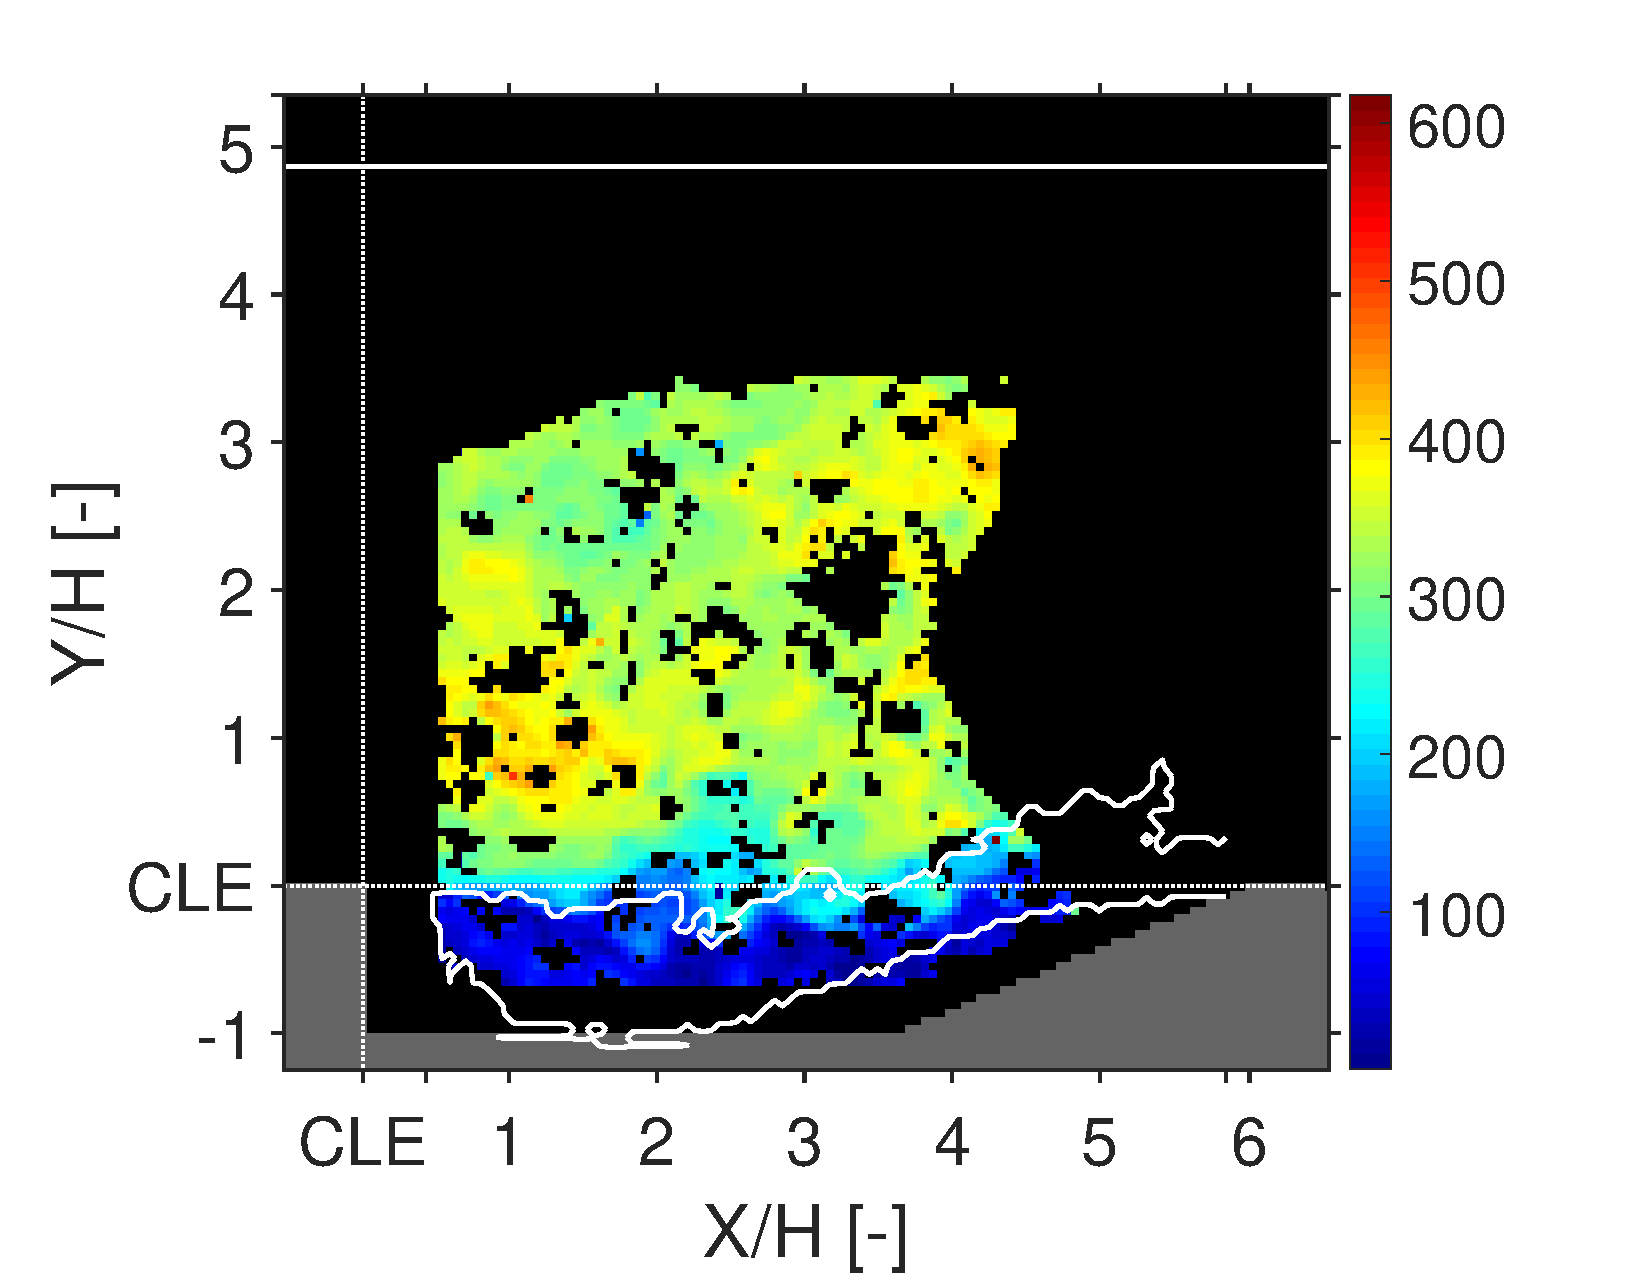
\includegraphics[width=3in,trim=0.35in 0 0.65in 0, clip]{figures/B1/combustion_instability/2/absolute_vel/B1_Frame329.pdf}\rotatebox{90}{\hspace{1.3in}\footnotesize$\mathrm{[m/s]}$}}
                \newline
\subcaptionbox{State 2'\label{fig:B1_Frame3}}
                {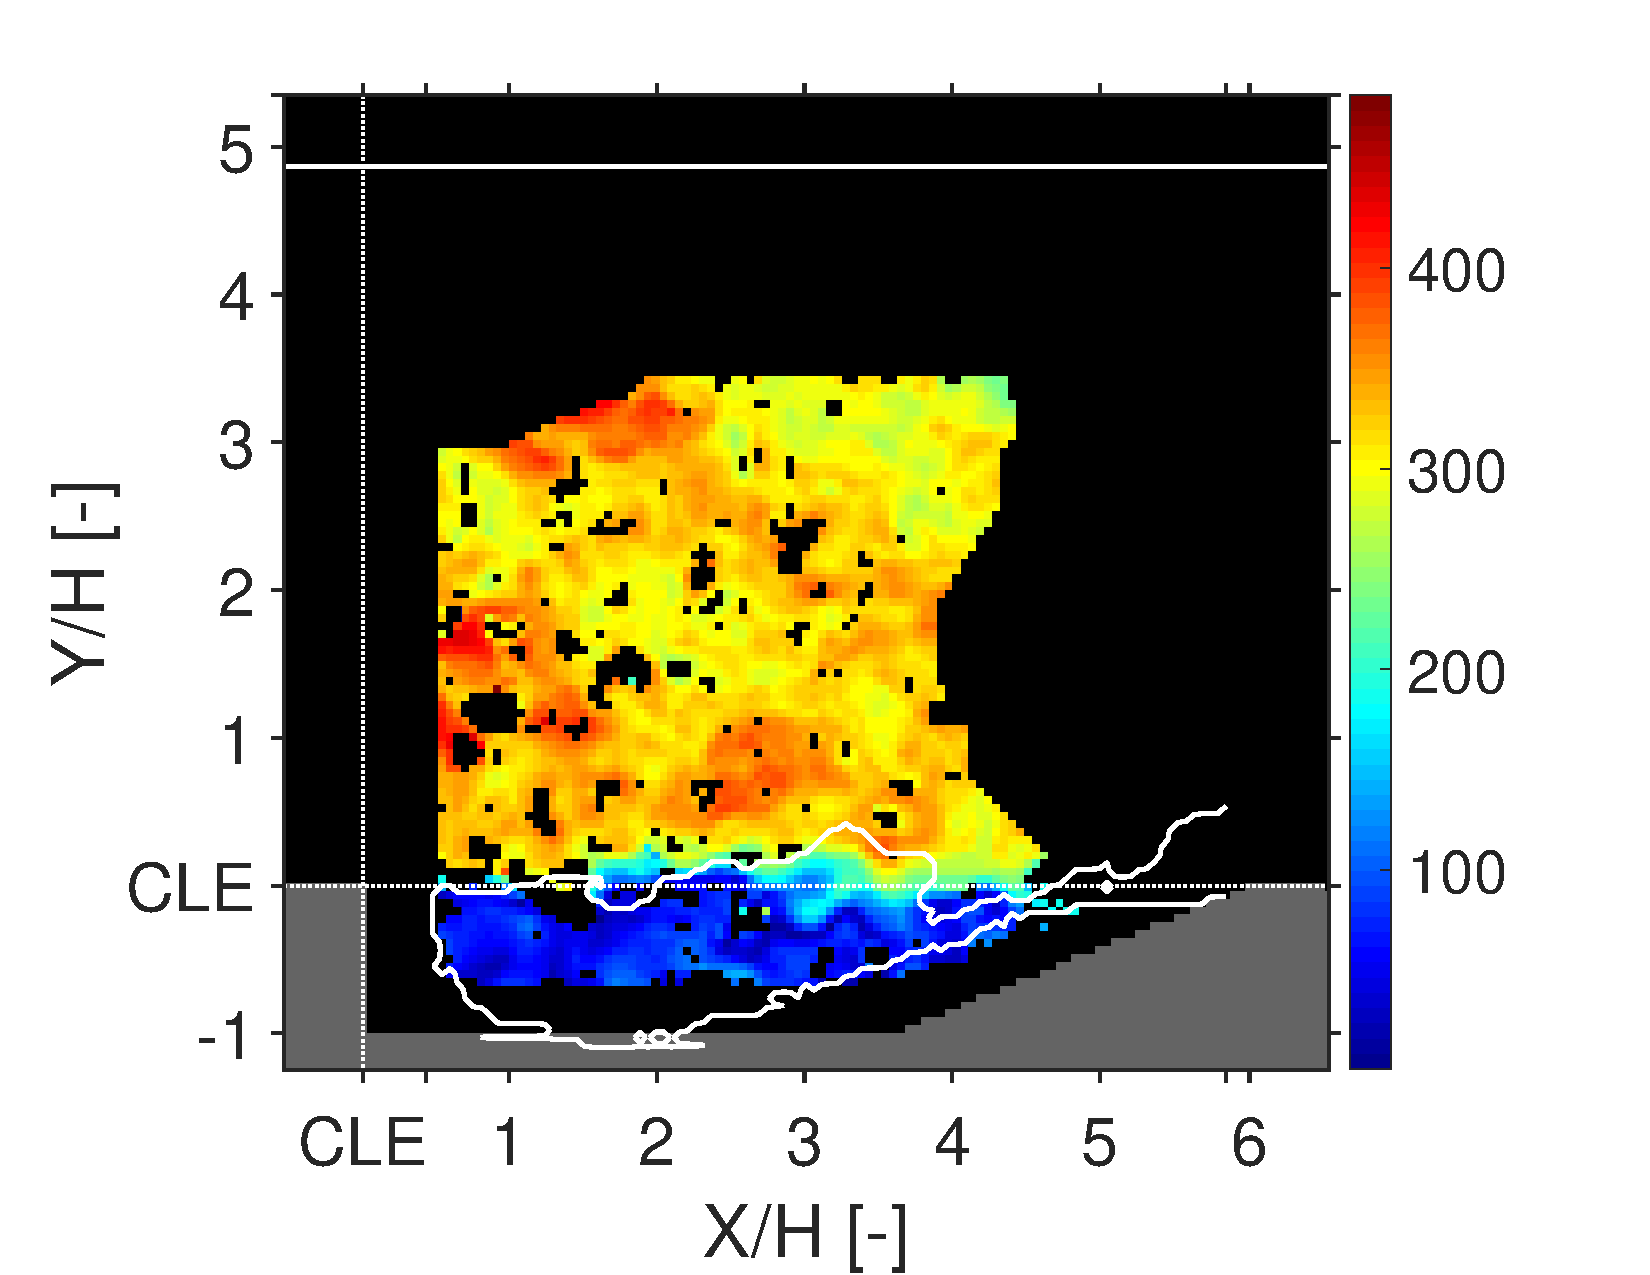
\includegraphics[width=3in,trim=0.35in 0 0.65in 0, clip]{figures/B1/combustion_instability/3/absolute_vel/B1_Frame342.pdf}\rotatebox{90}{\hspace{1.3in}\footnotesize$\mathrm{[m/s]}$}}
                \hspace{0.4cm}
\subcaptionbox{State 3\label{fig:B1_Frame4}}
                {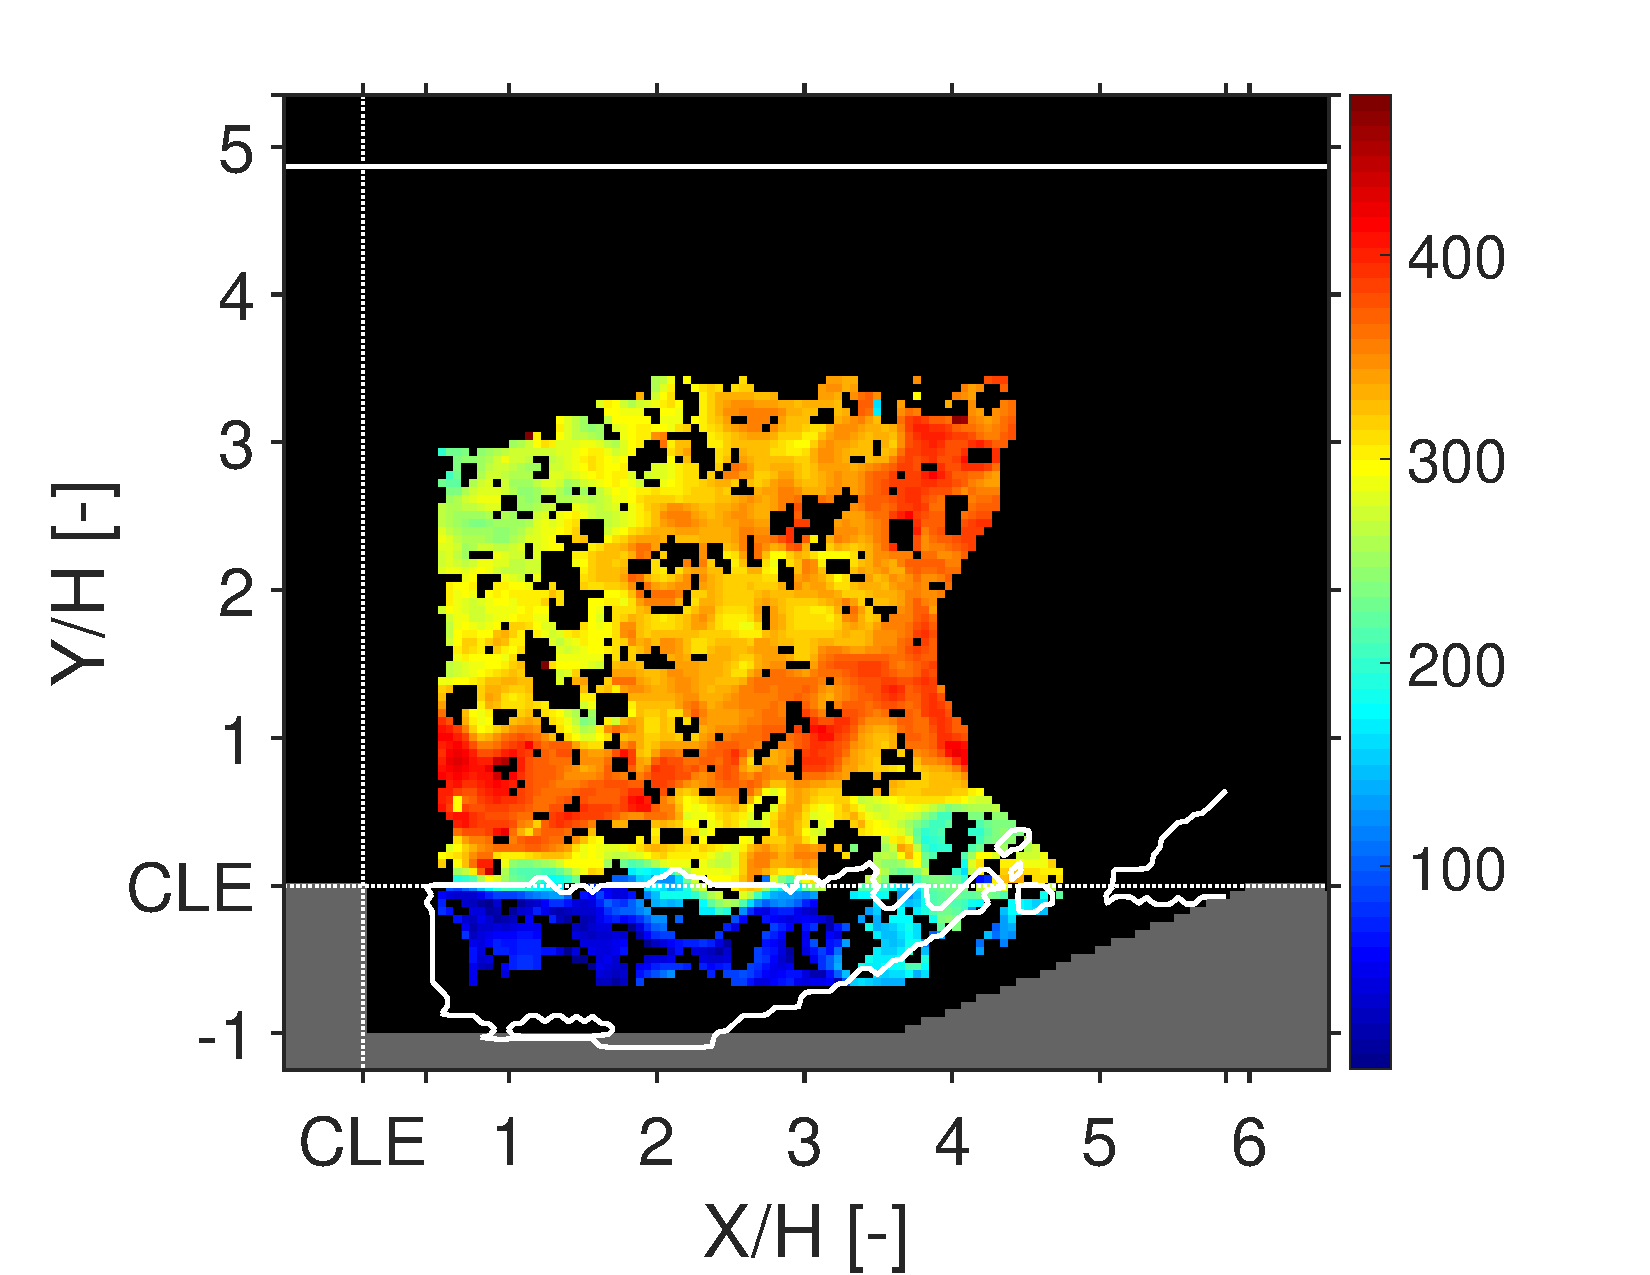
\includegraphics[width=3in,trim=0.35in 0 0.65in 0, clip]{figures/B1/combustion_instability/3/absolute_vel/B1_Frame339.pdf}\rotatebox{90}{\hspace{1.3in}\footnotesize$\mathrm{[m/s]}$}}
                \newline
 \subcaptionbox{State 3'\label{fig:B1_Frame5}}
                {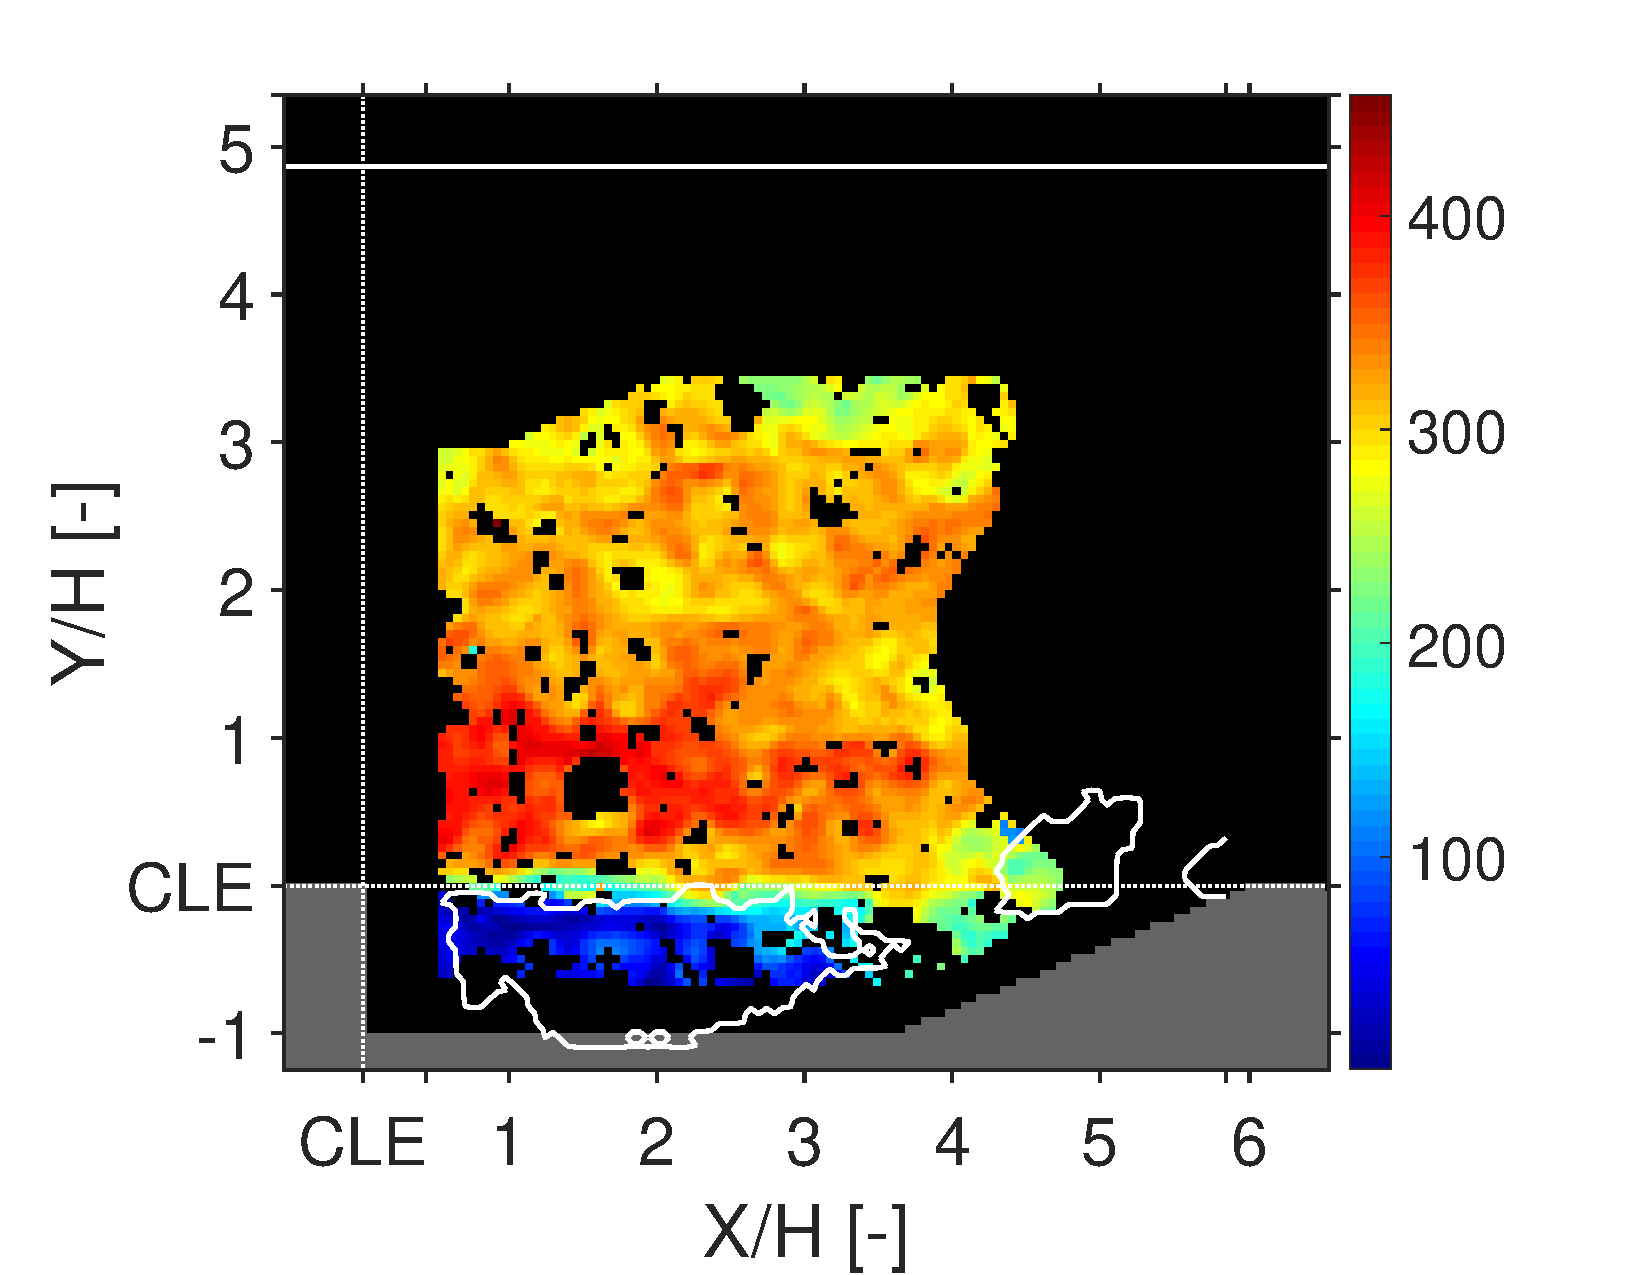
\includegraphics[width=3in,trim=0.35in 0 0.65in 0, clip]{figures/B1/combustion_instability/3/absolute_vel/B1_Frame306.pdf}\rotatebox{90}{\hspace{1.3in}\footnotesize$\mathrm{[m/s]}$}}
                \hspace{0.4cm}
        \subcaptionbox{State 2 with duct velocities below average\label{fig:B1_Frame6}}
                {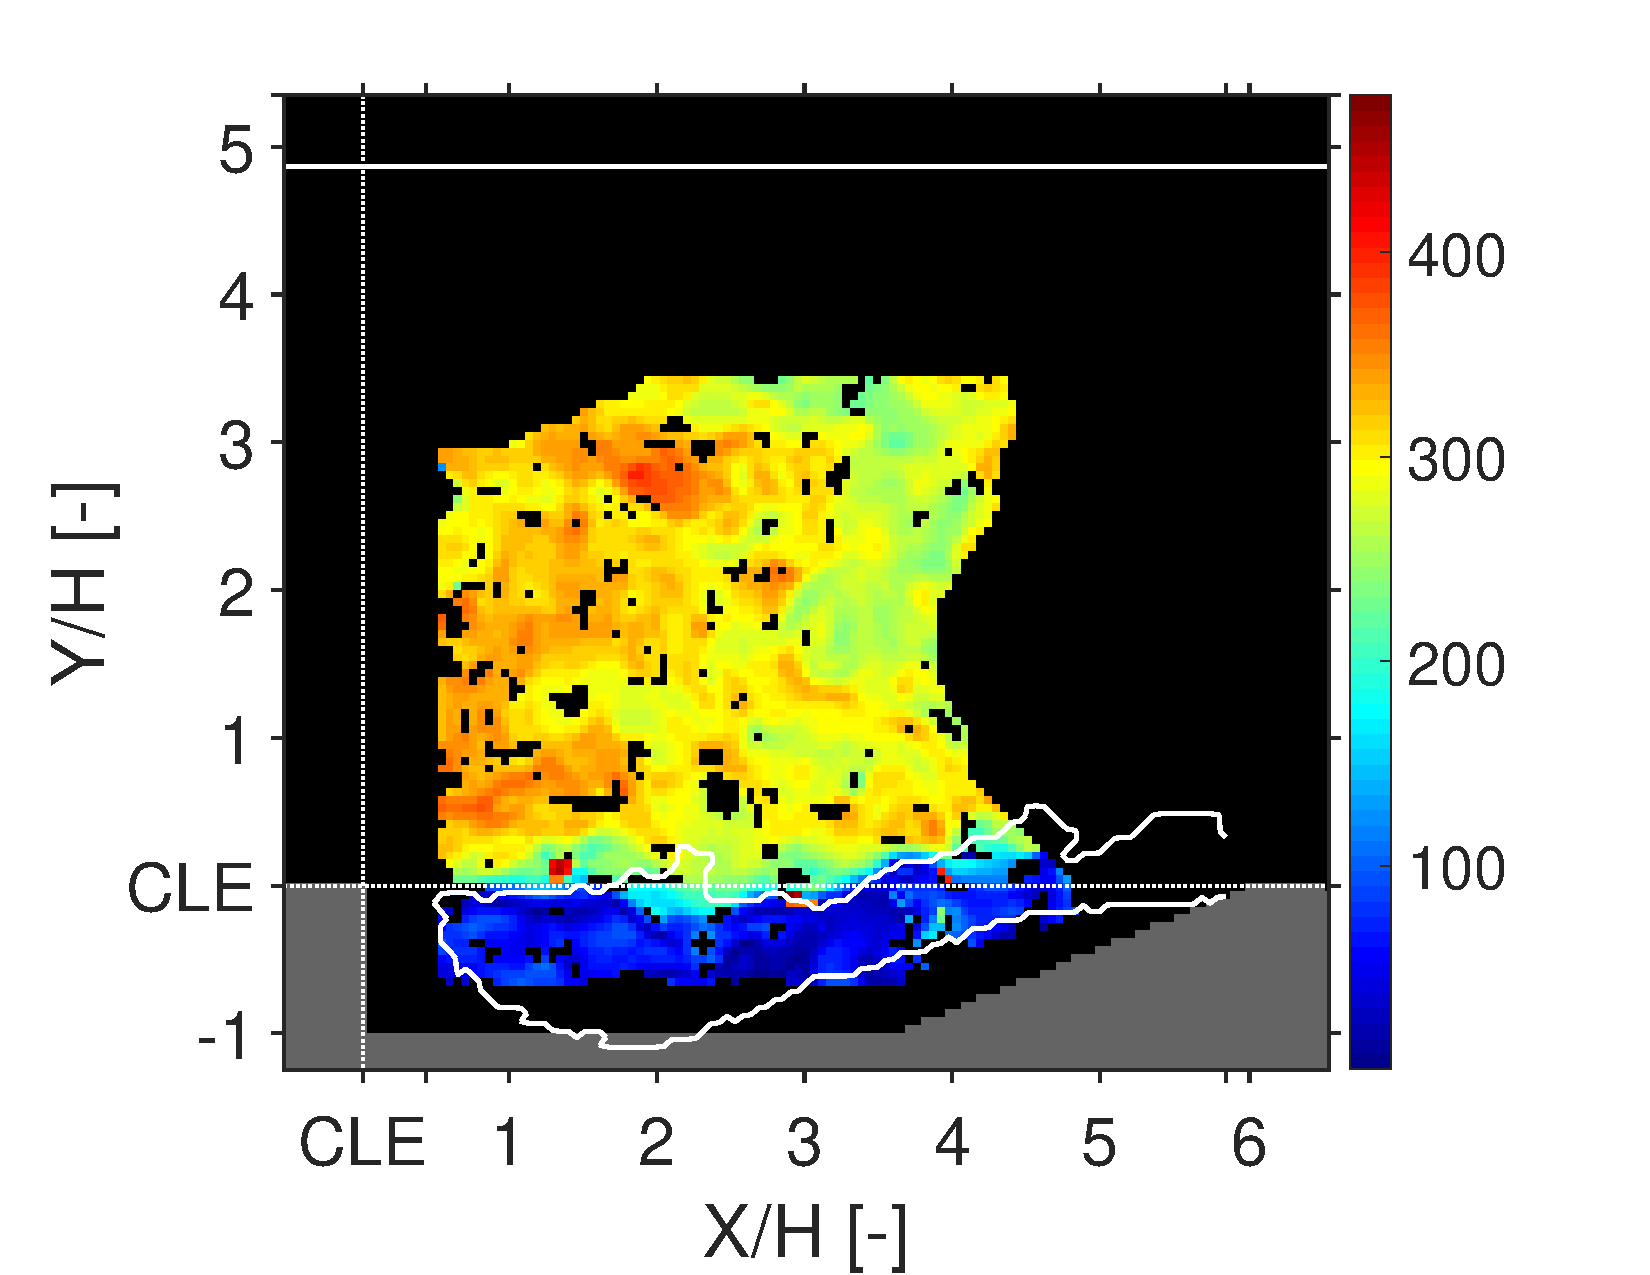
\includegraphics[width=3in,trim=0.35in 0 0.65in 0, clip]{figures/B1/combustion_instability/2/absolute_vel/B1_Frame301.pdf}\rotatebox{90}{\hspace{1.3in}\footnotesize$\mathrm{[m/s]}$}}
\caption{Velocity magnitude, select instantaneous PIV-PLIF frames.}\label{fig:ch3_inst_B1}
\end{figure}

% \begin{figure}
% \centering
% \subcaptionbox{State 1\label{fig:B1_Frame1}}
%         {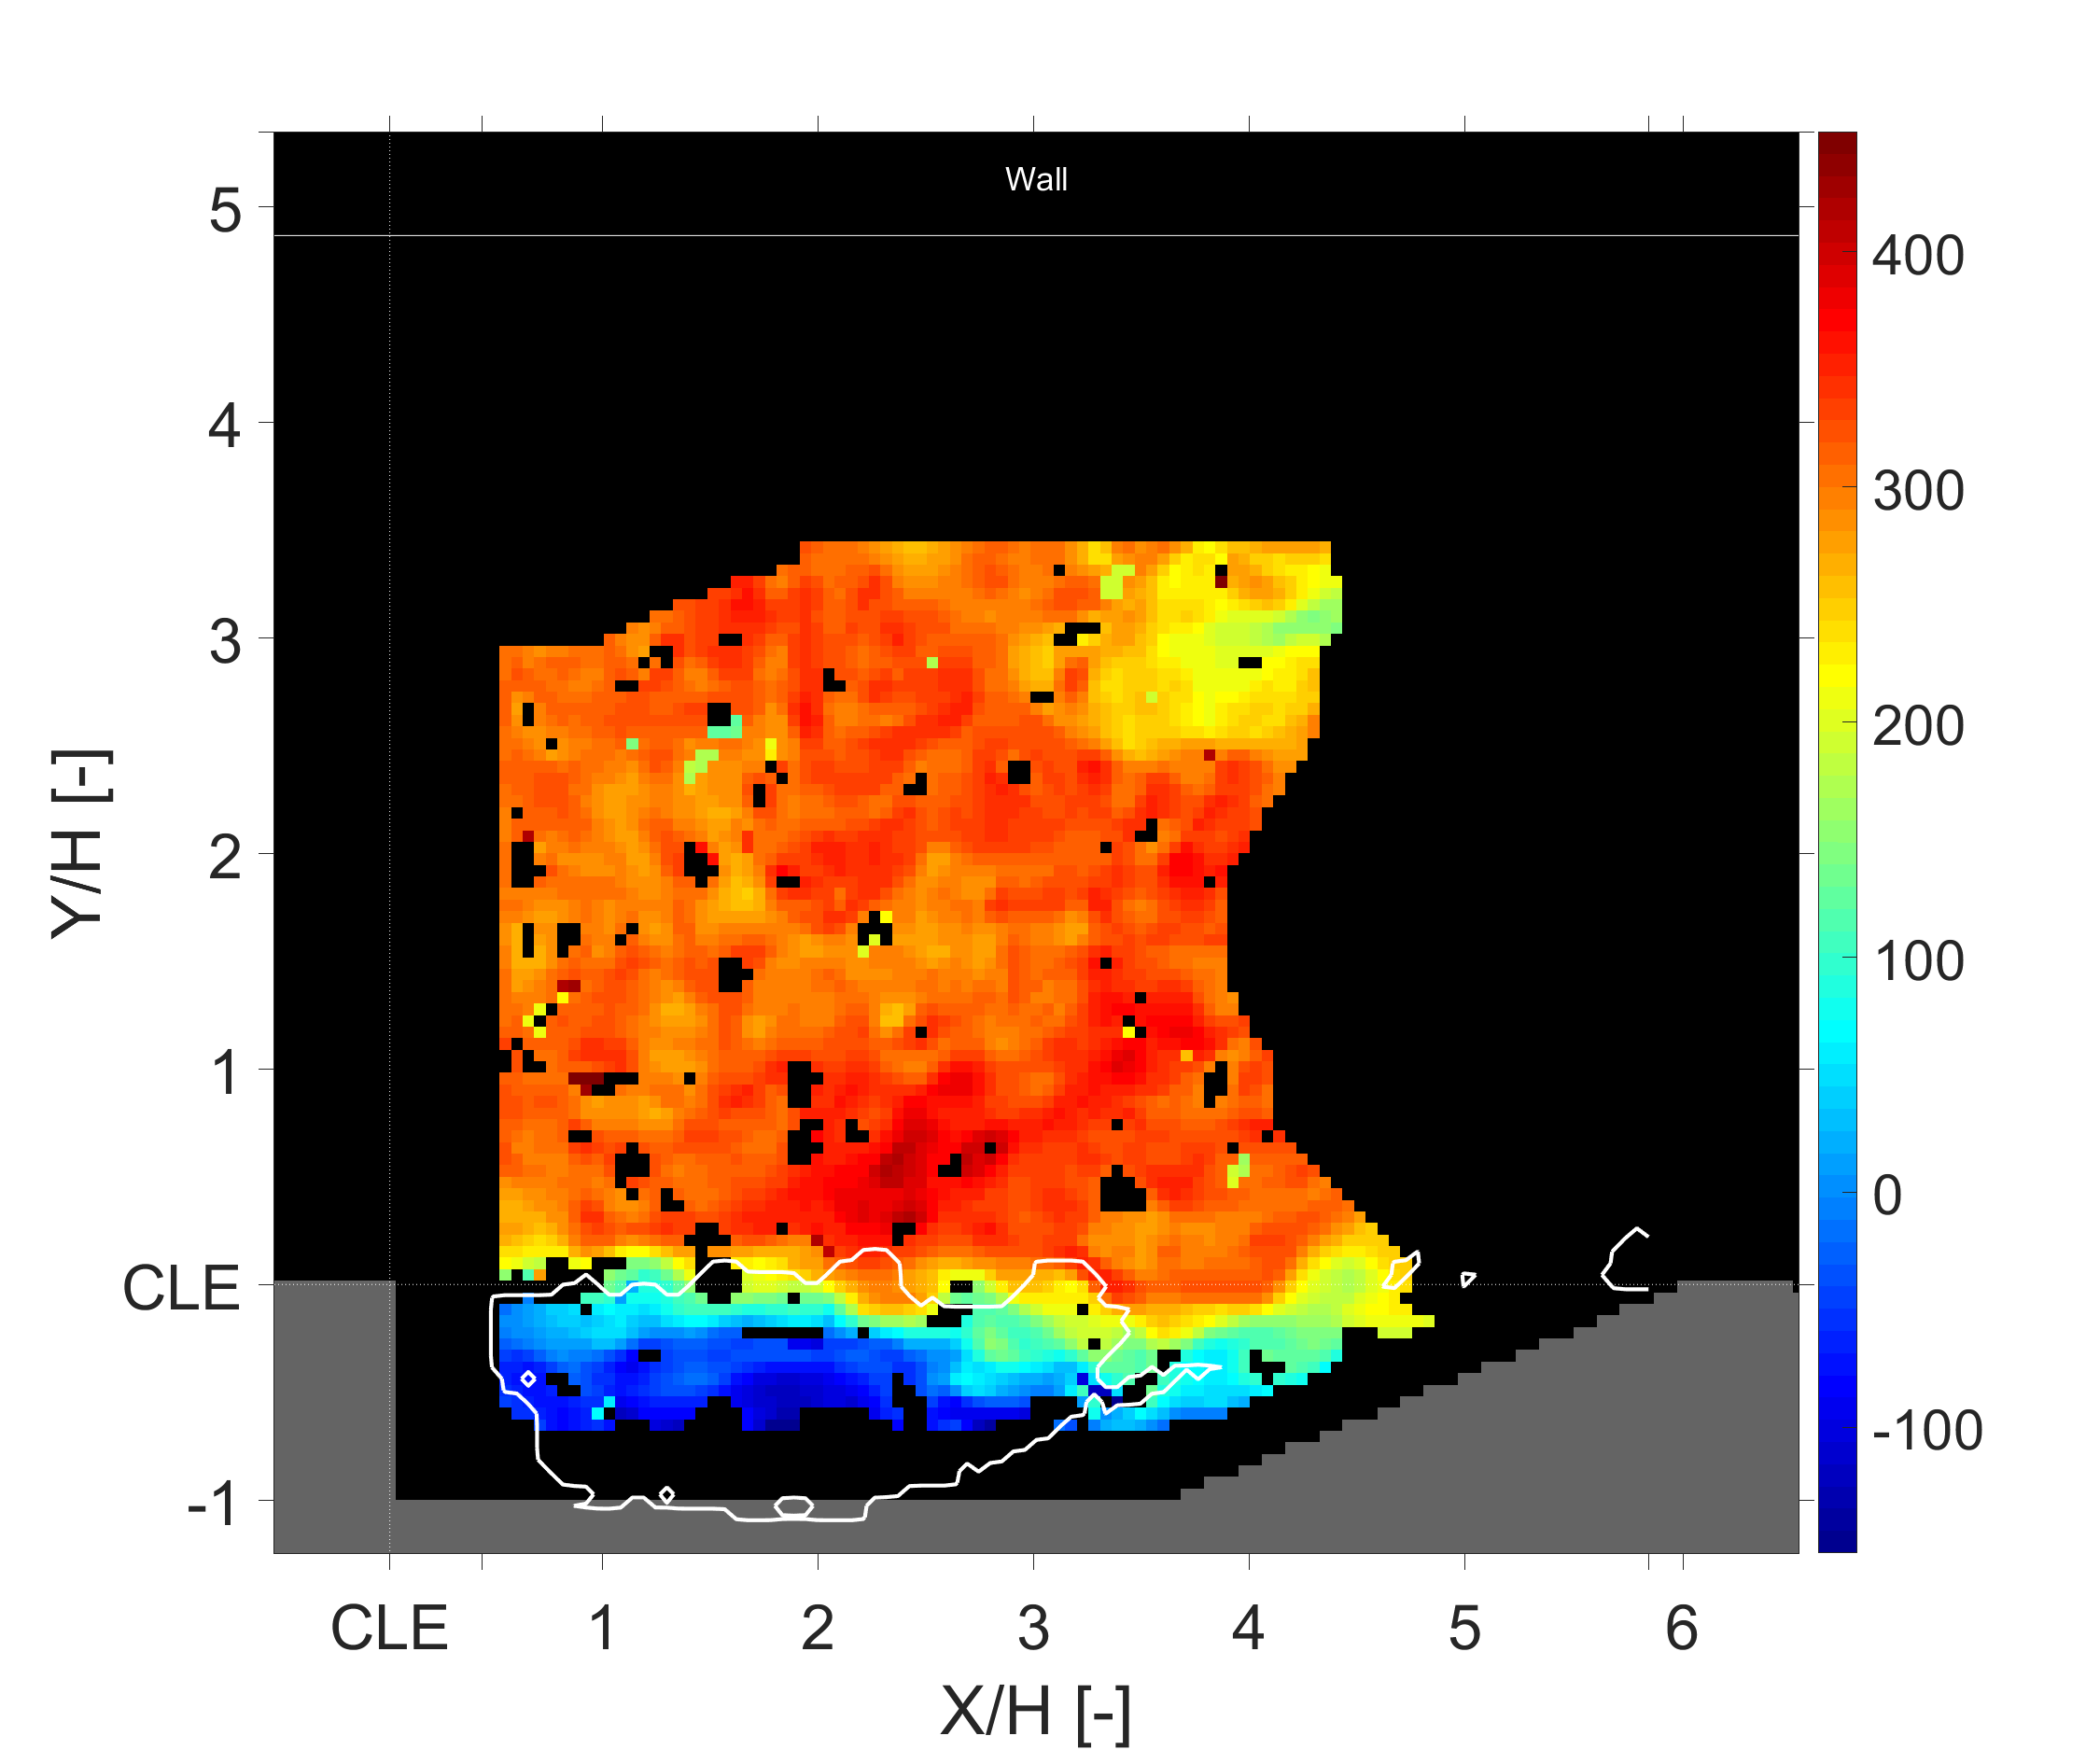
\includegraphics[height=2.5in, trim=0cm 0cm 0cm 0cm, clip]{figures/B1/combustion_instability/x/B1_Frame331_x}\hspace{0.5cm}} %pdfcrop
% \subcaptionbox{State 2\label{fig:B1_Frame2}}
%         {\hspace{0.5cm}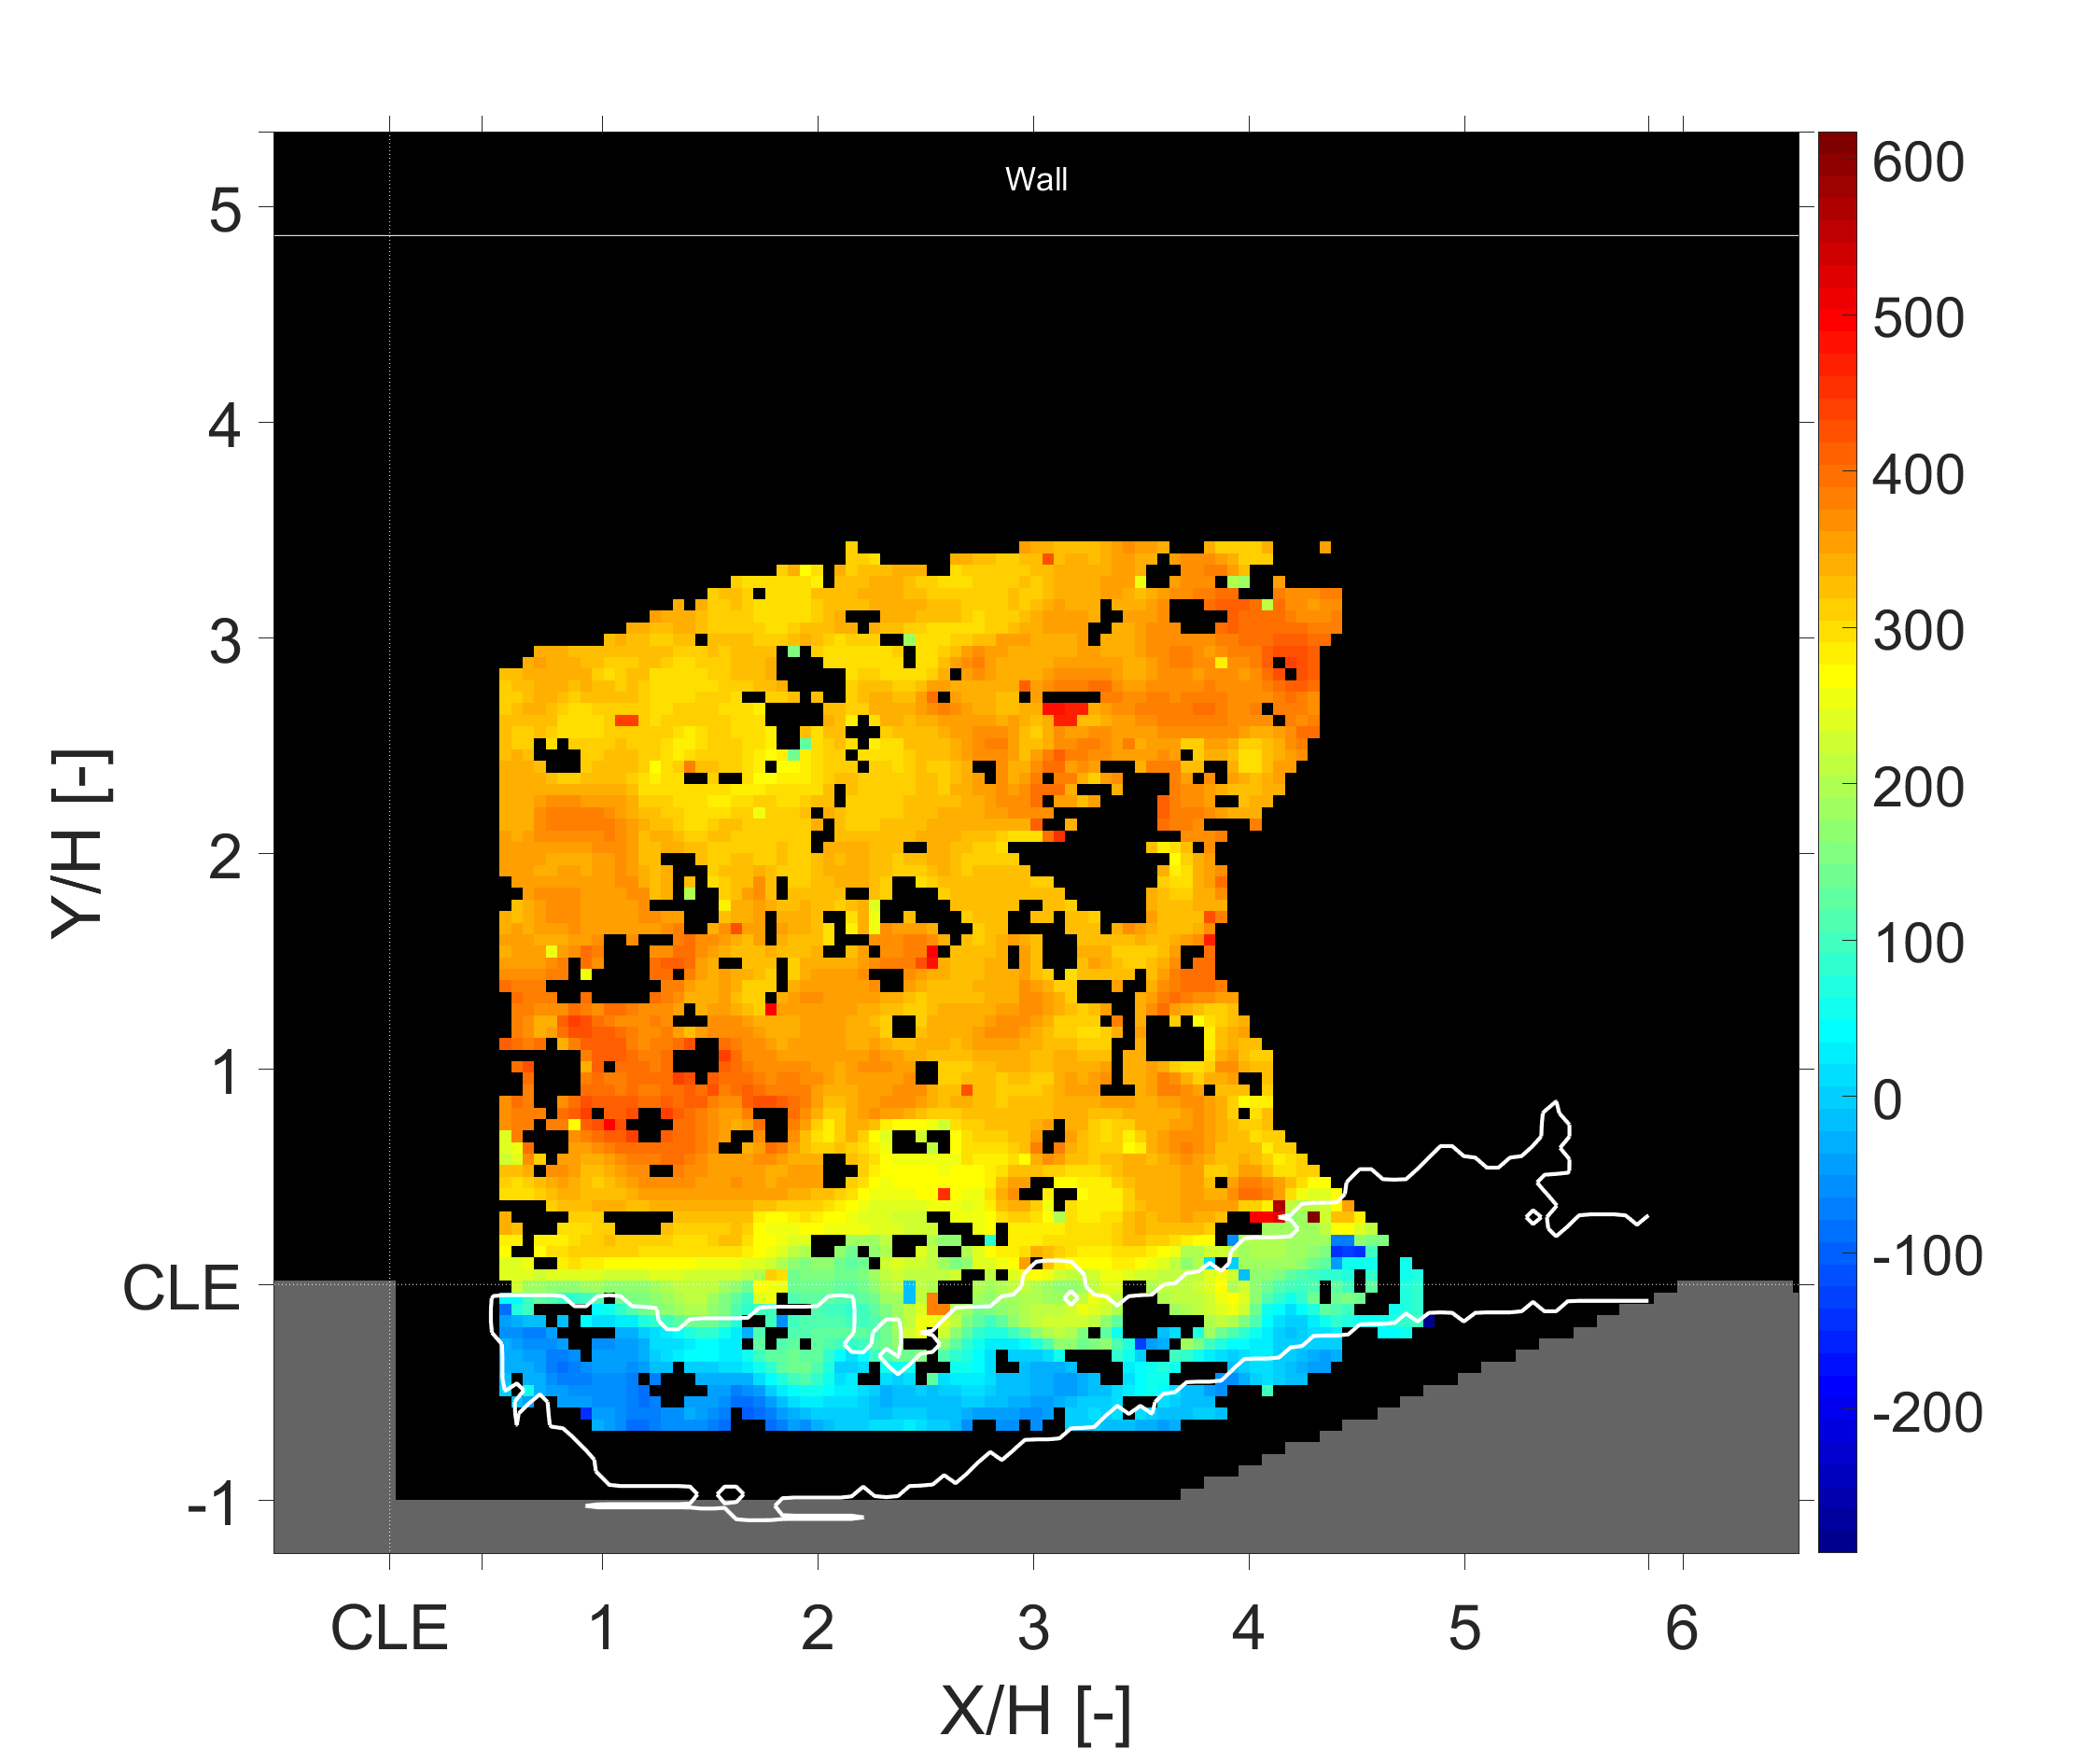
\includegraphics[height=2.5in, trim=0cm 0cm 0cm 0cm, clip]{figures/B1/combustion_instability/x/B1_Frame329_x}}
% \subcaptionbox{State 3\label{fig:B1_Frame3}}
%         {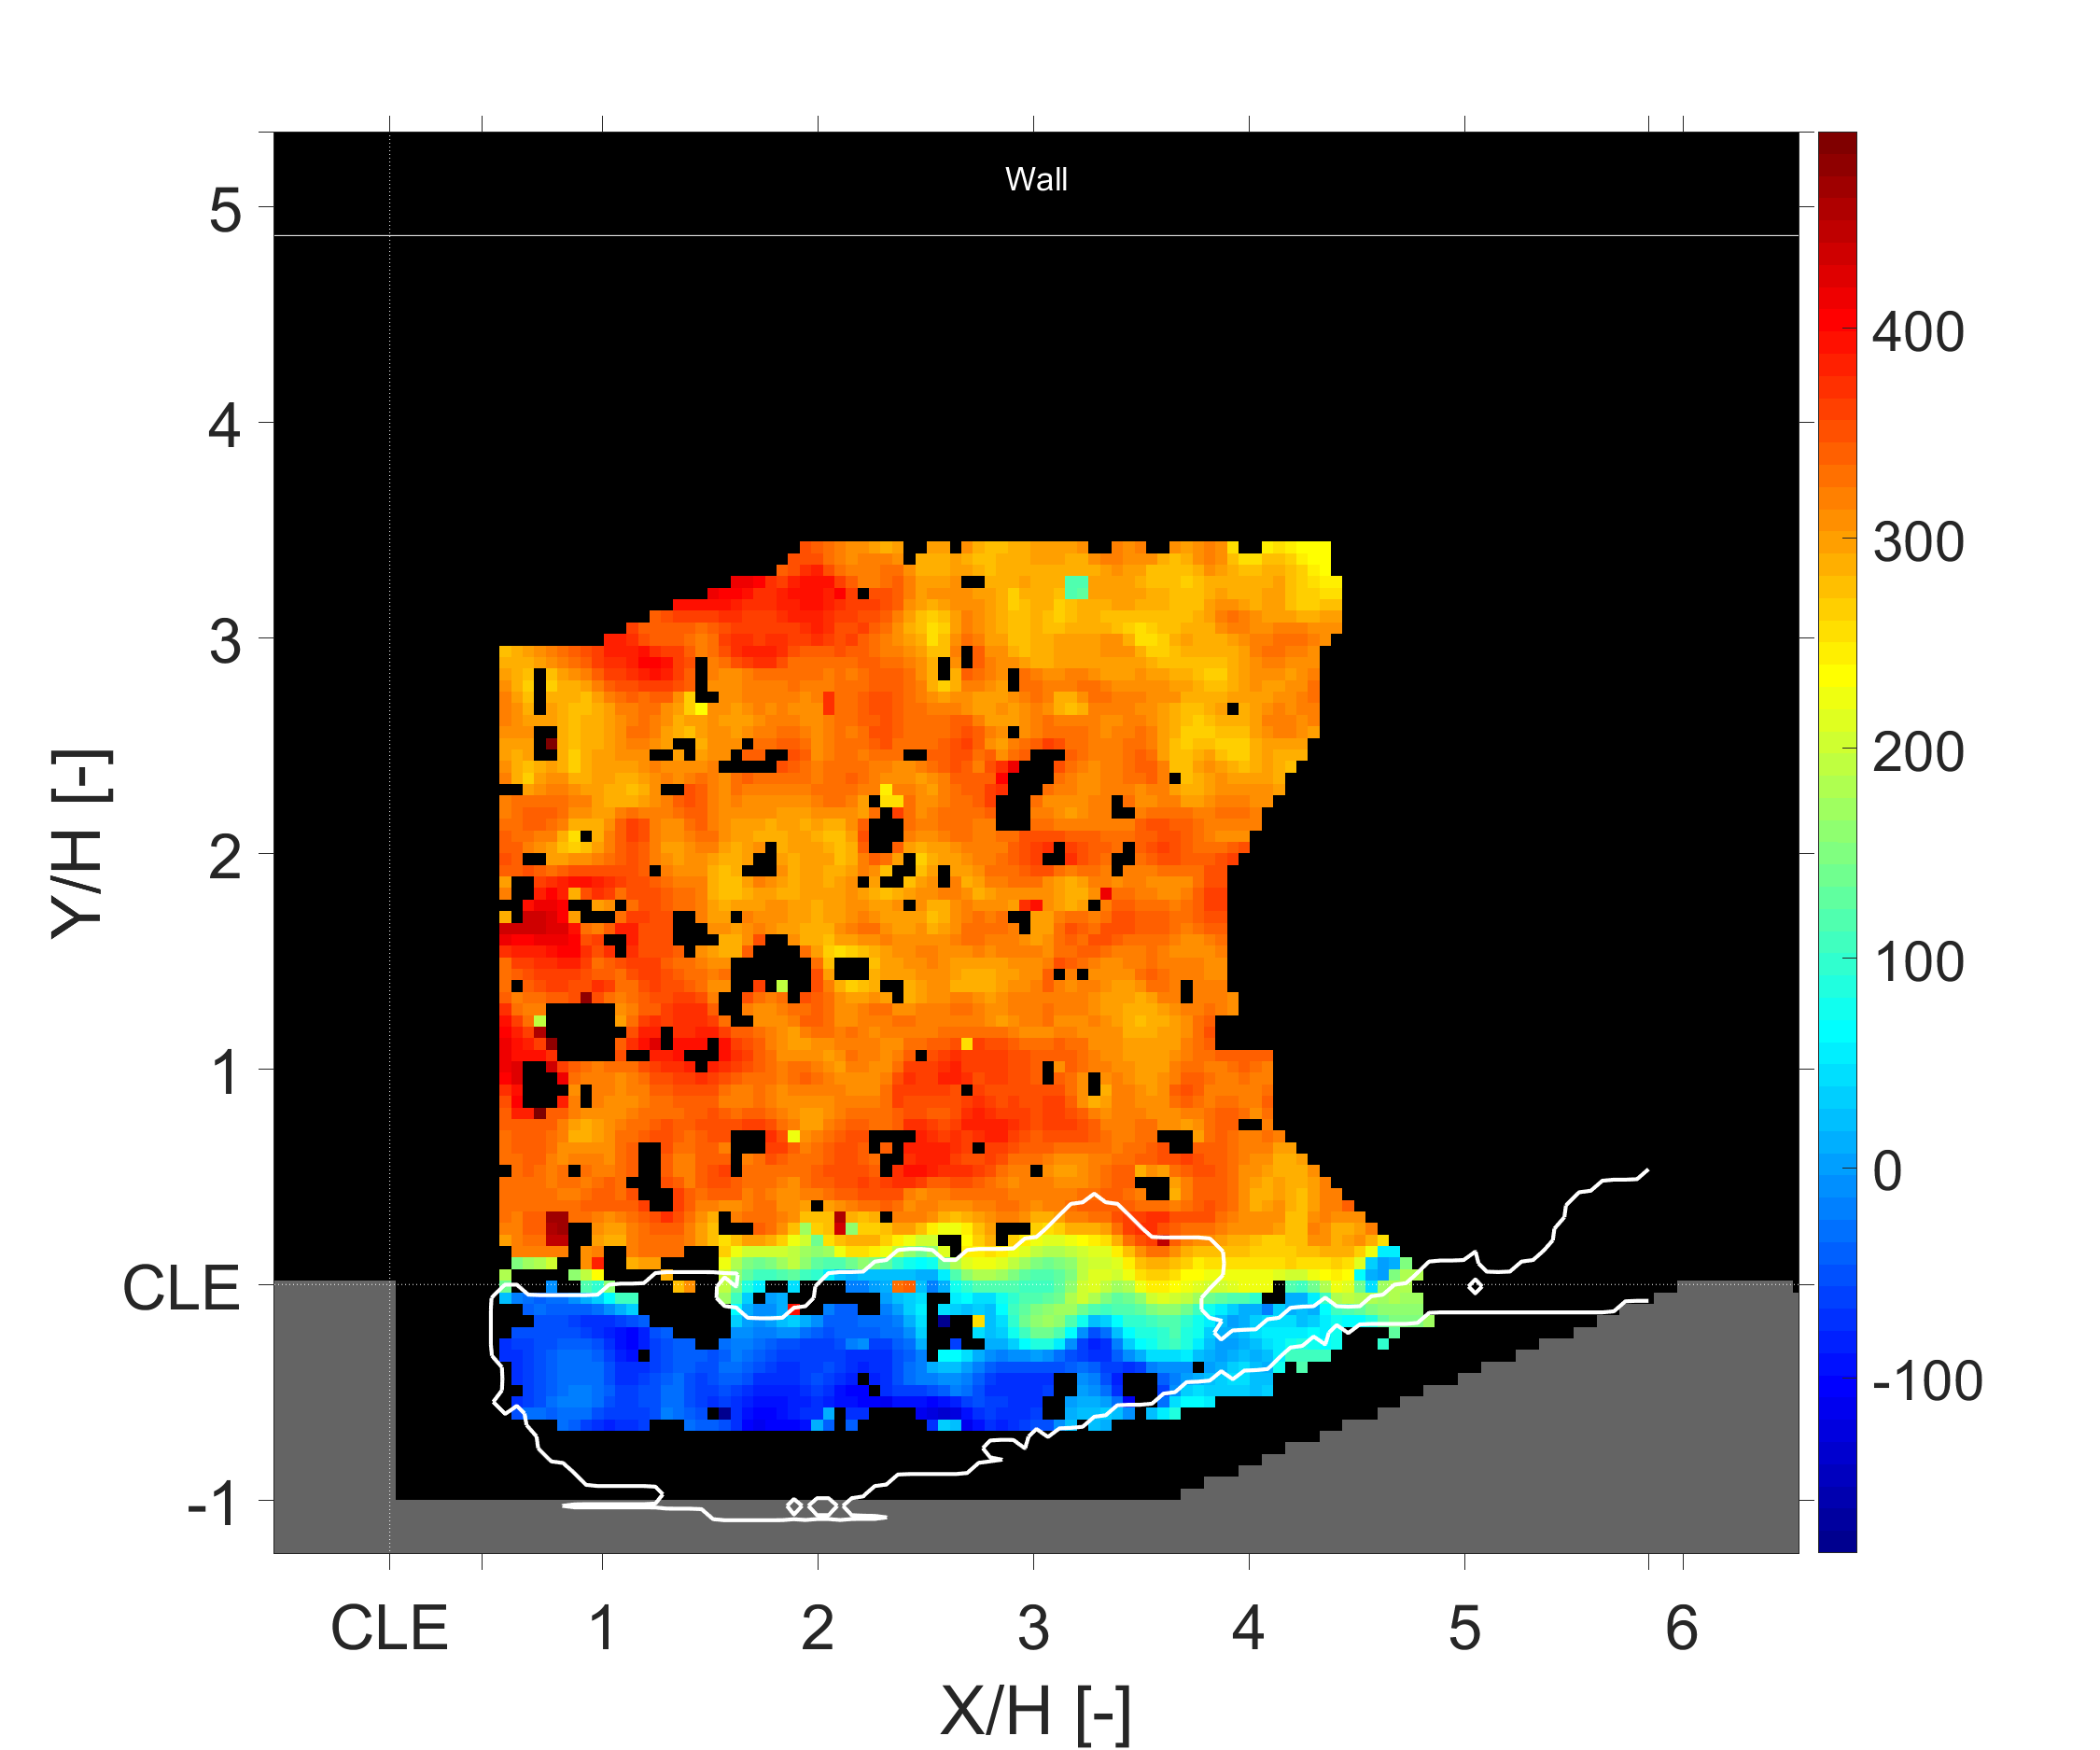
\includegraphics[height=2.5in, trim=0cm 0cm 0cm 0cm, clip]{figures/B1/combustion_instability/x/B1_Frame342_x}\hspace{0.5cm}}
% \subcaptionbox{State 4\label{fig:B1_Frame4}}
%         {\hspace{0.5cm}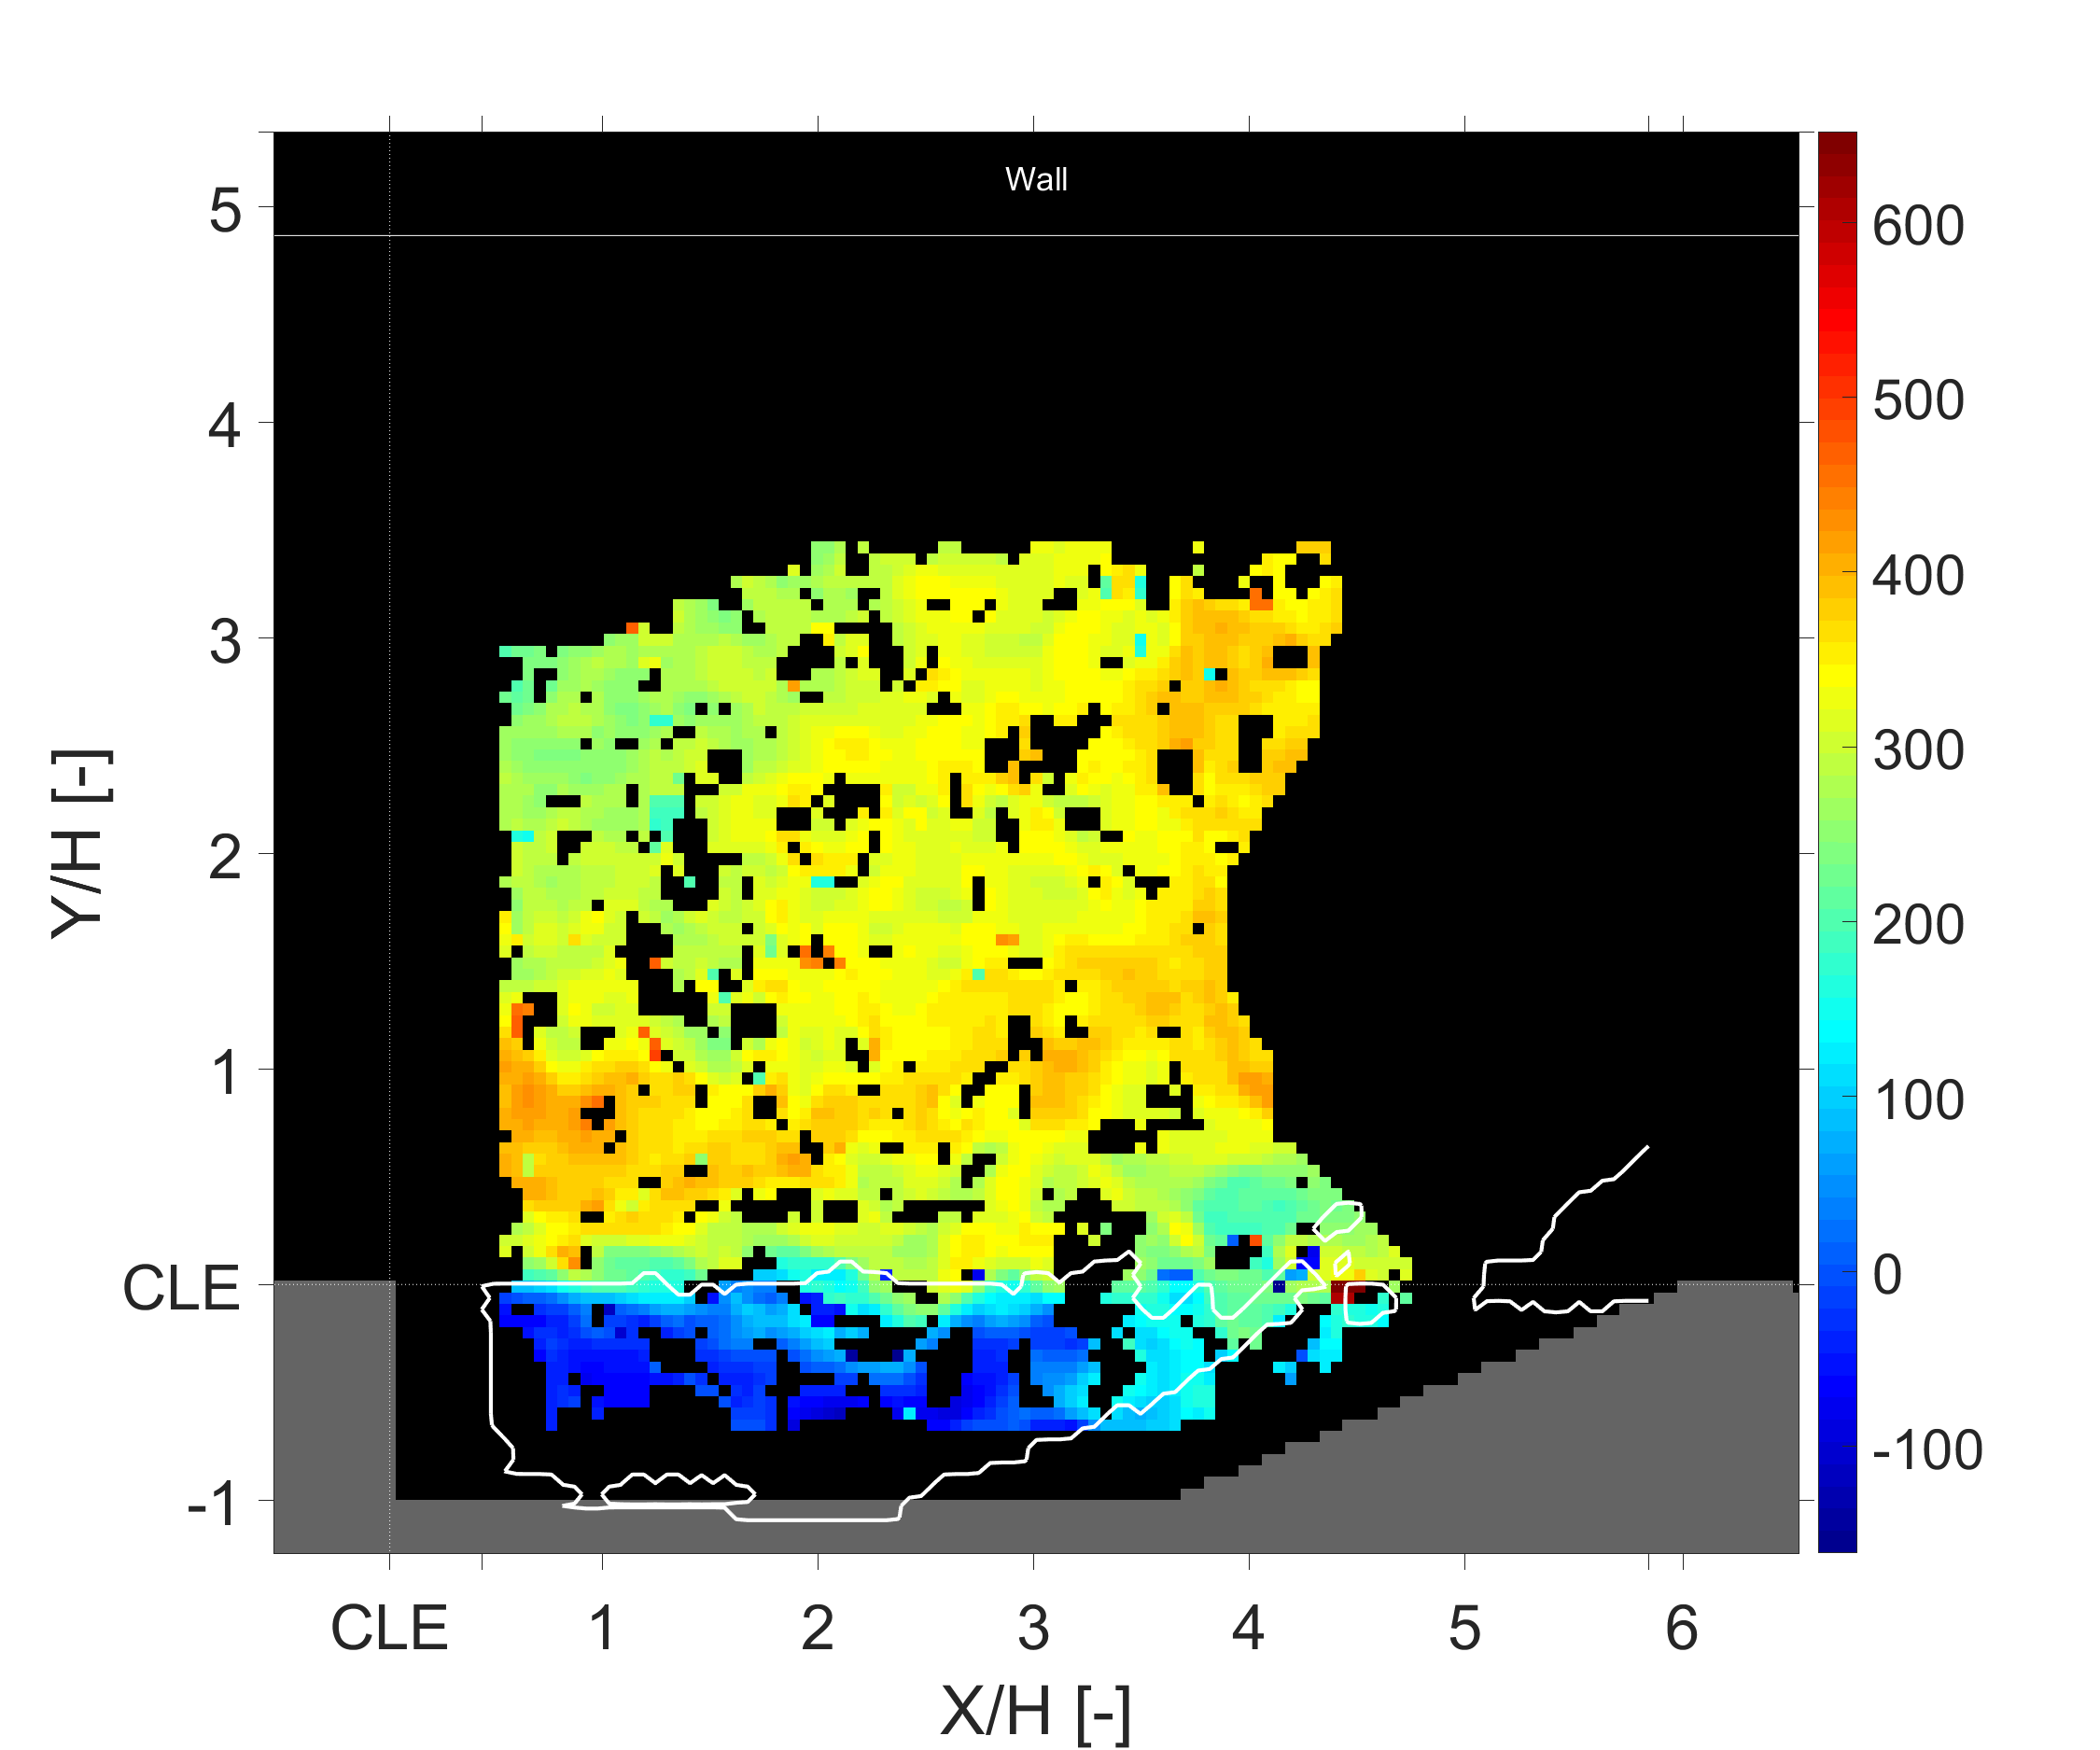
\includegraphics[height=2.5in, trim=0cm 0cm 0cm 0cm, clip]{figures/B1/combustion_instability/x/B1_Frame339_x}}
% \subcaptionbox{State 5\label{fig:B1_Frame5}}
%         {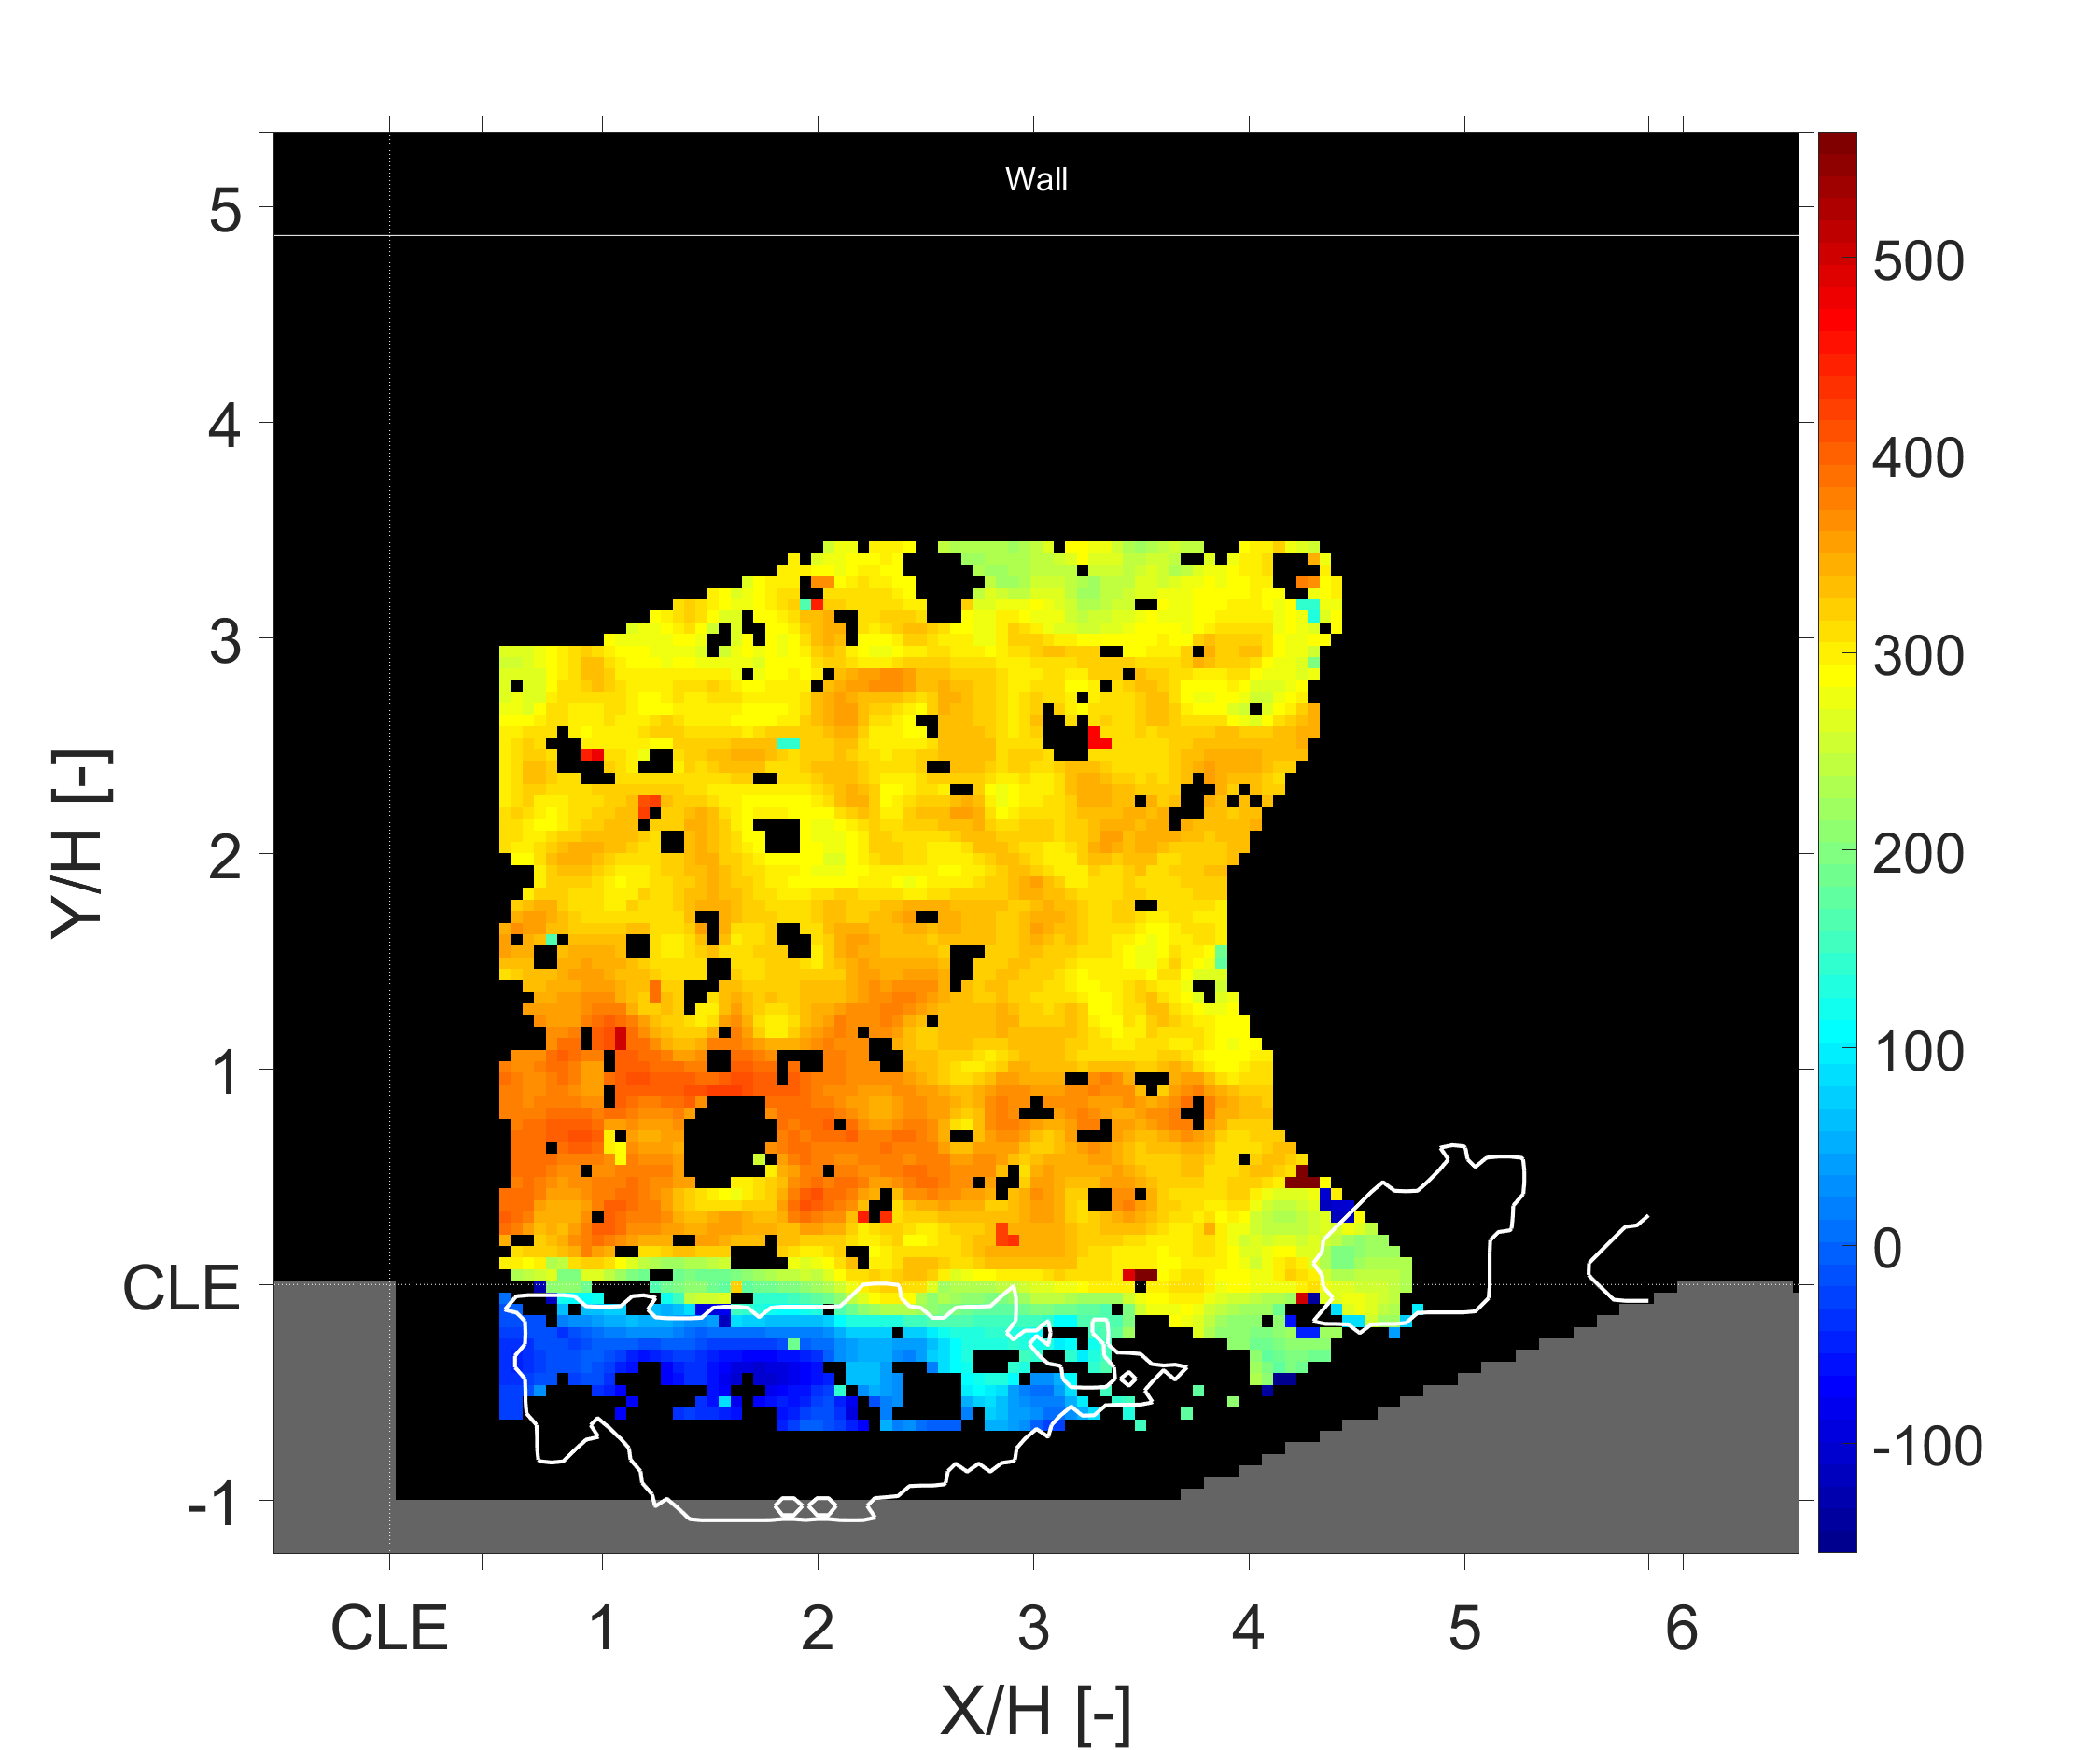
\includegraphics[height=2.5in, trim=0cm 0cm 0cm 0cm, clip]{figures/B1/combustion_instability/x/B1_Frame306_x.png}\hspace{0.5cm}}
%         \subcaptionbox{State 2 with duct velocities below average\label{fig:B1_Frame6}}
%         {\hspace{0.5cm}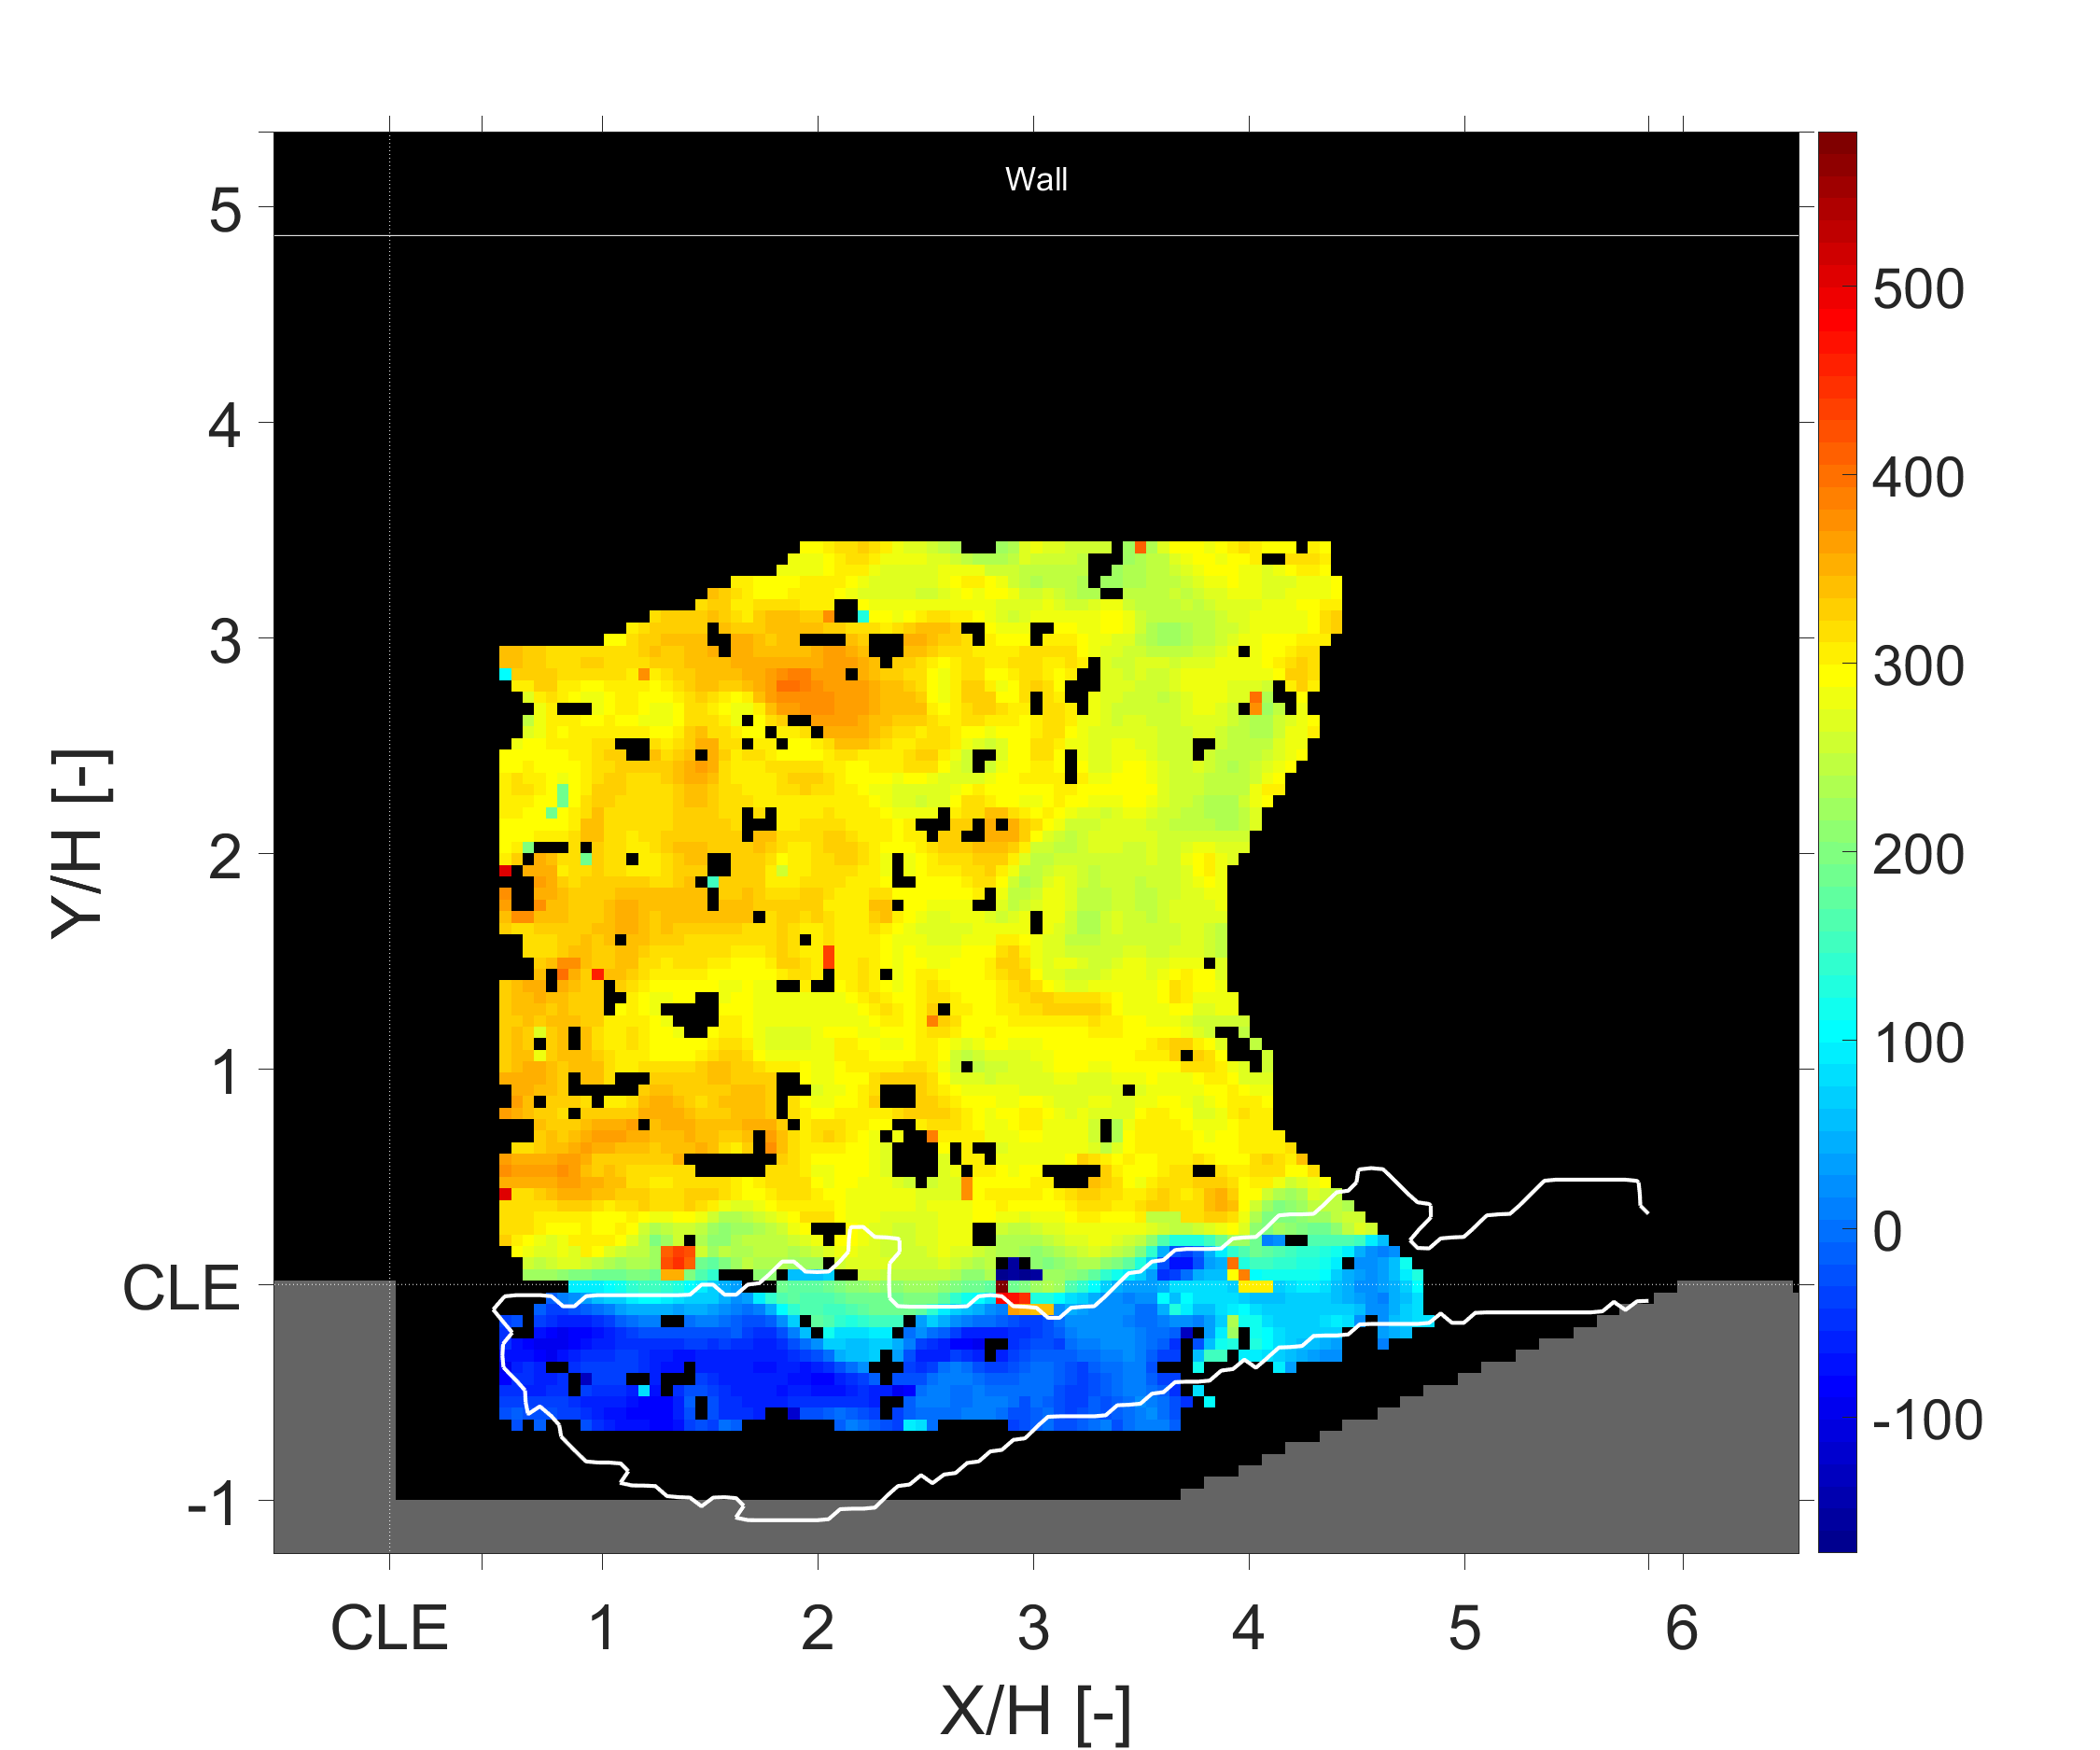
\includegraphics[height=2.5in, trim=0cm 0cm 0cm 0cm, clip]{figures/B1/combustion_instability/x/B1_Frame301_x}}
% \caption{$U_x$, select instantaneous PIV-PLIF frames.}\label{fig:ch3_inst_B1}
% \end{figure}

% \begin{figure}
% \centering
% \subcaptionbox{State 1\label{fig:B1_Frame1y}}
%         {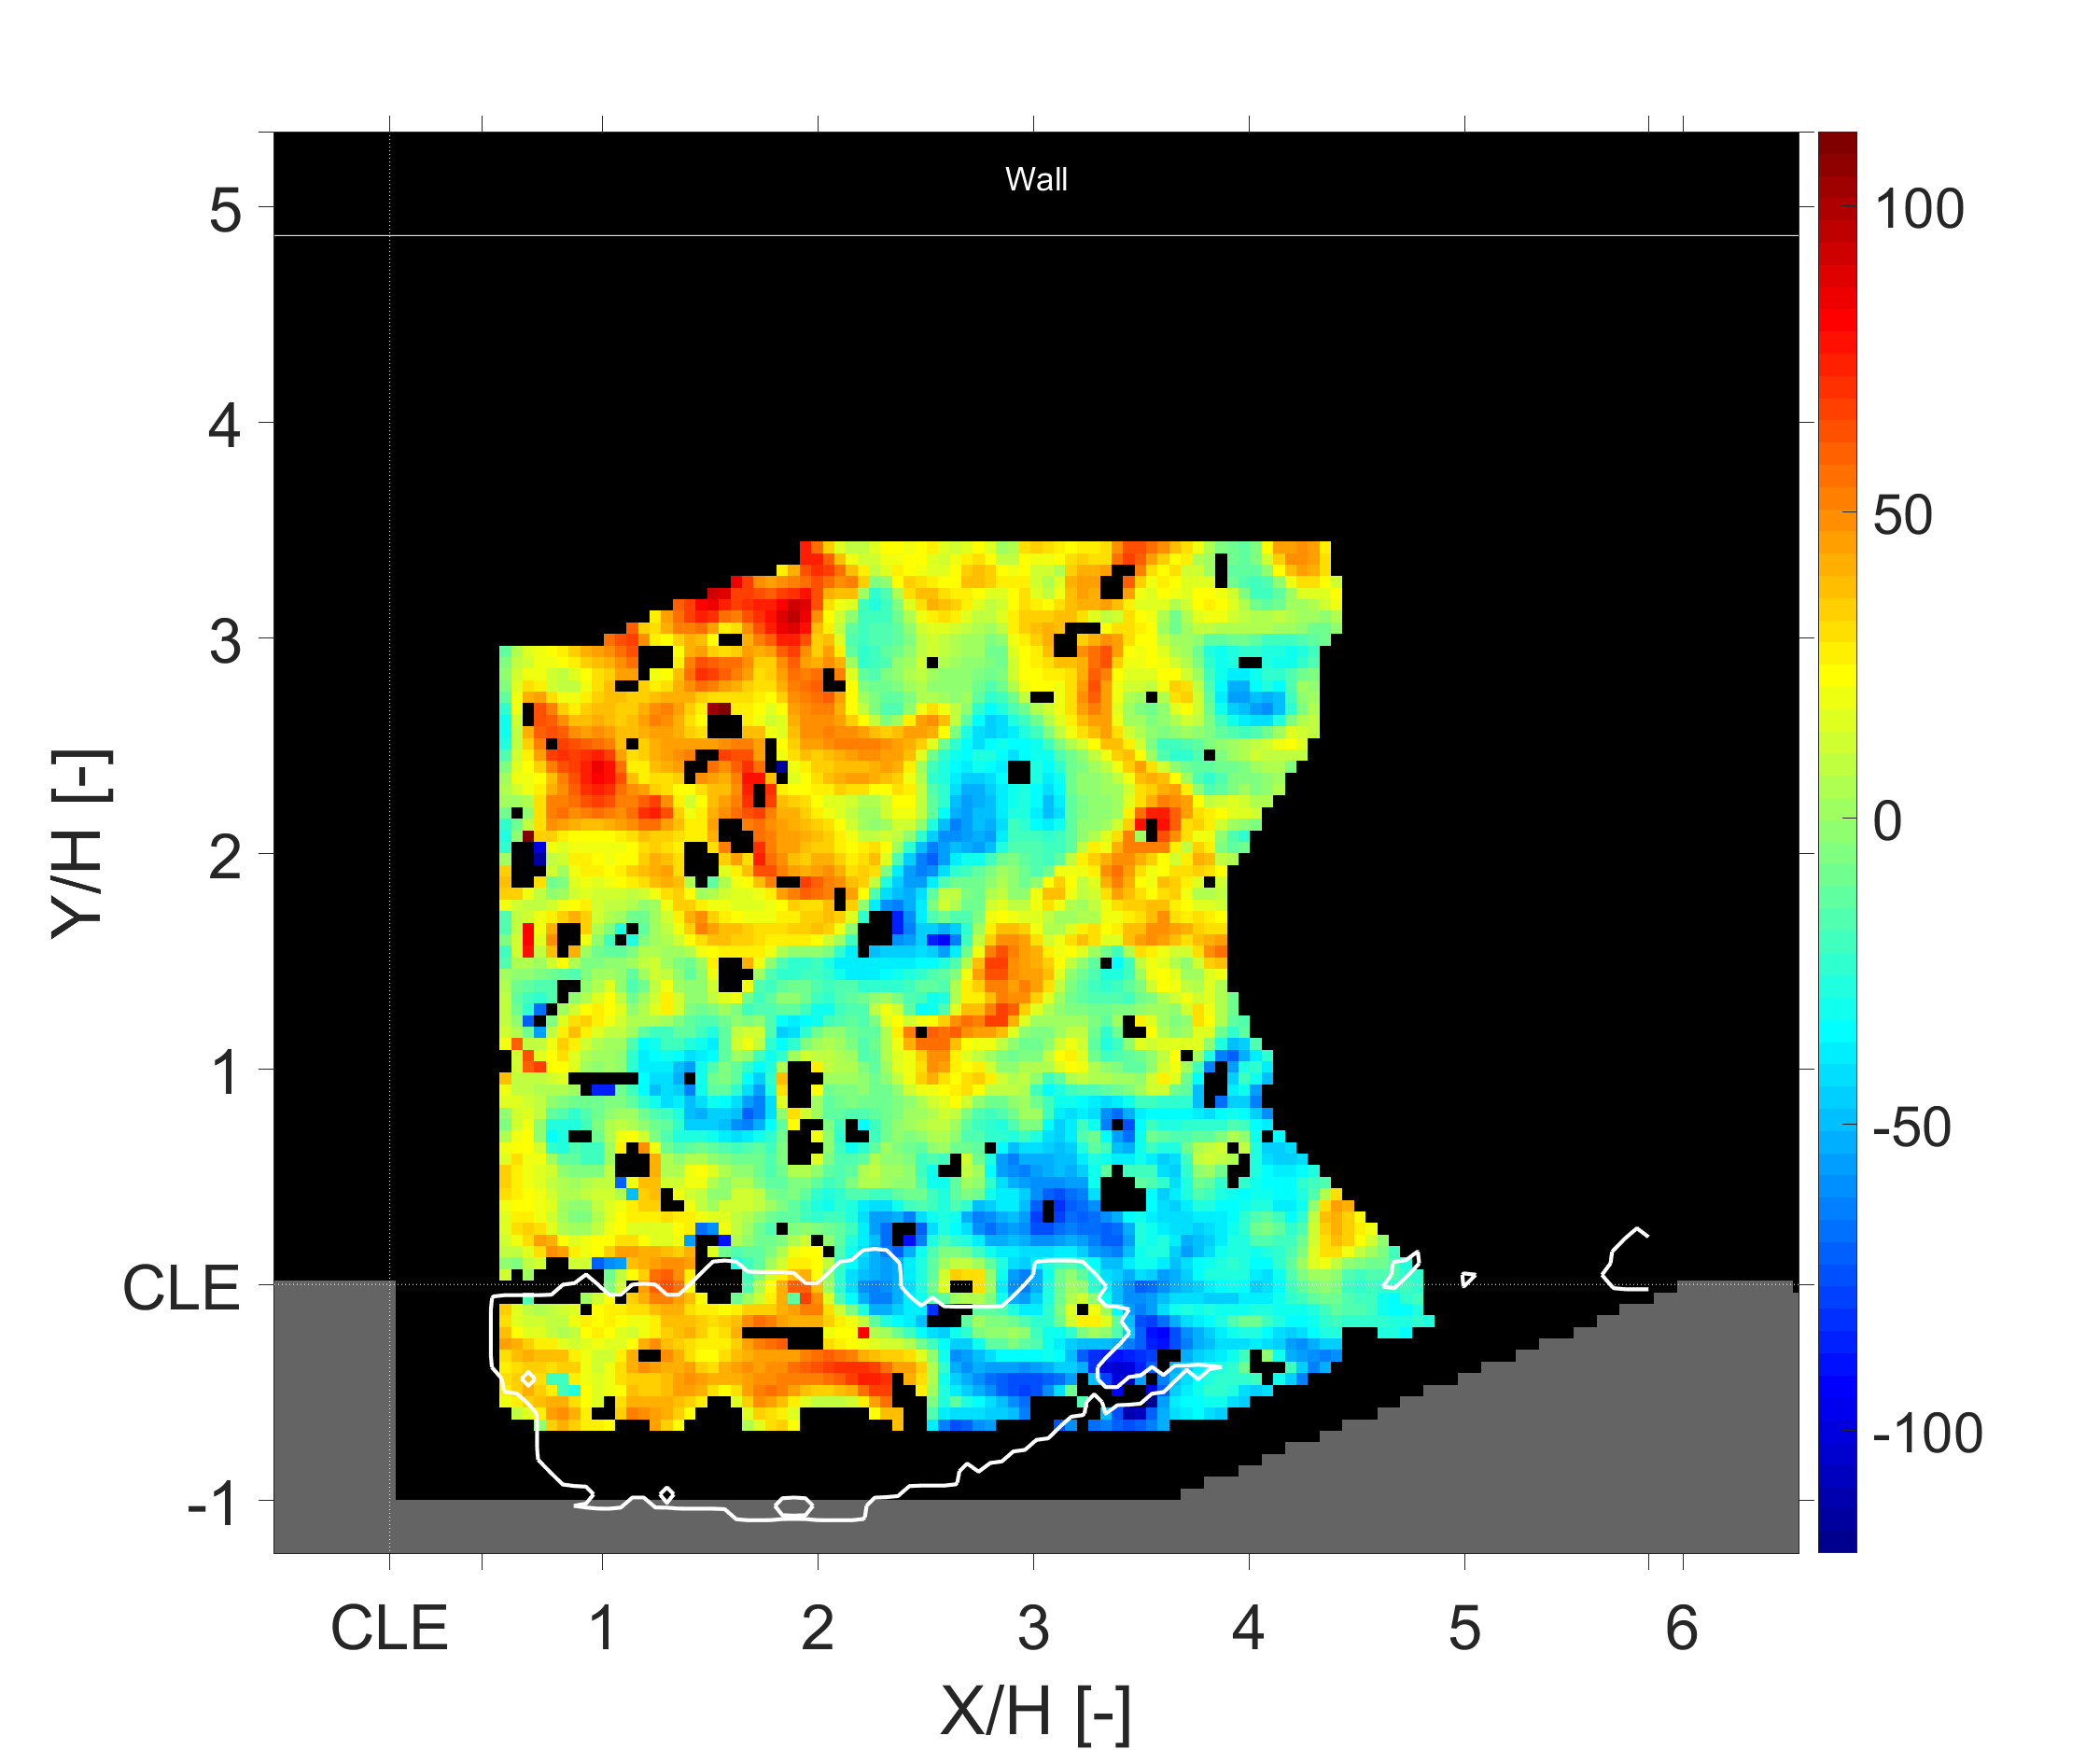
\includegraphics[height=2.5in, trim=0cm 0cm 0cm 0cm, clip]{figures/B1/combustion_instability/y/B1_Frame331_y}\hspace{0.5cm}} %pdfcrop
% \subcaptionbox{State 2\label{fig:B1_Frame2y}}
%         {\hspace{0.5cm}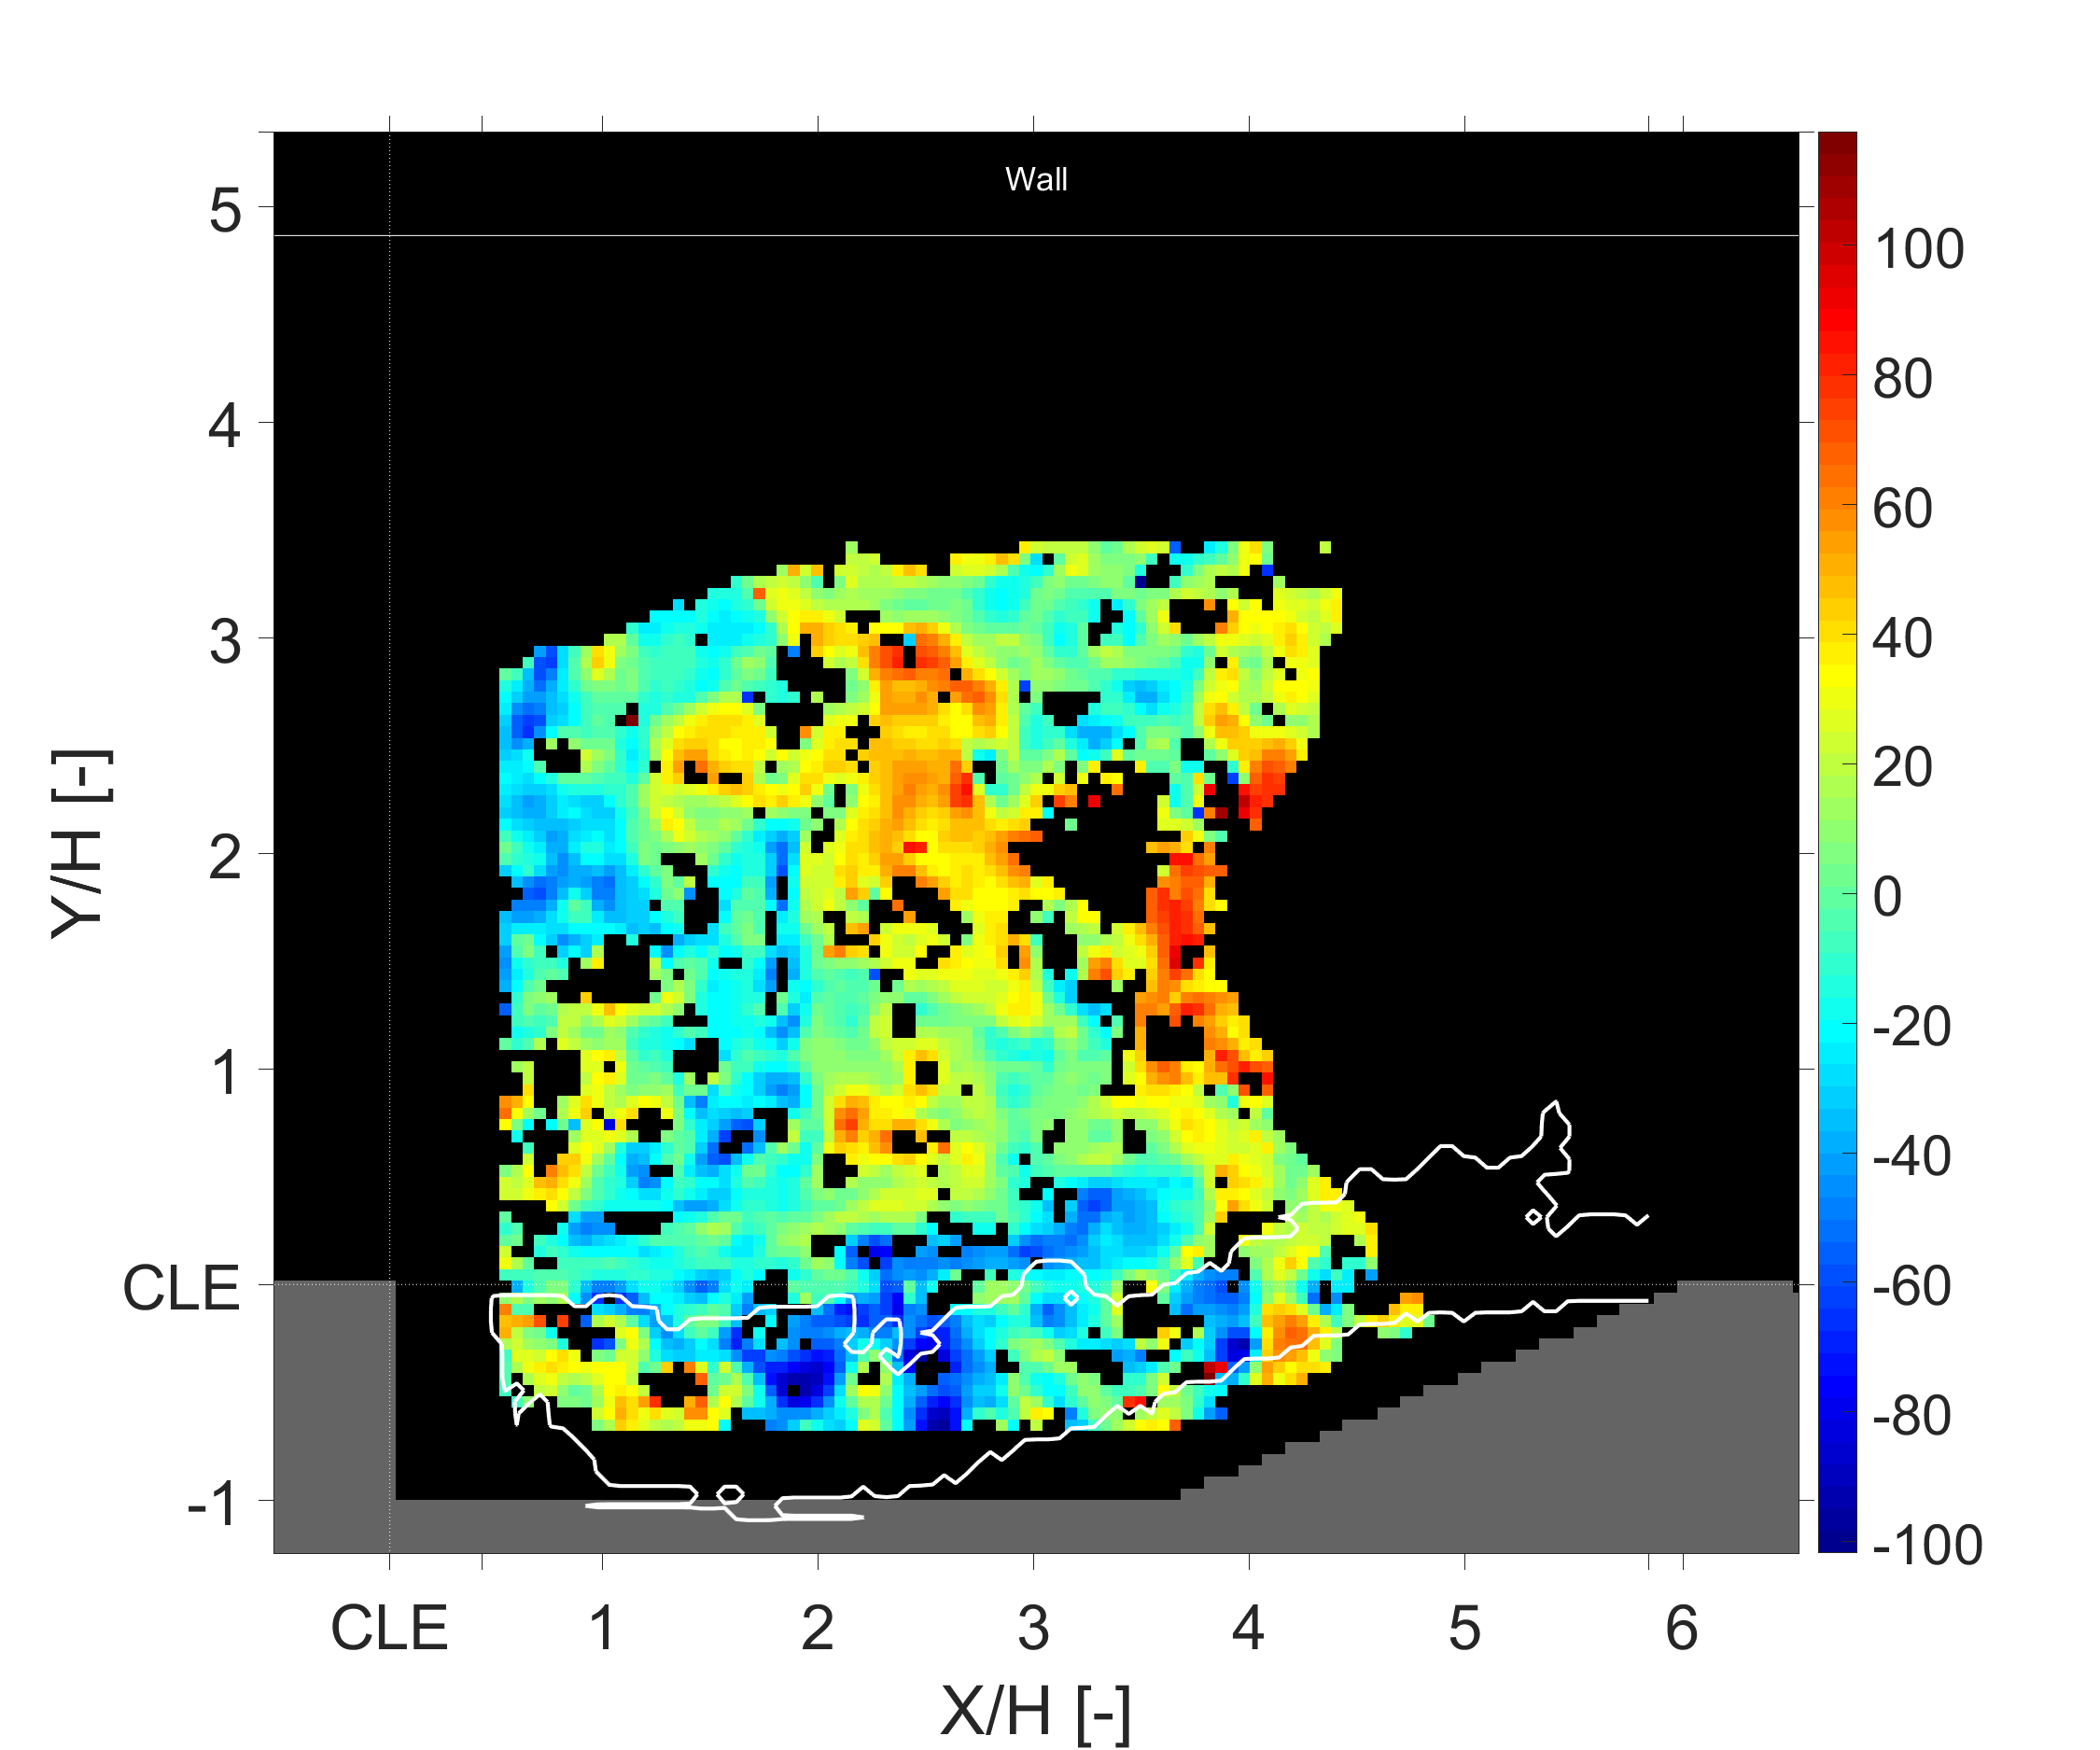
\includegraphics[height=2.5in, trim=0cm 0cm 0cm 0cm, clip]{figures/B1/combustion_instability/y/B1_Frame329_y}}
% \subcaptionbox{State 3\label{fig:B1_Frame3y}}
%         {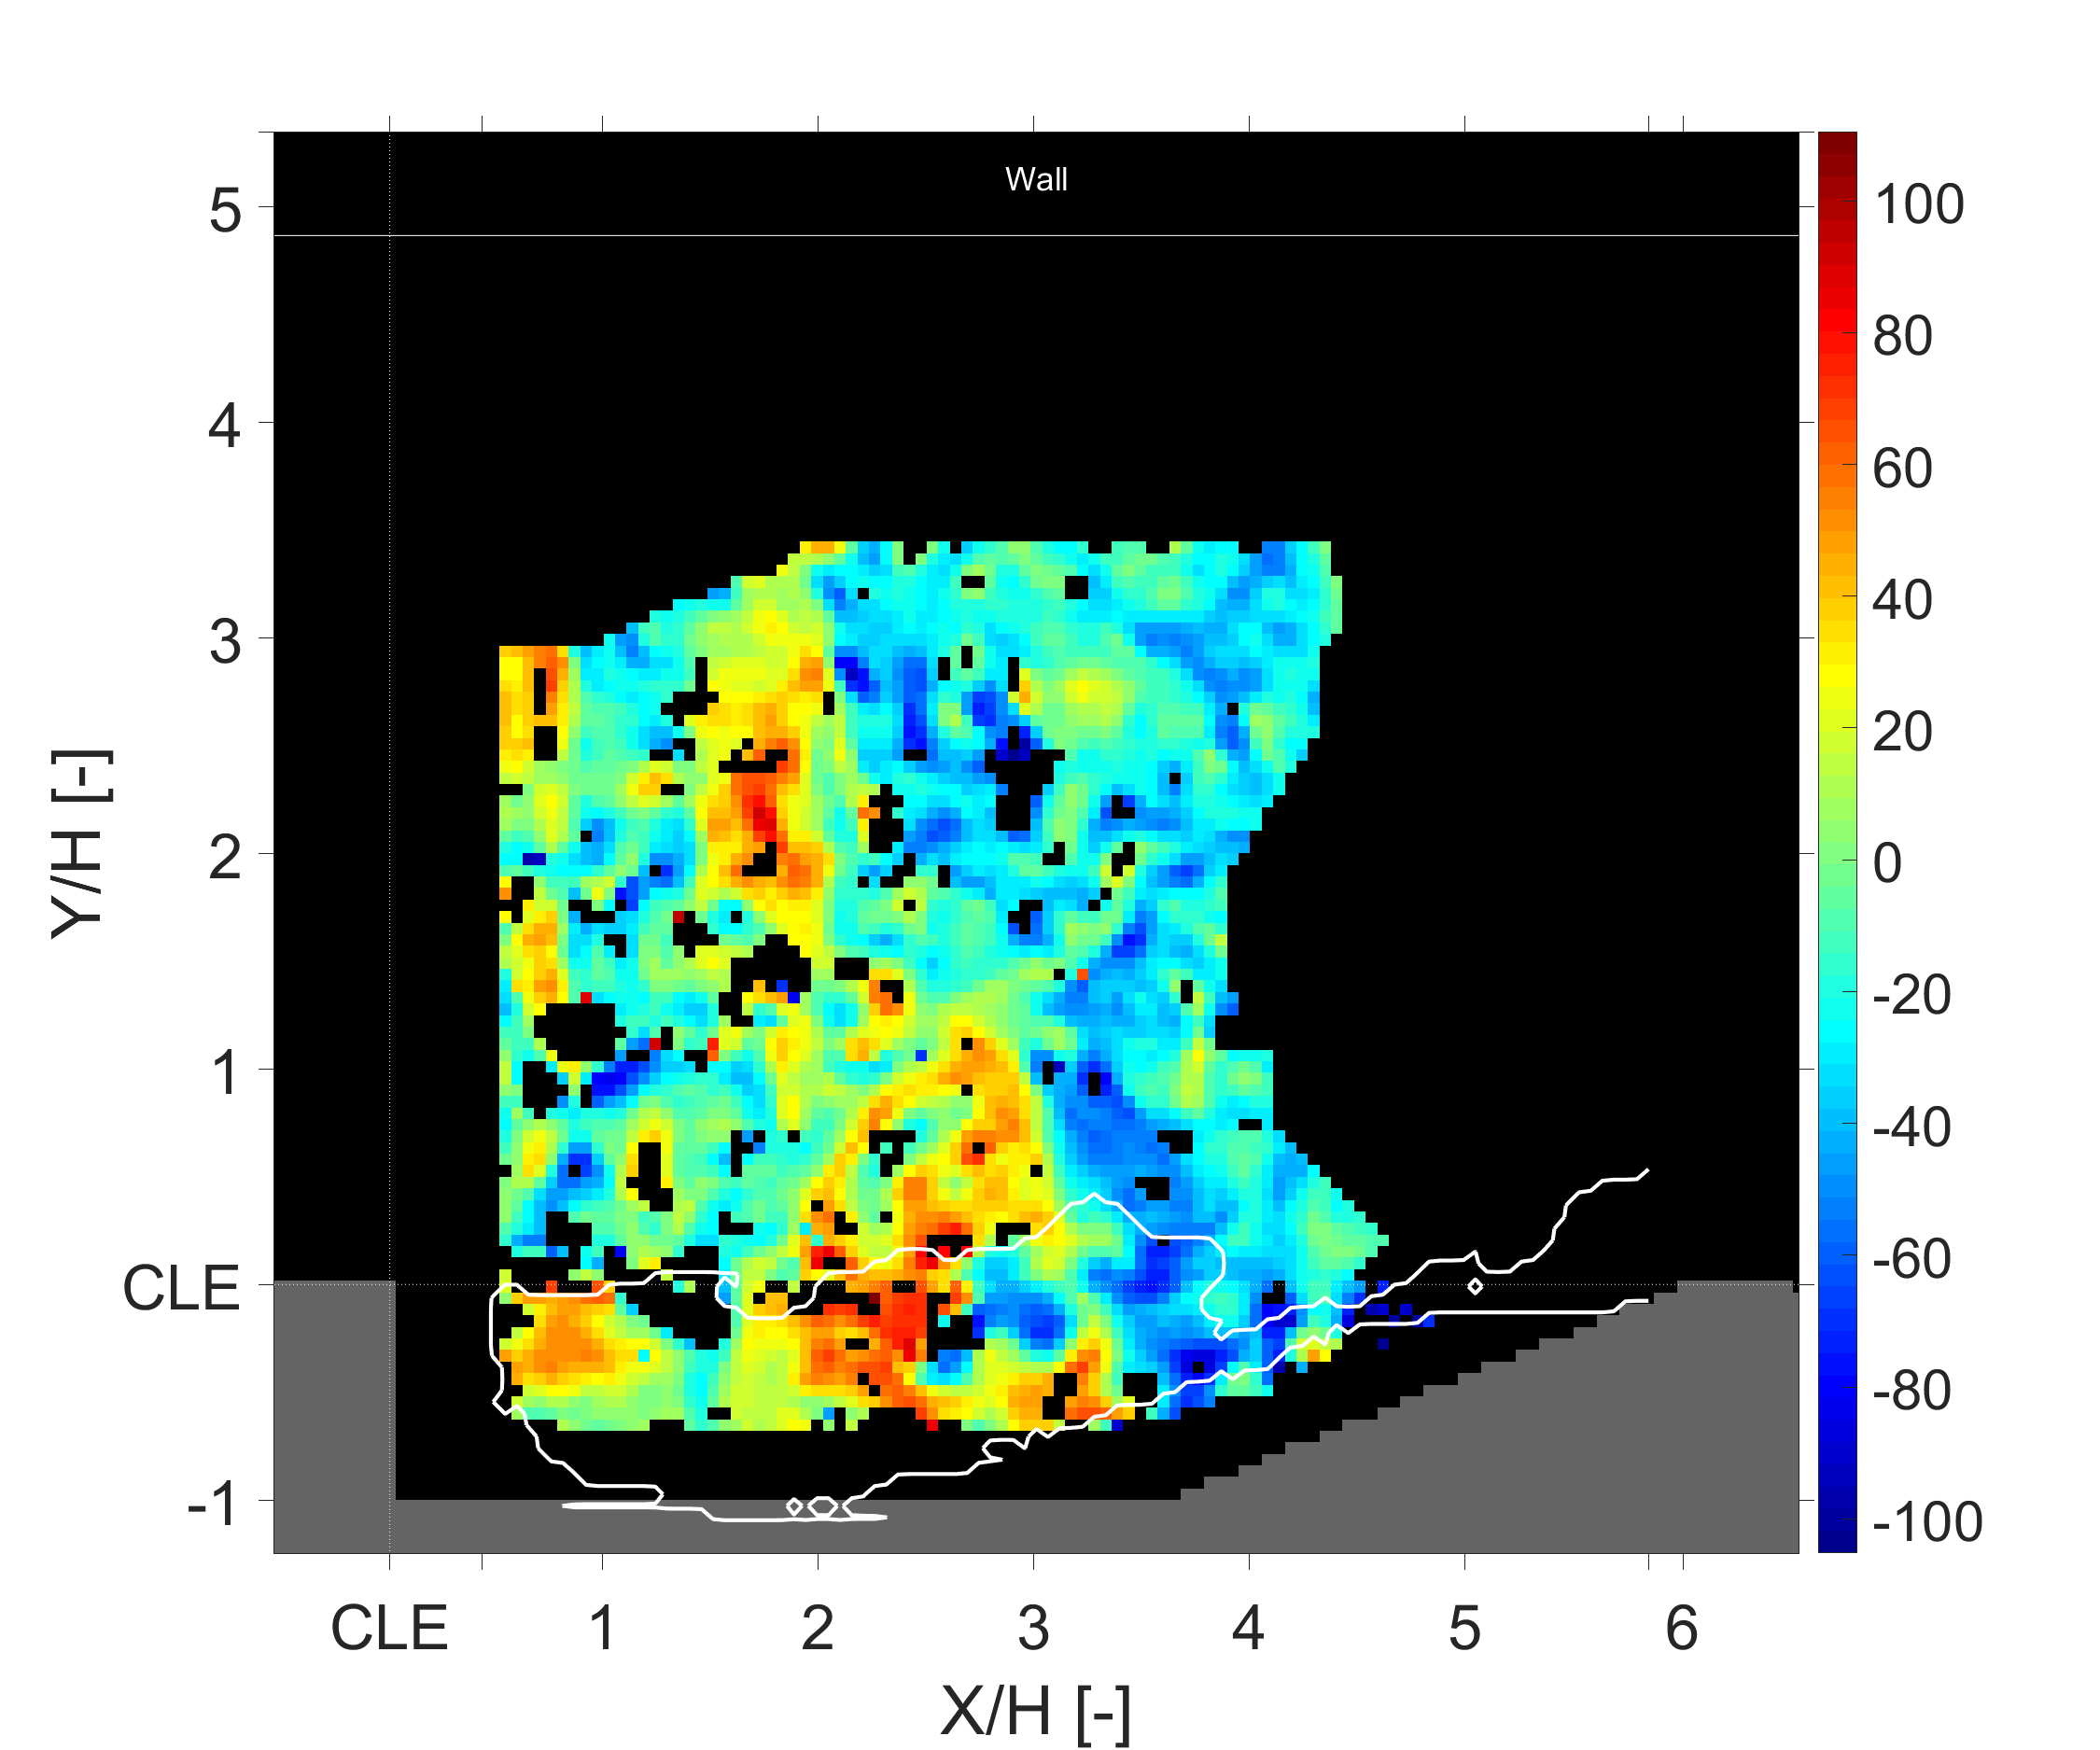
\includegraphics[height=2.5in, trim=0cm 0cm 0cm 0cm, clip]{figures/B1/combustion_instability/y/B1_Frame342_y}\hspace{0.5cm}}
% \subcaptionbox{State 4\label{fig:B1_Frame4y}}
%         {\hspace{0.5cm}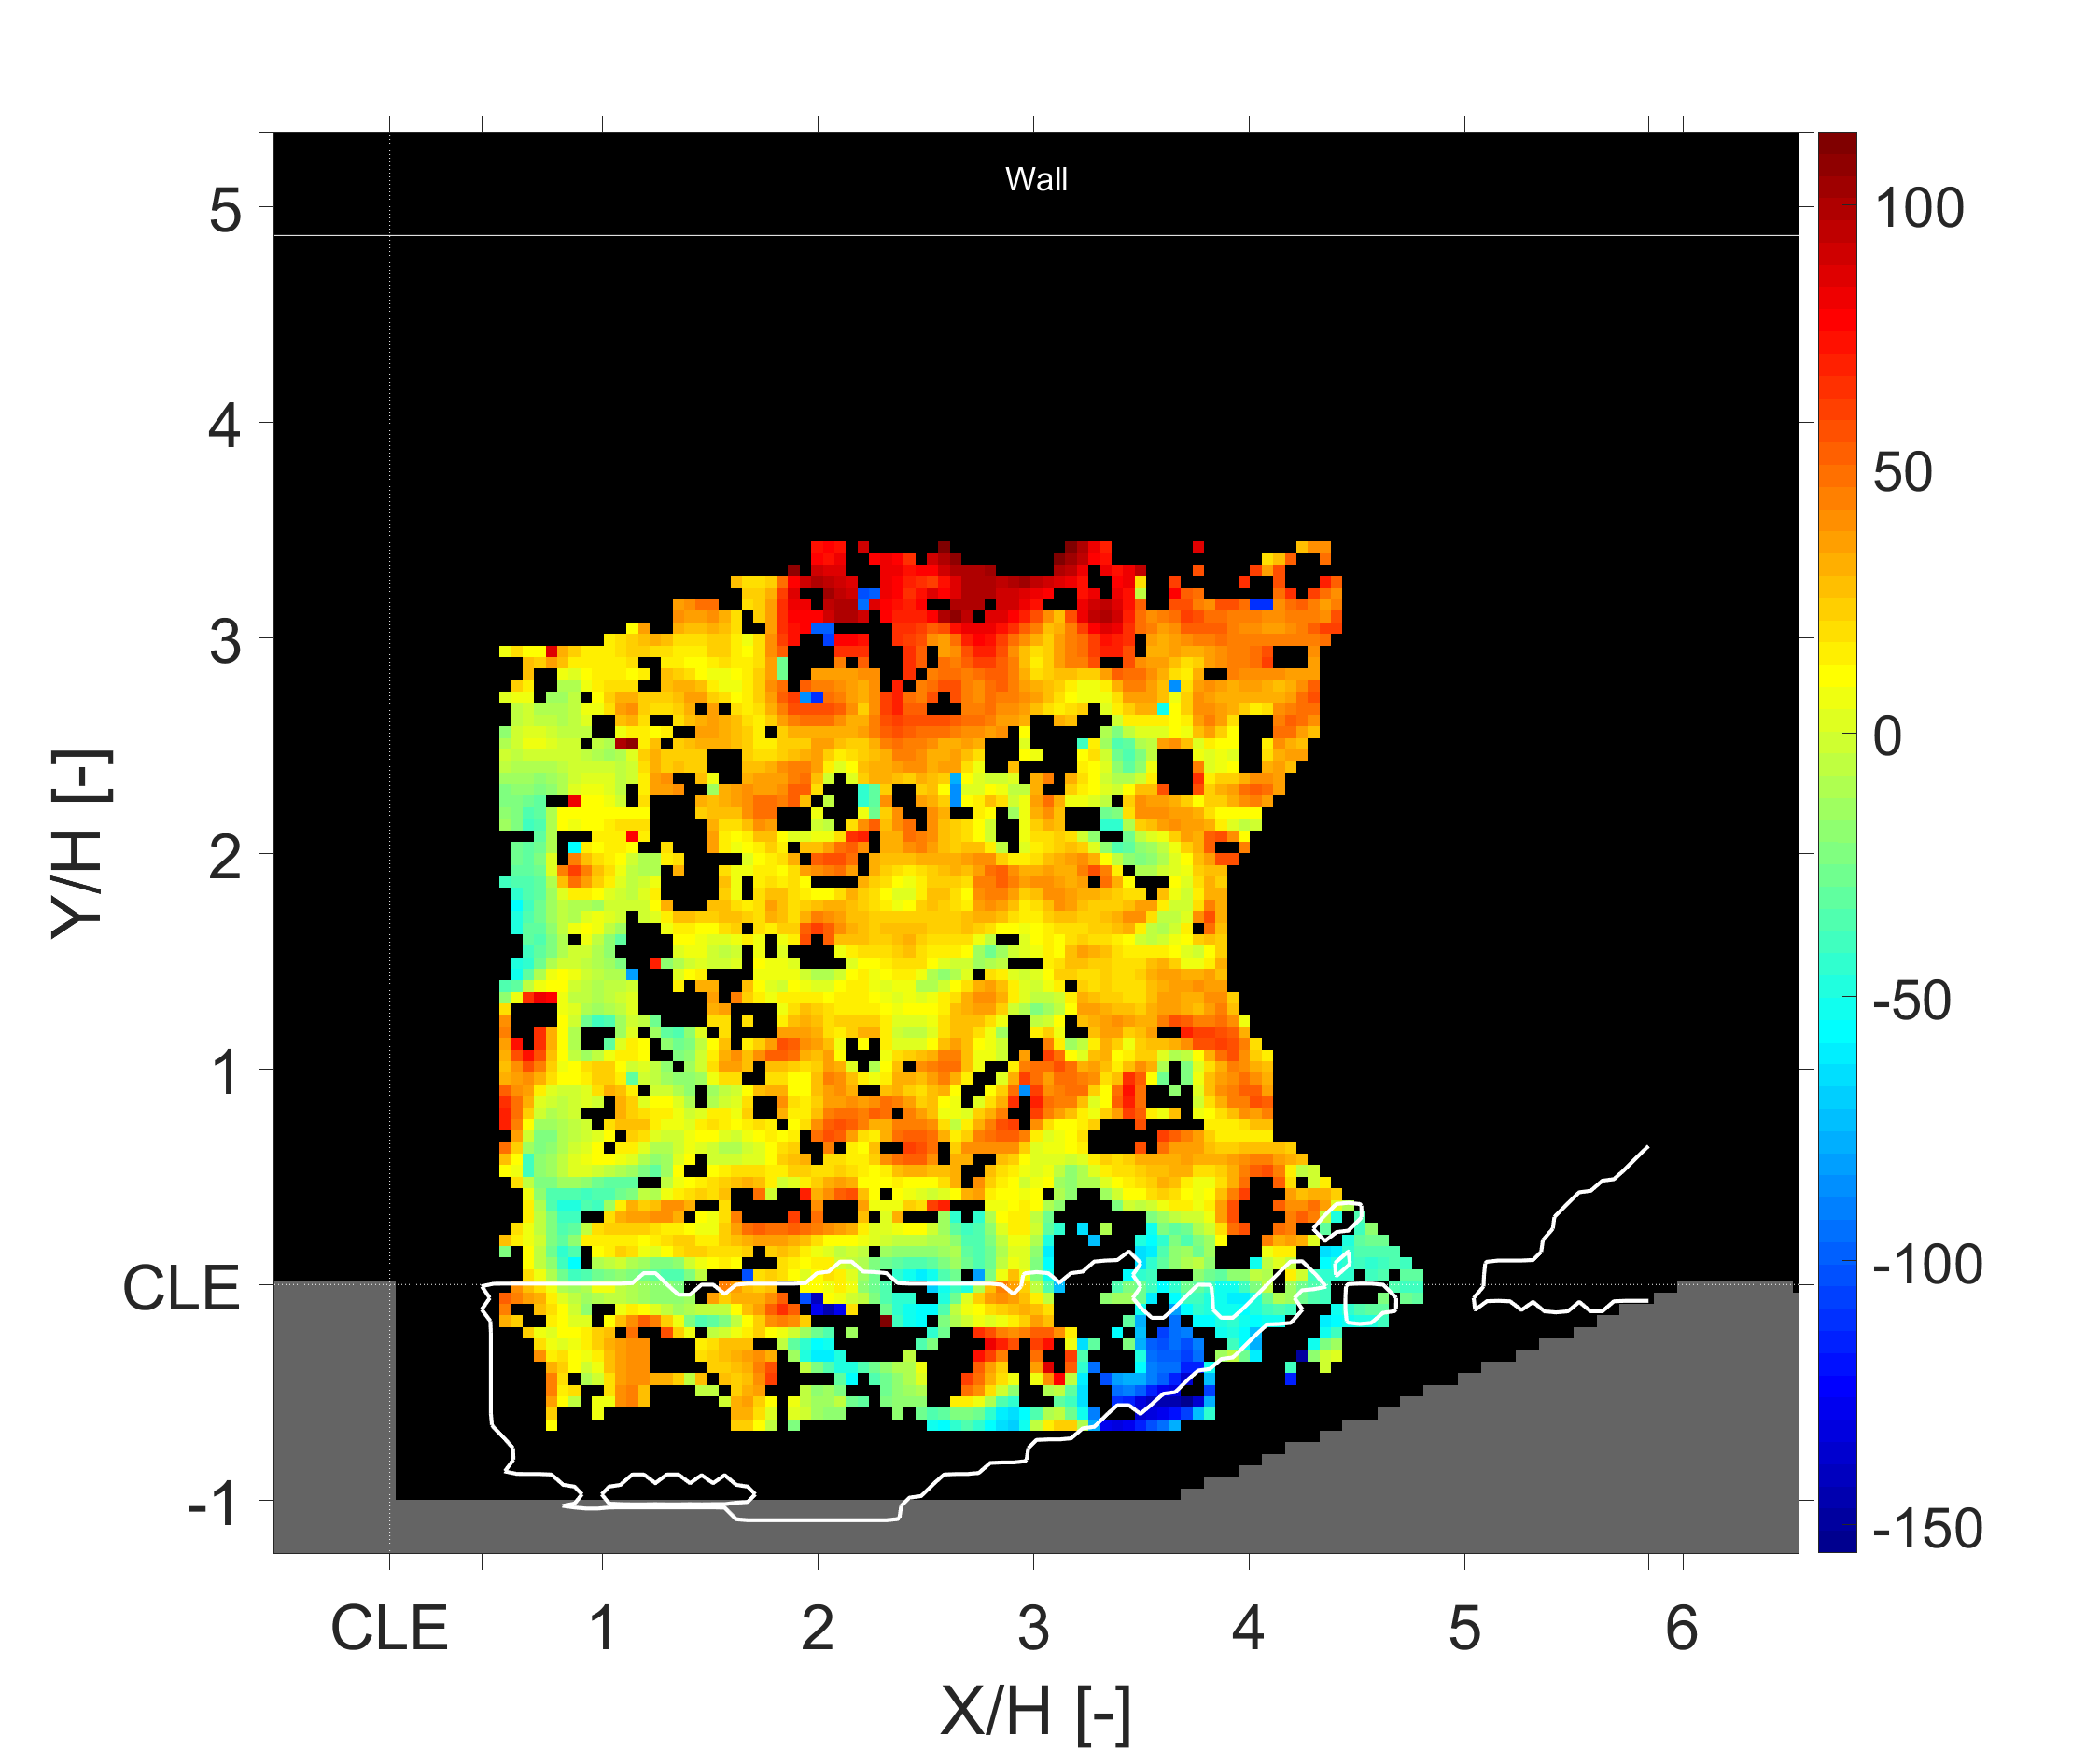
\includegraphics[height=2.5in, trim=0cm 0cm 0cm 0cm, clip]{figures/B1/combustion_instability/y/B1_Frame339_y}}
% \subcaptionbox{State 5\label{fig:B1_Frame5y}}
%         {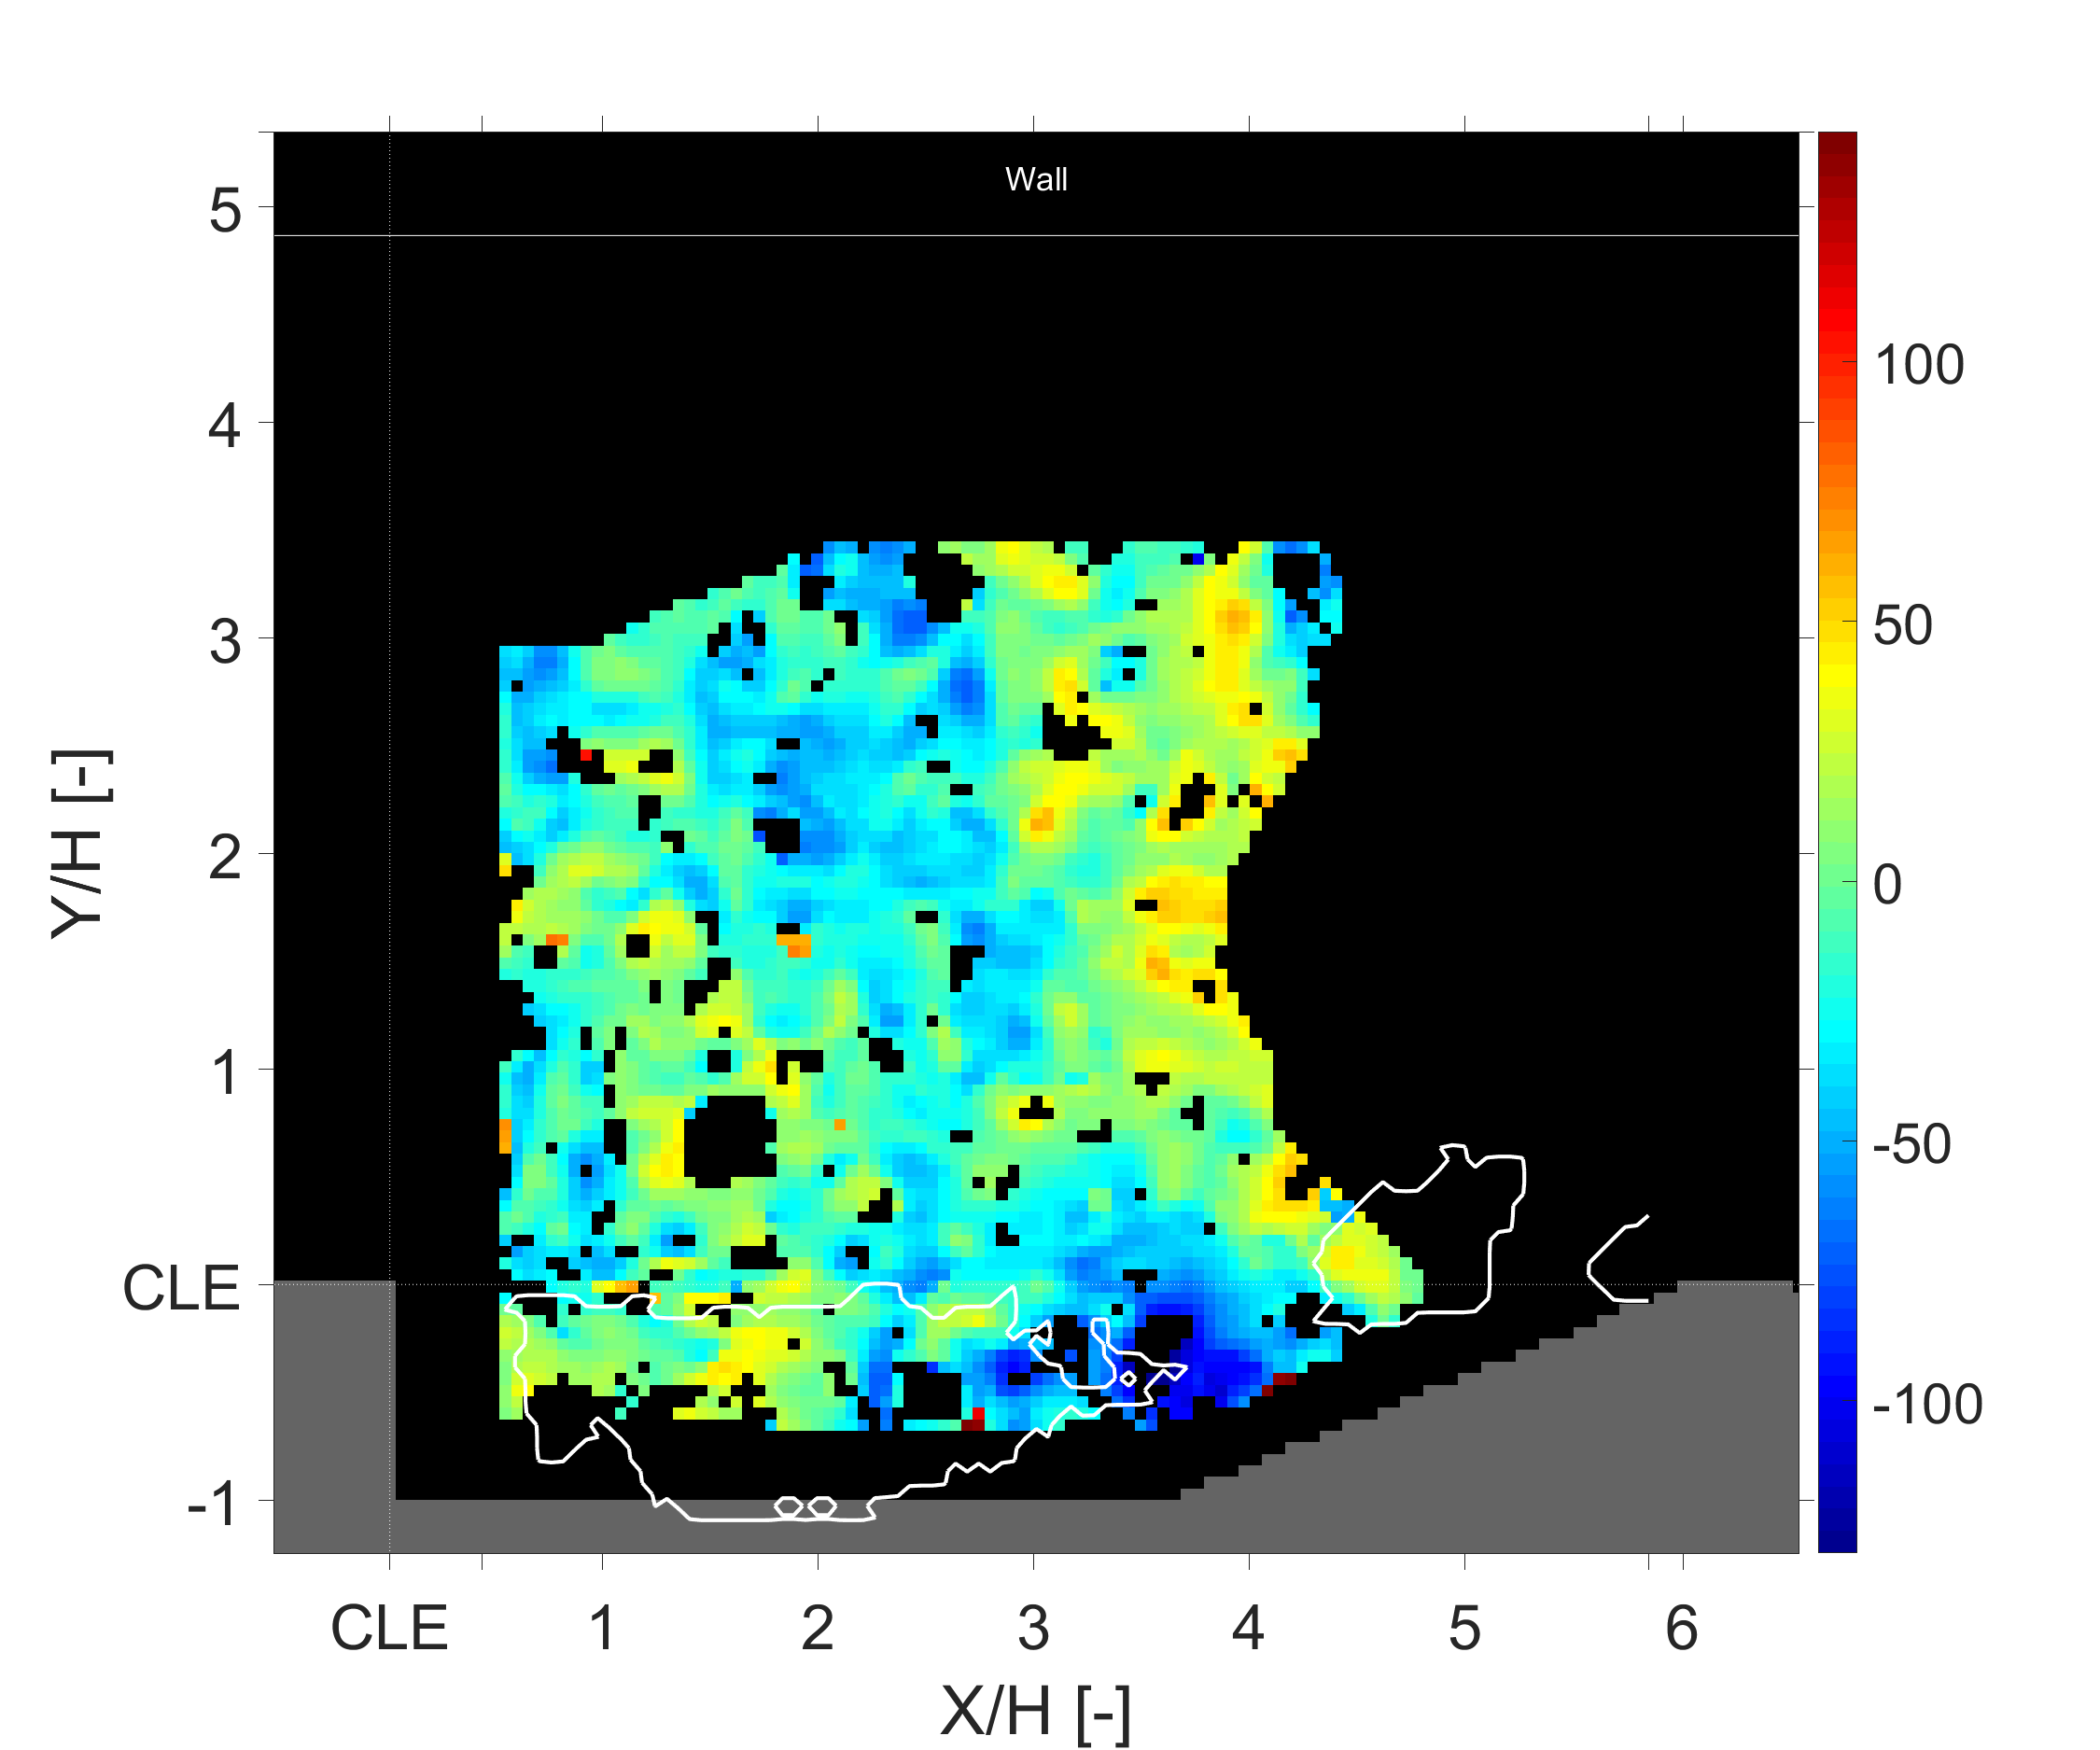
\includegraphics[height=2.5in, trim=0cm 0cm 0cm 0cm, clip]{figures/B1/combustion_instability/y/B1_Frame306_y.png}\hspace{0.5cm}}
%         \subcaptionbox{State 2 with duct velocities below average\label{fig:B1_Frame6y}}
%         {\hspace{0.5cm}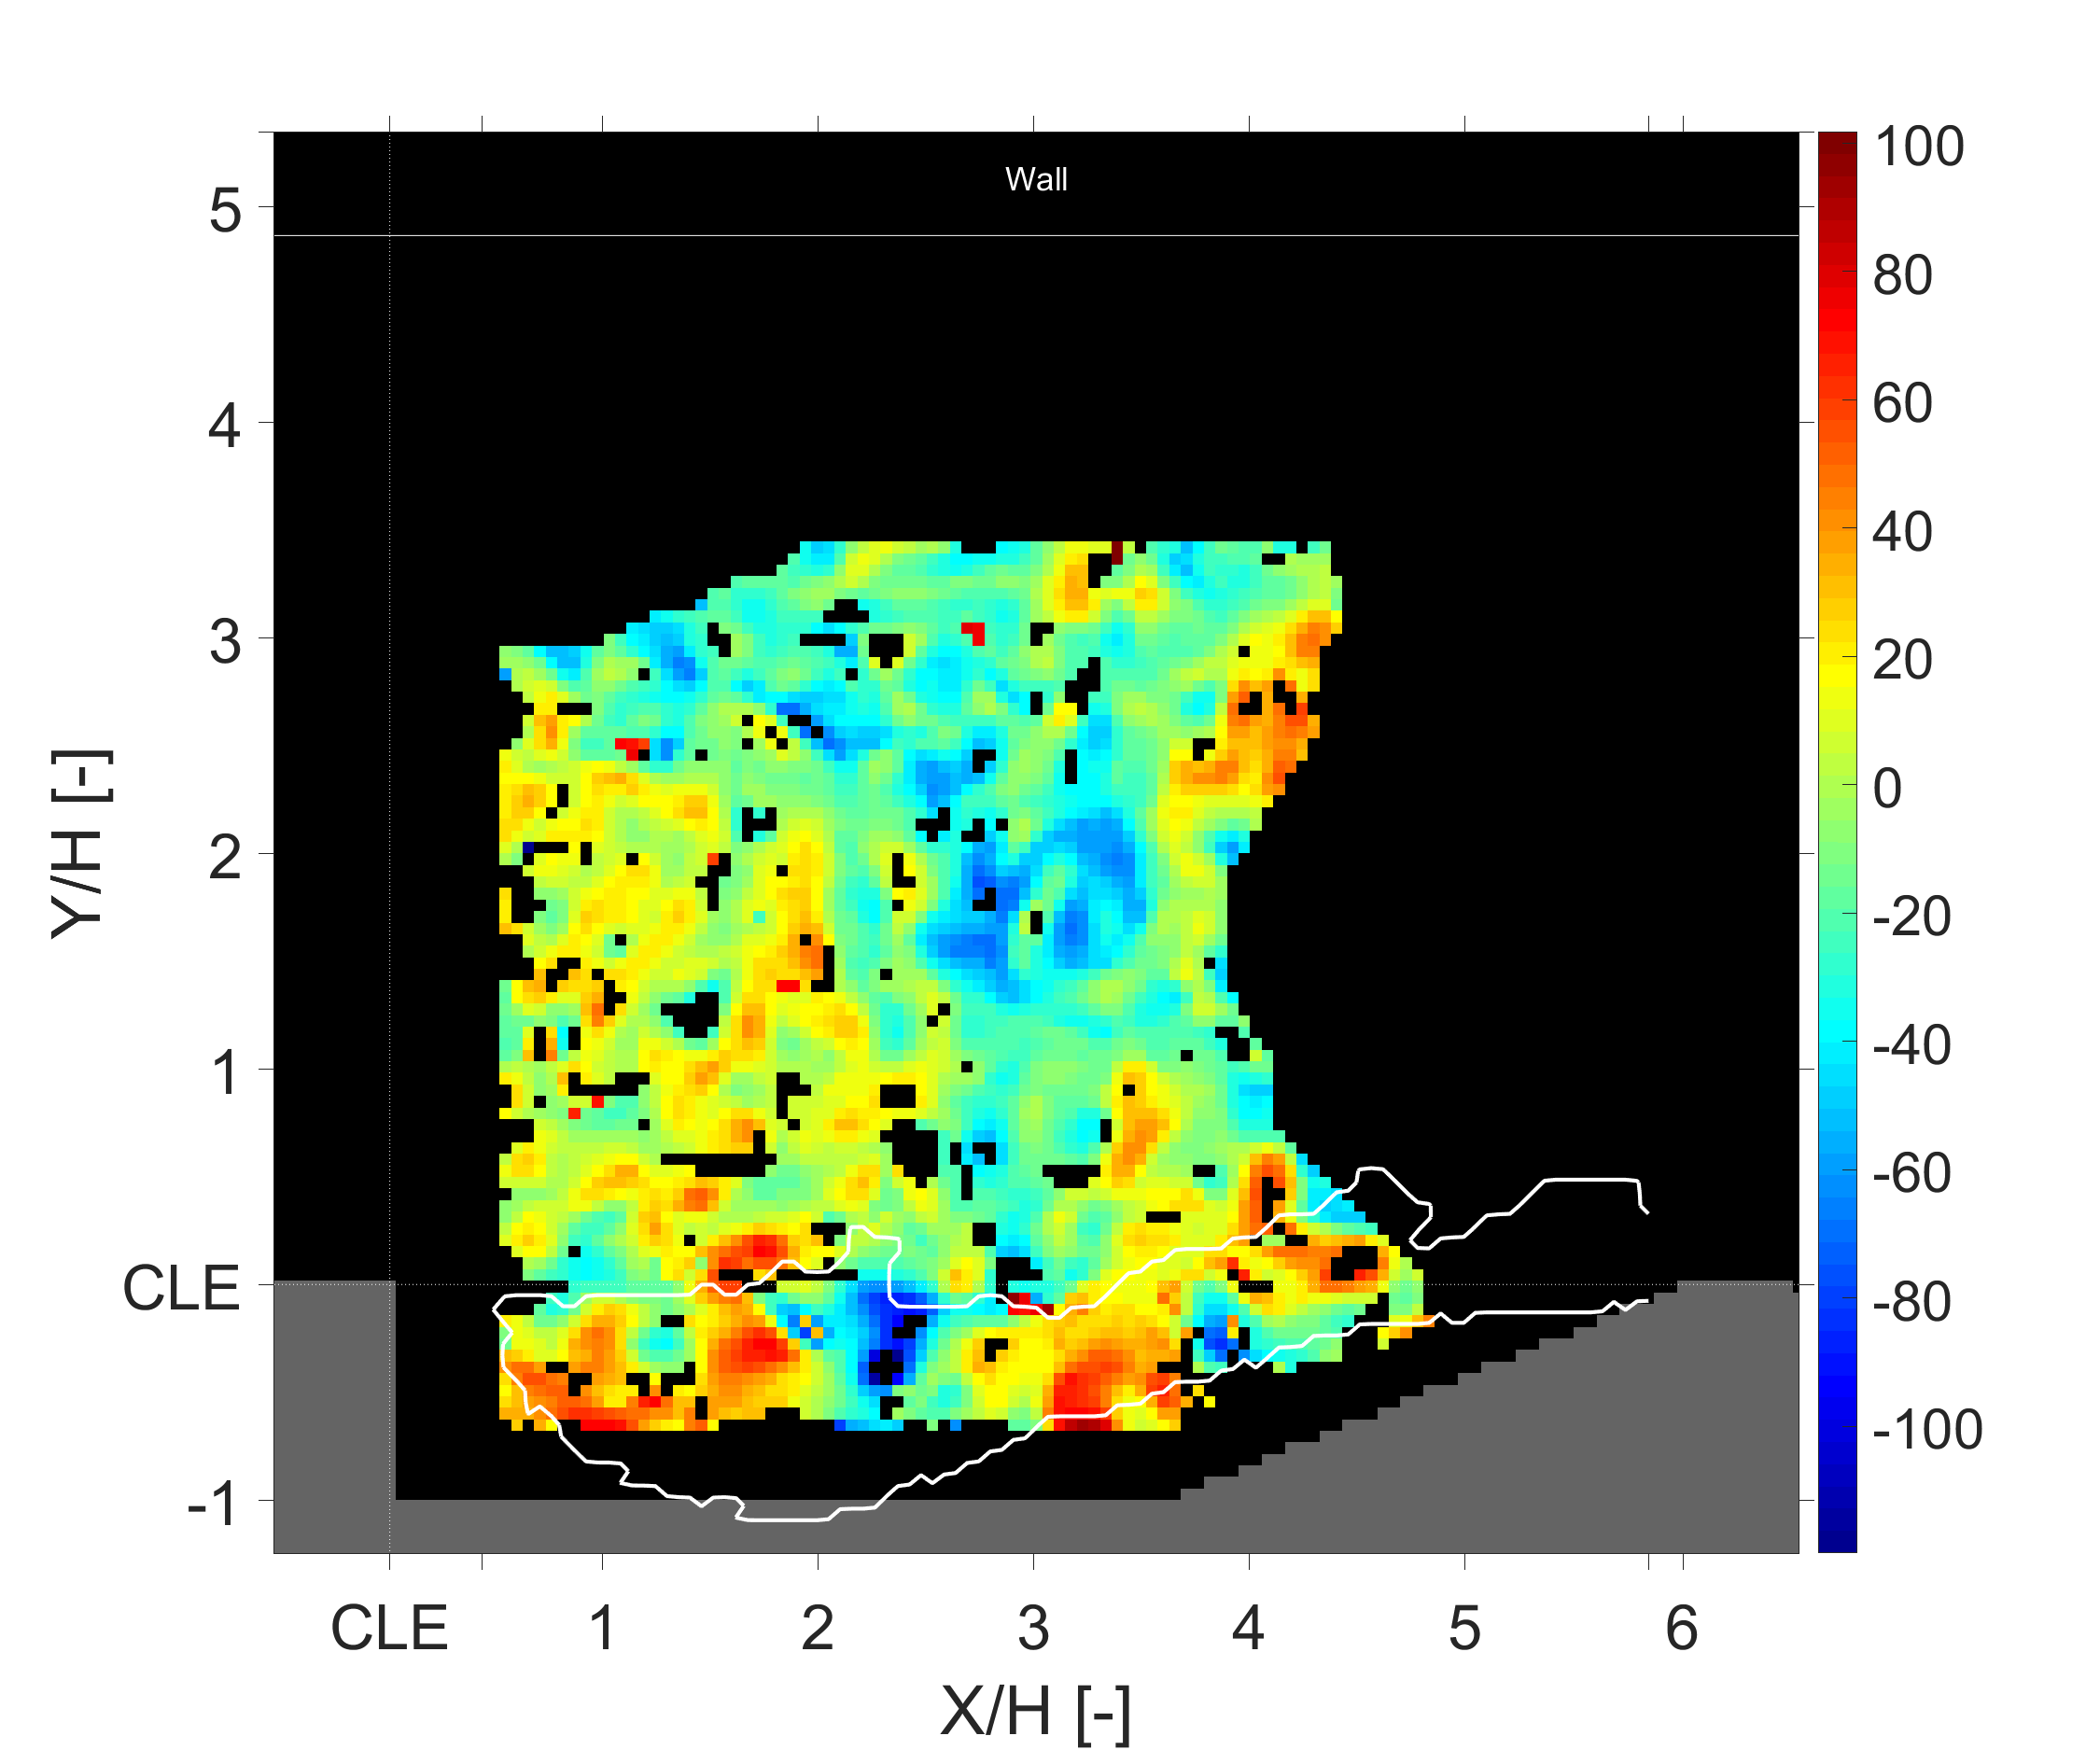
\includegraphics[height=2.5in, trim=0cm 0cm 0cm 0cm, clip]{figures/B1/combustion_instability/y/B1_Frame301_y}}
% \caption{$U_y$, select instantaneous PIV-PLIF frames.}\label{fig:ch3_inst_B1y}
% \end{figure}

\begin{figure}
\centering
\subcaptionbox{State 1\label{fig:B1_Frame1vec}}
      {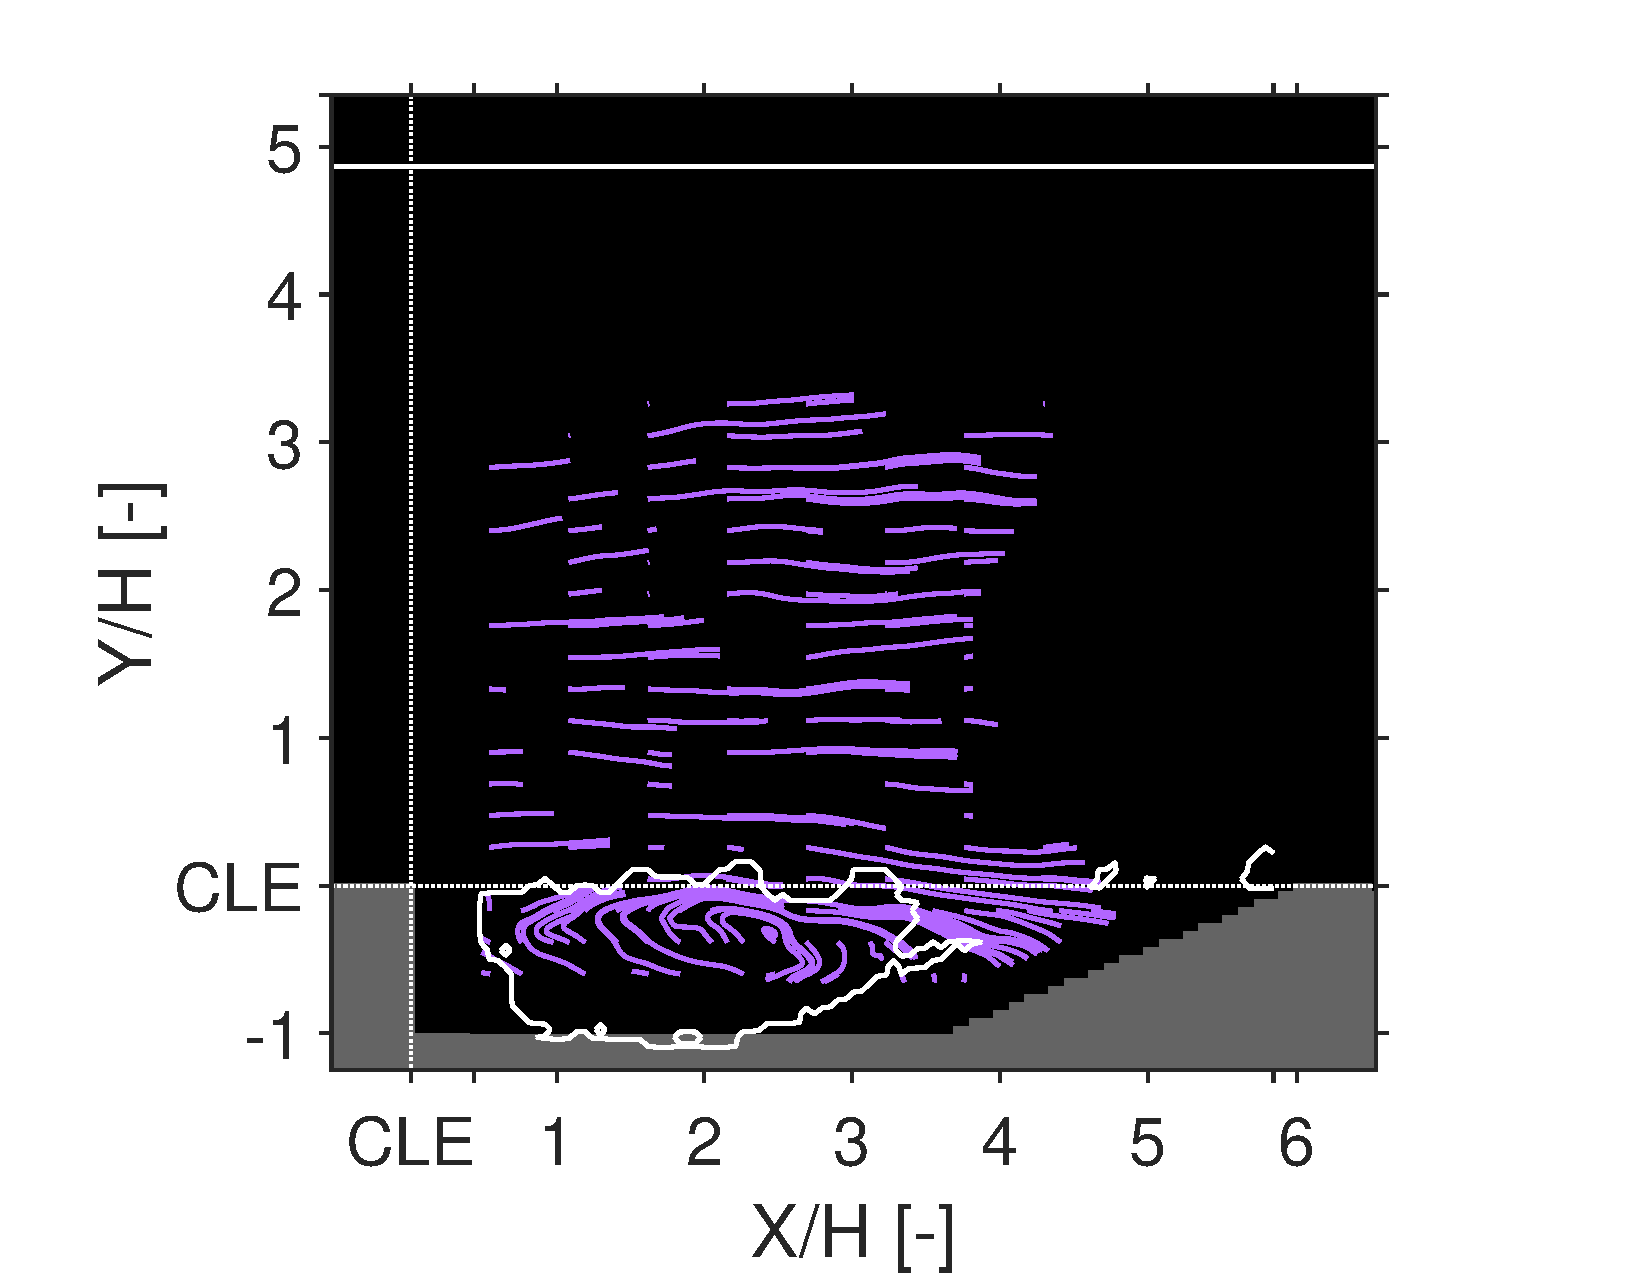
\includegraphics[width=3in,trim=0.35in 0 0.65in 0, clip]{figures/B1/combustion_instability/streamlines/B1_Frame331_v2.pdf}}
      \hspace{0.4cm}
\subcaptionbox{State 2\label{fig:B1_Frame2vec}}
                {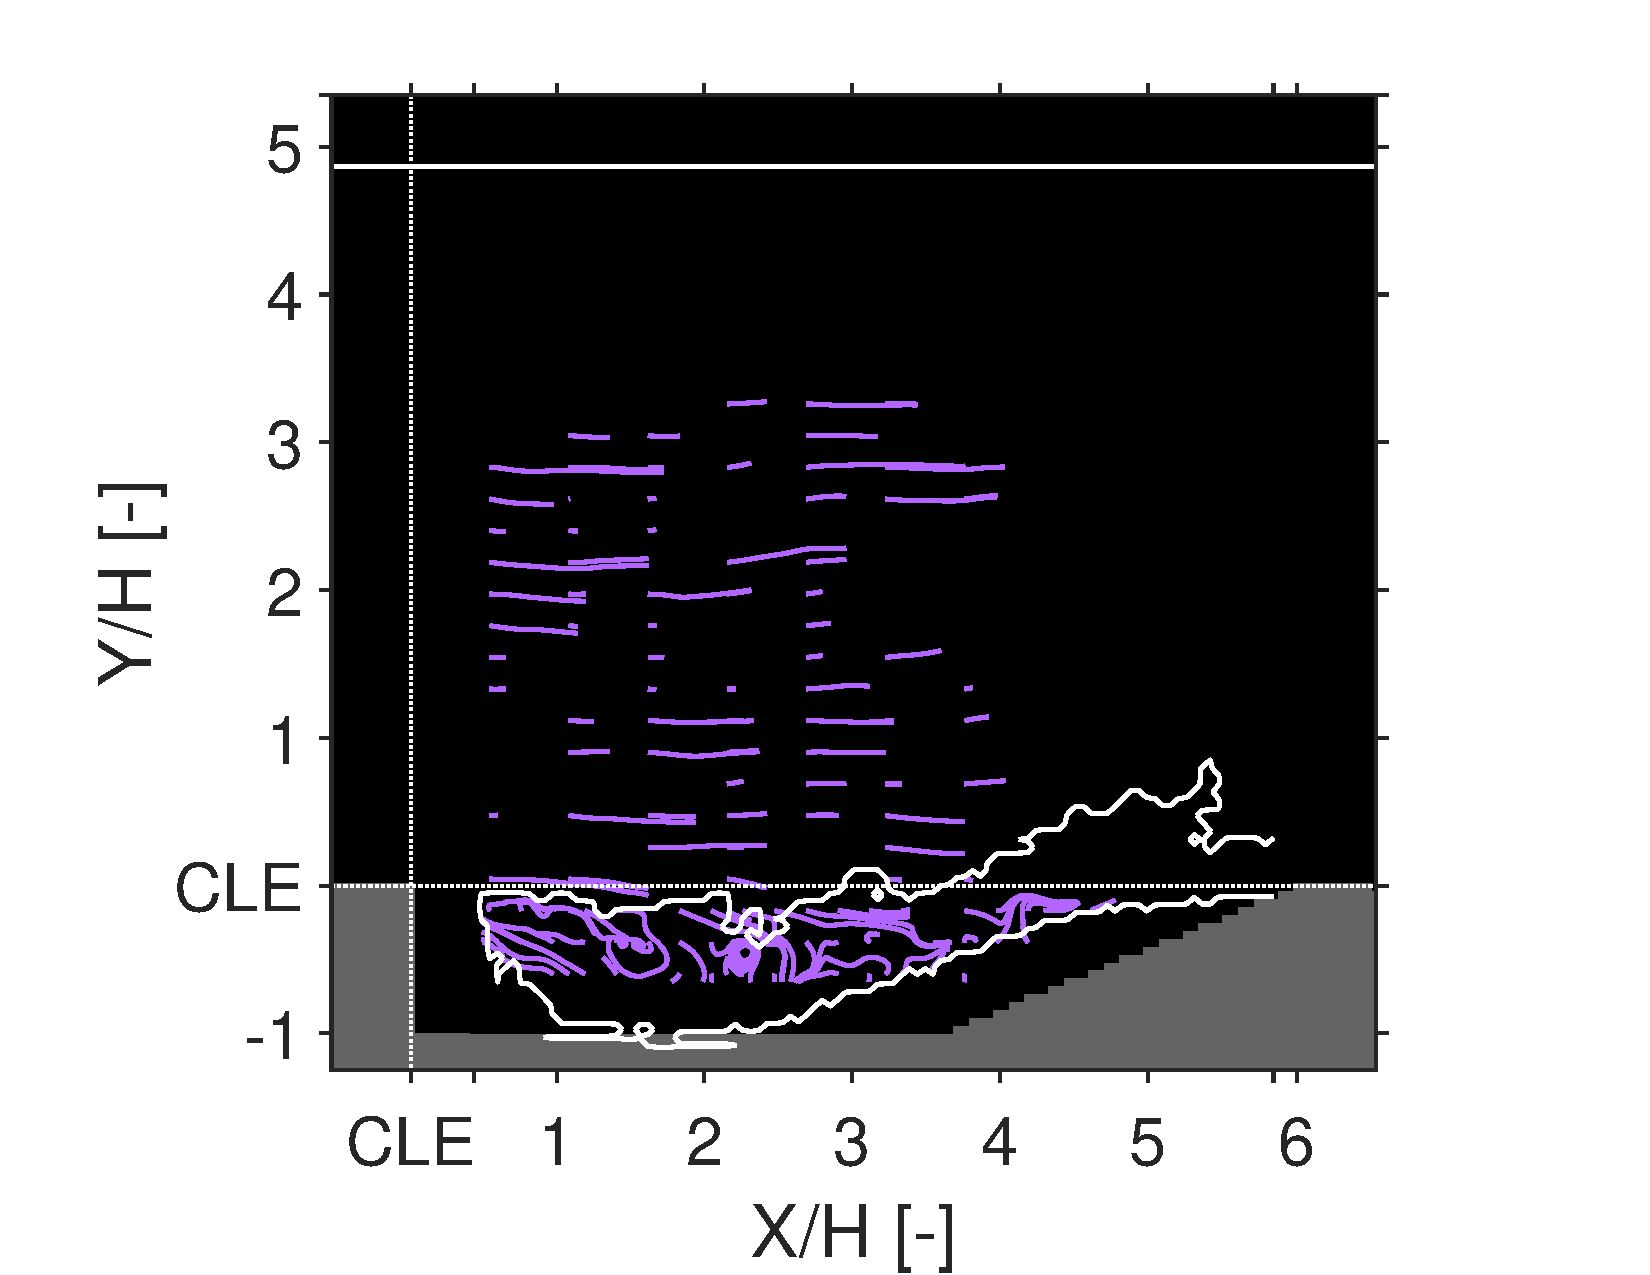
\includegraphics[width=3in,trim=0.35in 0 0.65in 0, clip]{figures/B1/combustion_instability/streamlines/B1_Frame329_v2.pdf}}
                \newline
\subcaptionbox{State 2'\label{fig:B1_Frame3vec}}
        {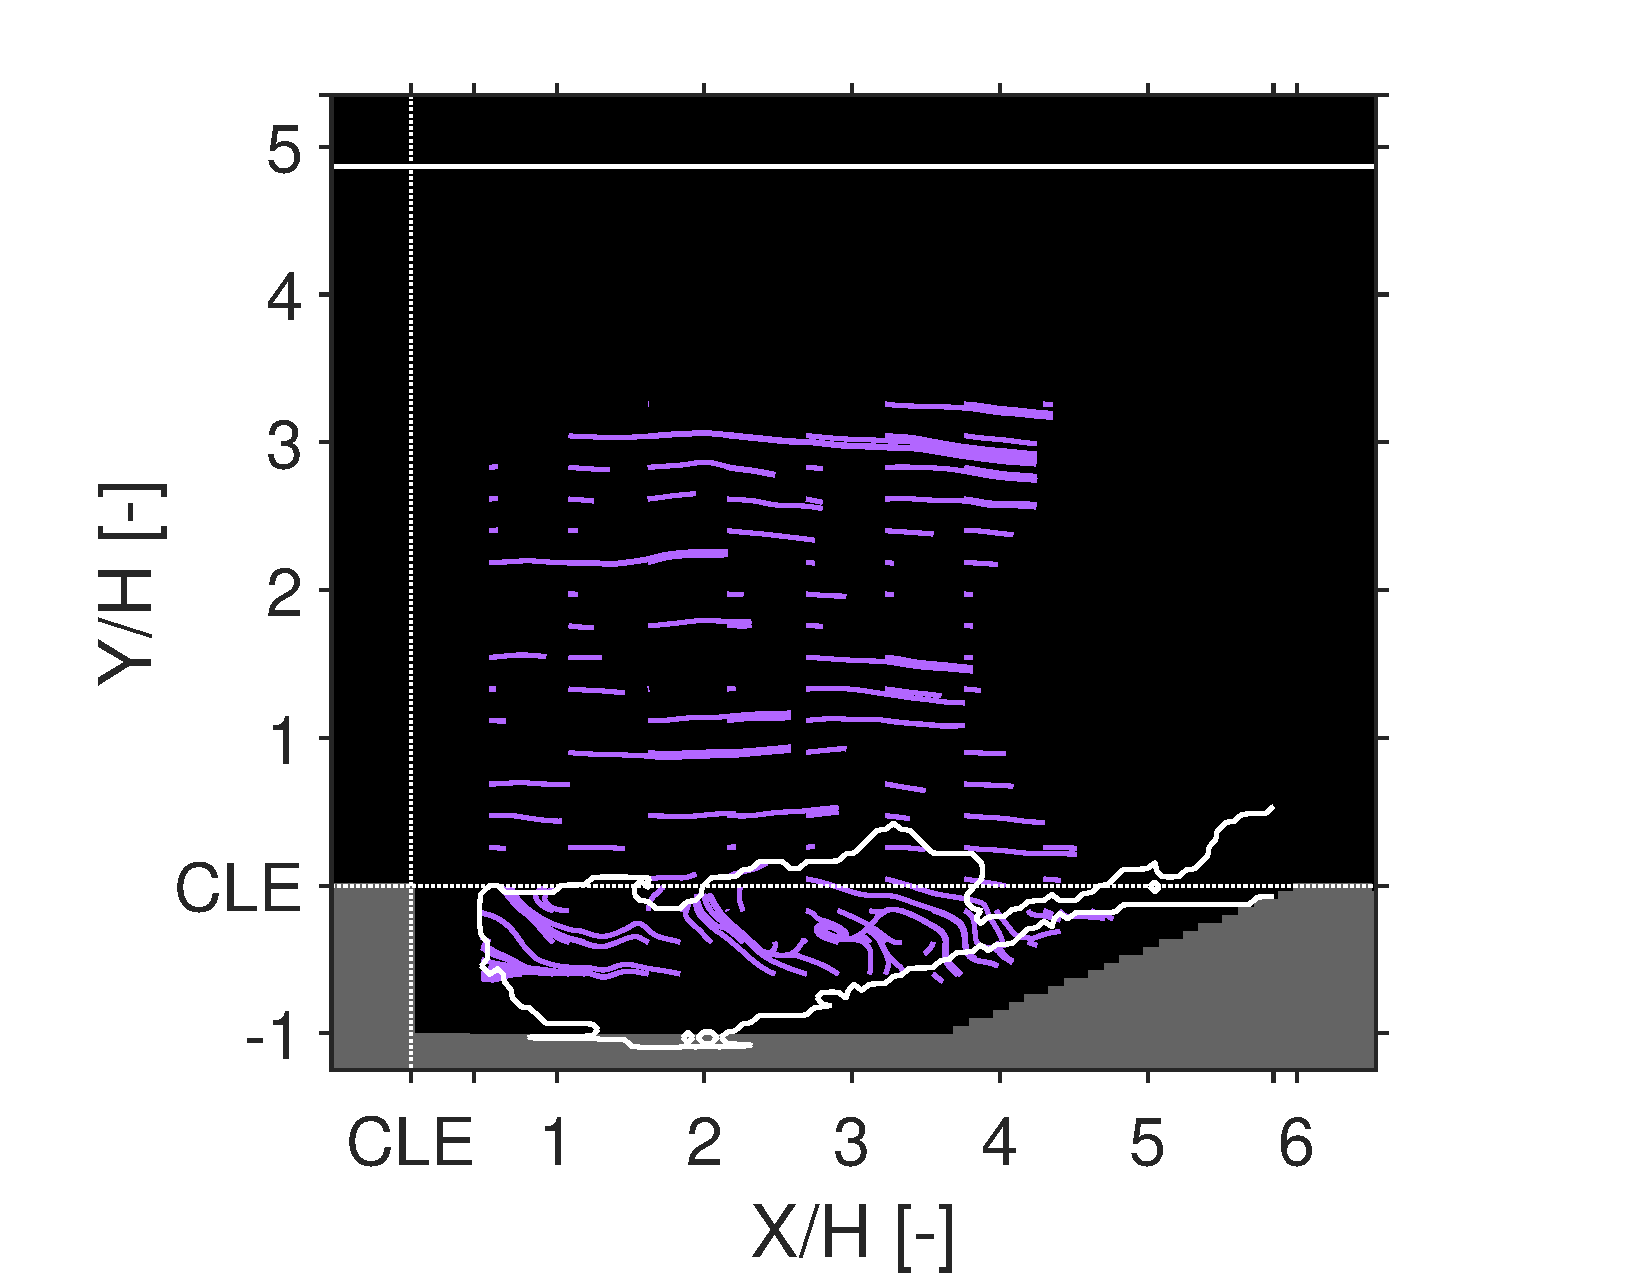
\includegraphics[width=3in,trim=0.35in 0 0.65in 0, clip]{figures/B1/combustion_instability/streamlines/B1_Frame342_v2.pdf}}
        \hspace{0.4cm}
\subcaptionbox{State 3\label{fig:B1_Frame4vec}}
                {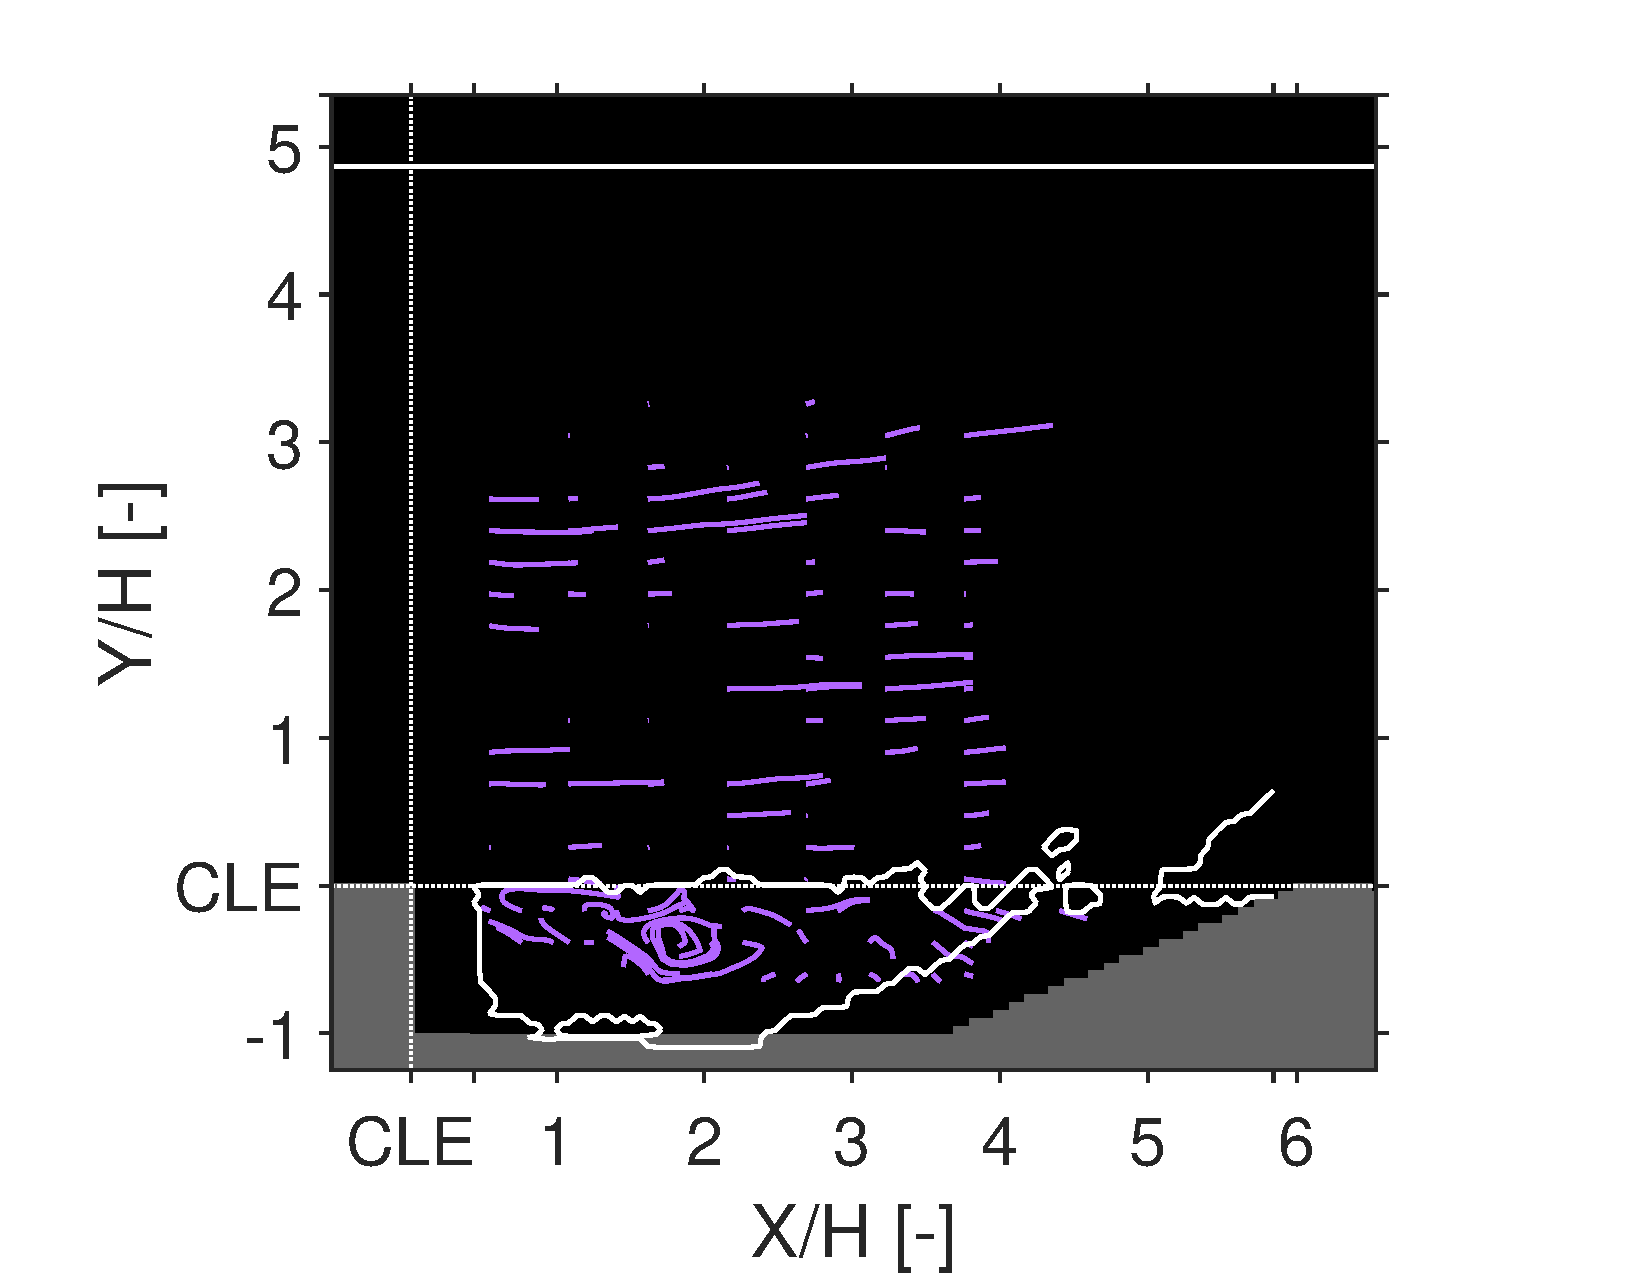
\includegraphics[width=3in,trim=0.35in 0 0.65in 0, clip]{figures/B1/combustion_instability/streamlines/B1_Frame339_v2.pdf}}
                \newline
 \subcaptionbox{State 3'\label{fig:B1_Frame5vec}}
         {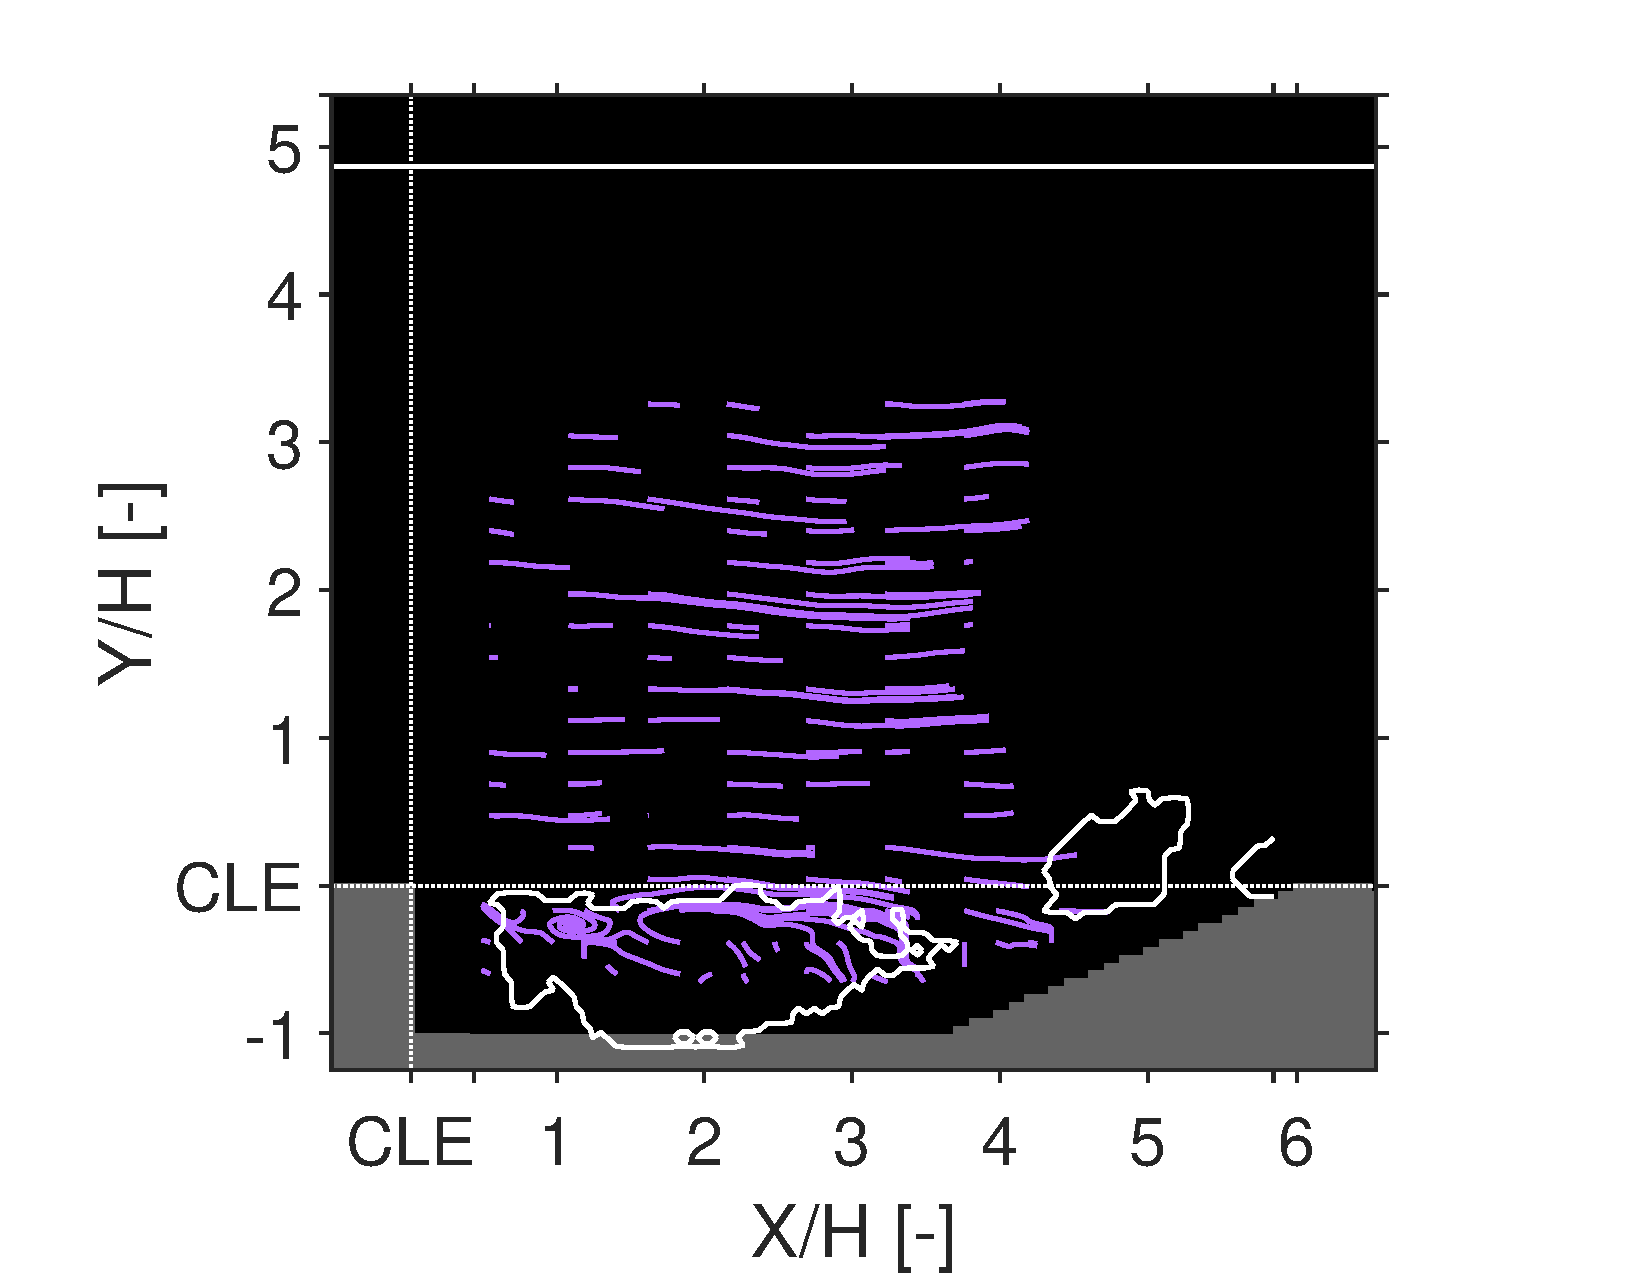
\includegraphics[width=3in,trim=0.35in 0 0.65in 0, clip]{figures/B1/combustion_instability/streamlines/B1_Frame306_v2.pdf}}
         \hspace{0.4cm}
        \subcaptionbox{State 2 with duct velocities below average\label{fig:B1_Frame6vec}}
                {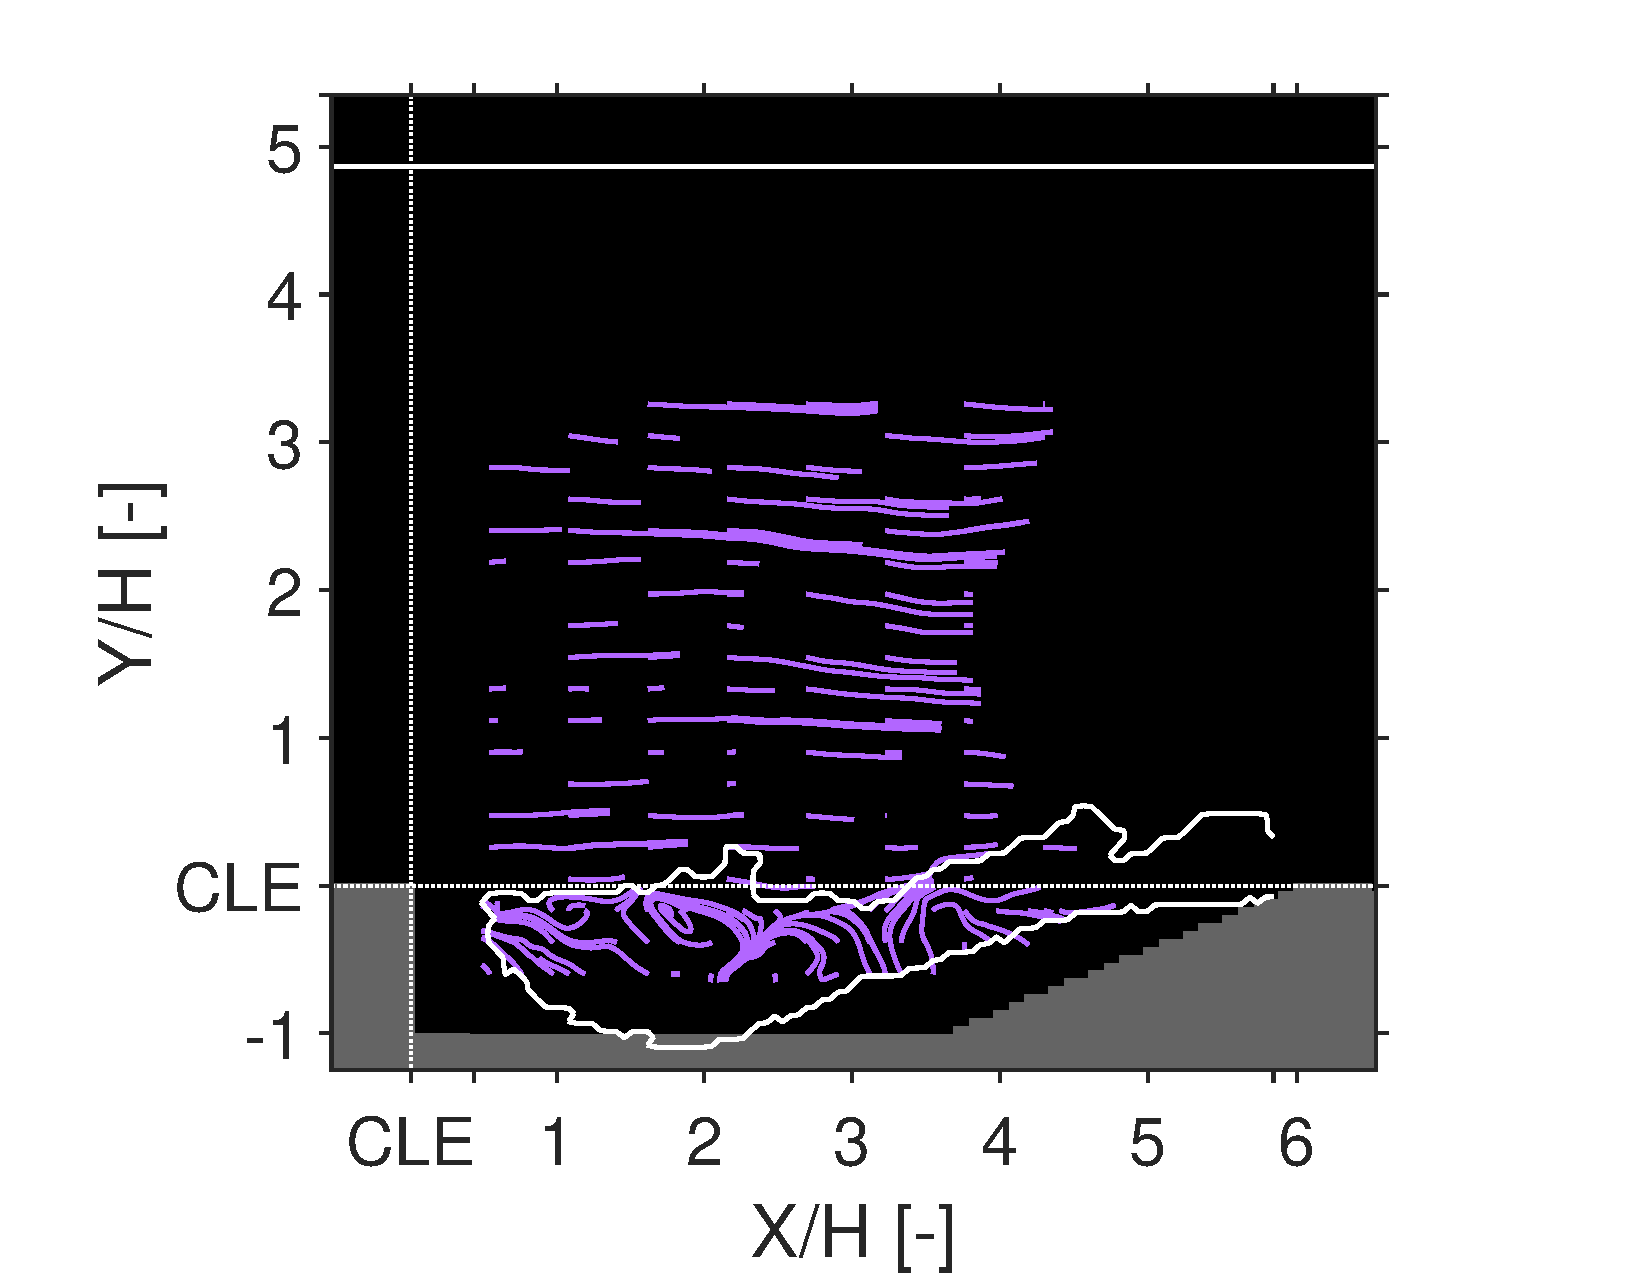
\includegraphics[width=3in,trim=0.35in 0 0.65in 0, clip]{figures/B1/combustion_instability/streamlines/B1_Frame301_v2.pdf}}
\caption{Streamlines, select instantaneous PIV-PLIF frames.}\label{fig:ch3_inst_B1vec}
\end{figure}

For all three states, the cavity flame closely abides by the shear layer, wrinkles around the shear-layer eddies (identified by high swirling strength values in Fig. \ref{fig:ch3_inst_ST}), and is either continuous or split into two regions. The shear-layer eddies serve to exchange combustion radicals generated in the cavity with the fresh premixed flow from the duct. These eddies are of similar size to eddies found in the free stream (Fig. \ref{fig:ch3_inst_ST}). In addition, large scale free stream fluctuations are observed in the streamlines and vectors of Figs. \ref{fig:ch3_inst_B1} and \ref{fig:ch3_inst_ST}. Measurements with the shear layer impinging on the cavity ramp are correlated with a negative transverse velocity in the free stream flow close to the cavity. The above observations suggest that spatial scales on the order of $H$ in the cavity flame are coupled with the free stream scales.

\begin{figure}
\centering
\subcaptionbox{State 1\label{fig:B1_R1_ST}}
        {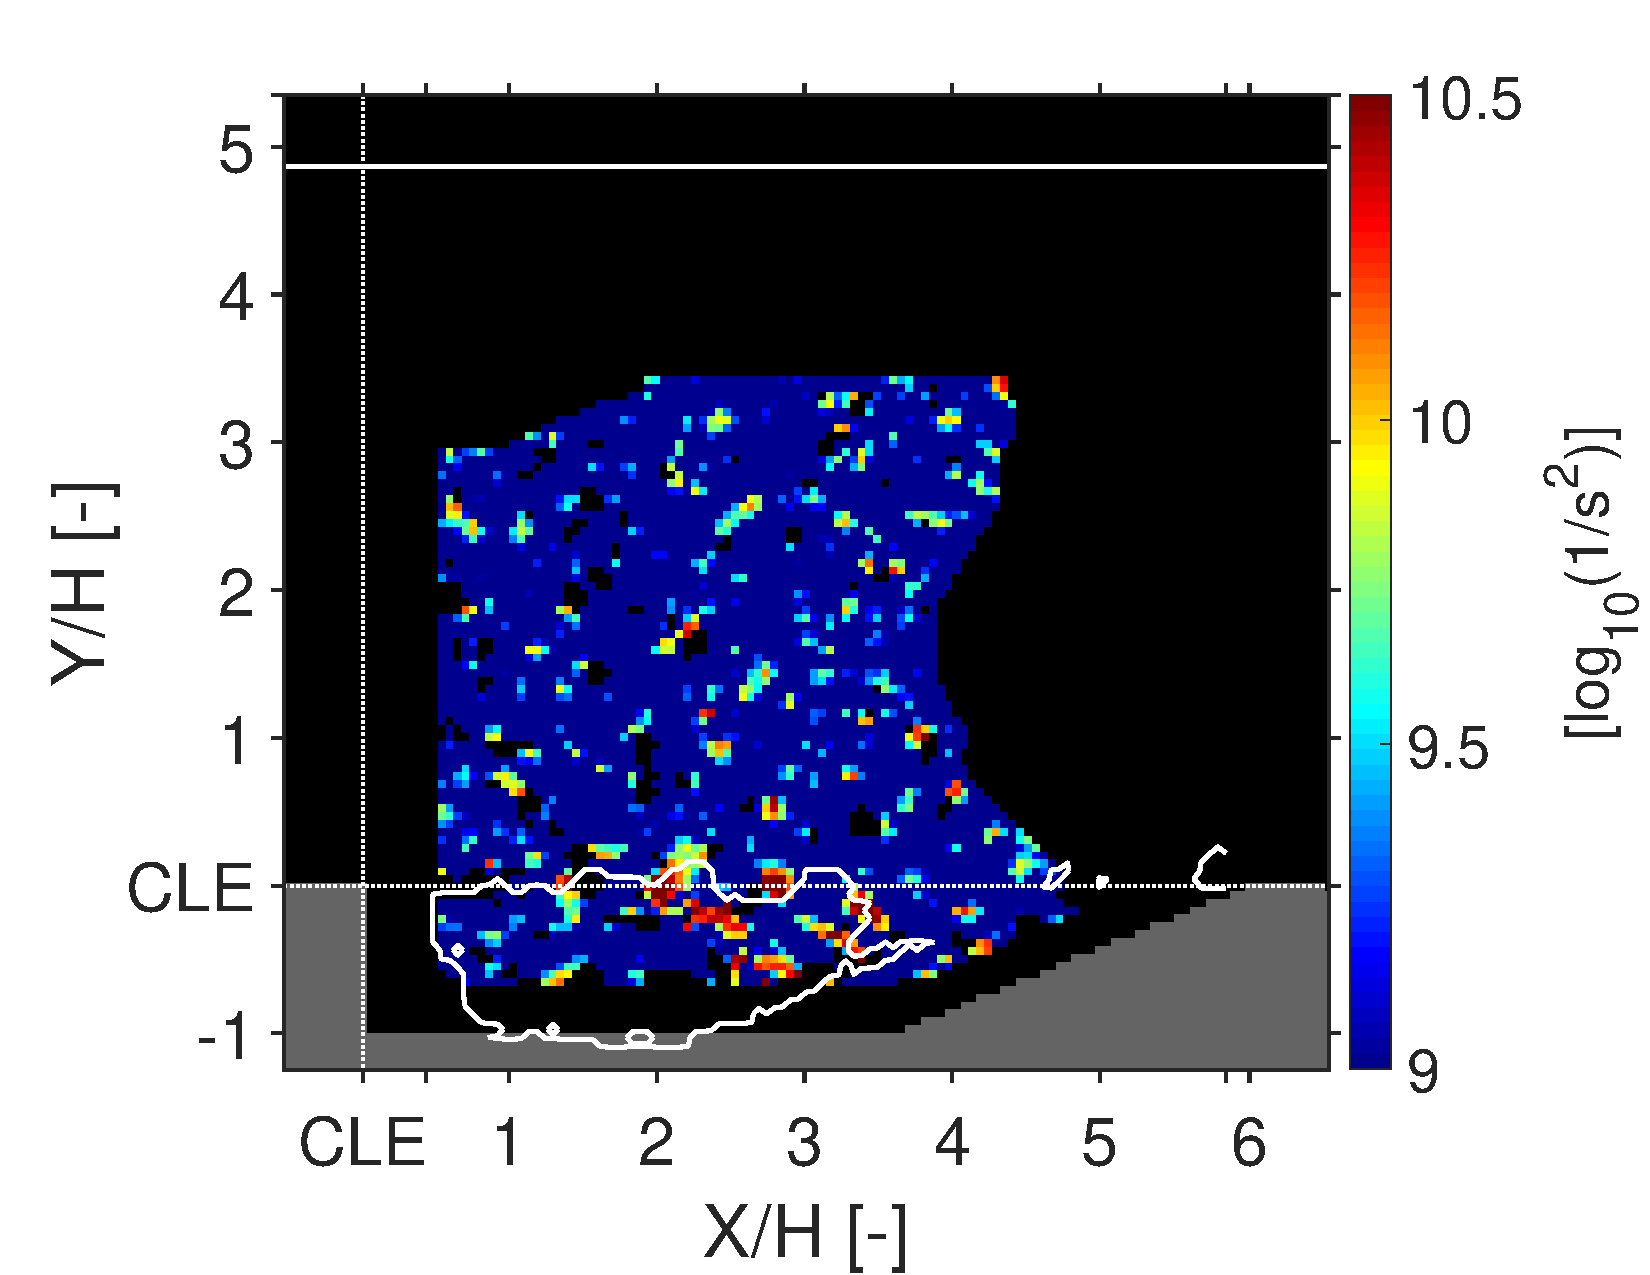
\includegraphics[width=3.25in]{figures/B1/B1_swirling_strength/B1_Frame331.pdf}} \\
\subcaptionbox{State 2\label{fig:B1_R2_ST}}{
        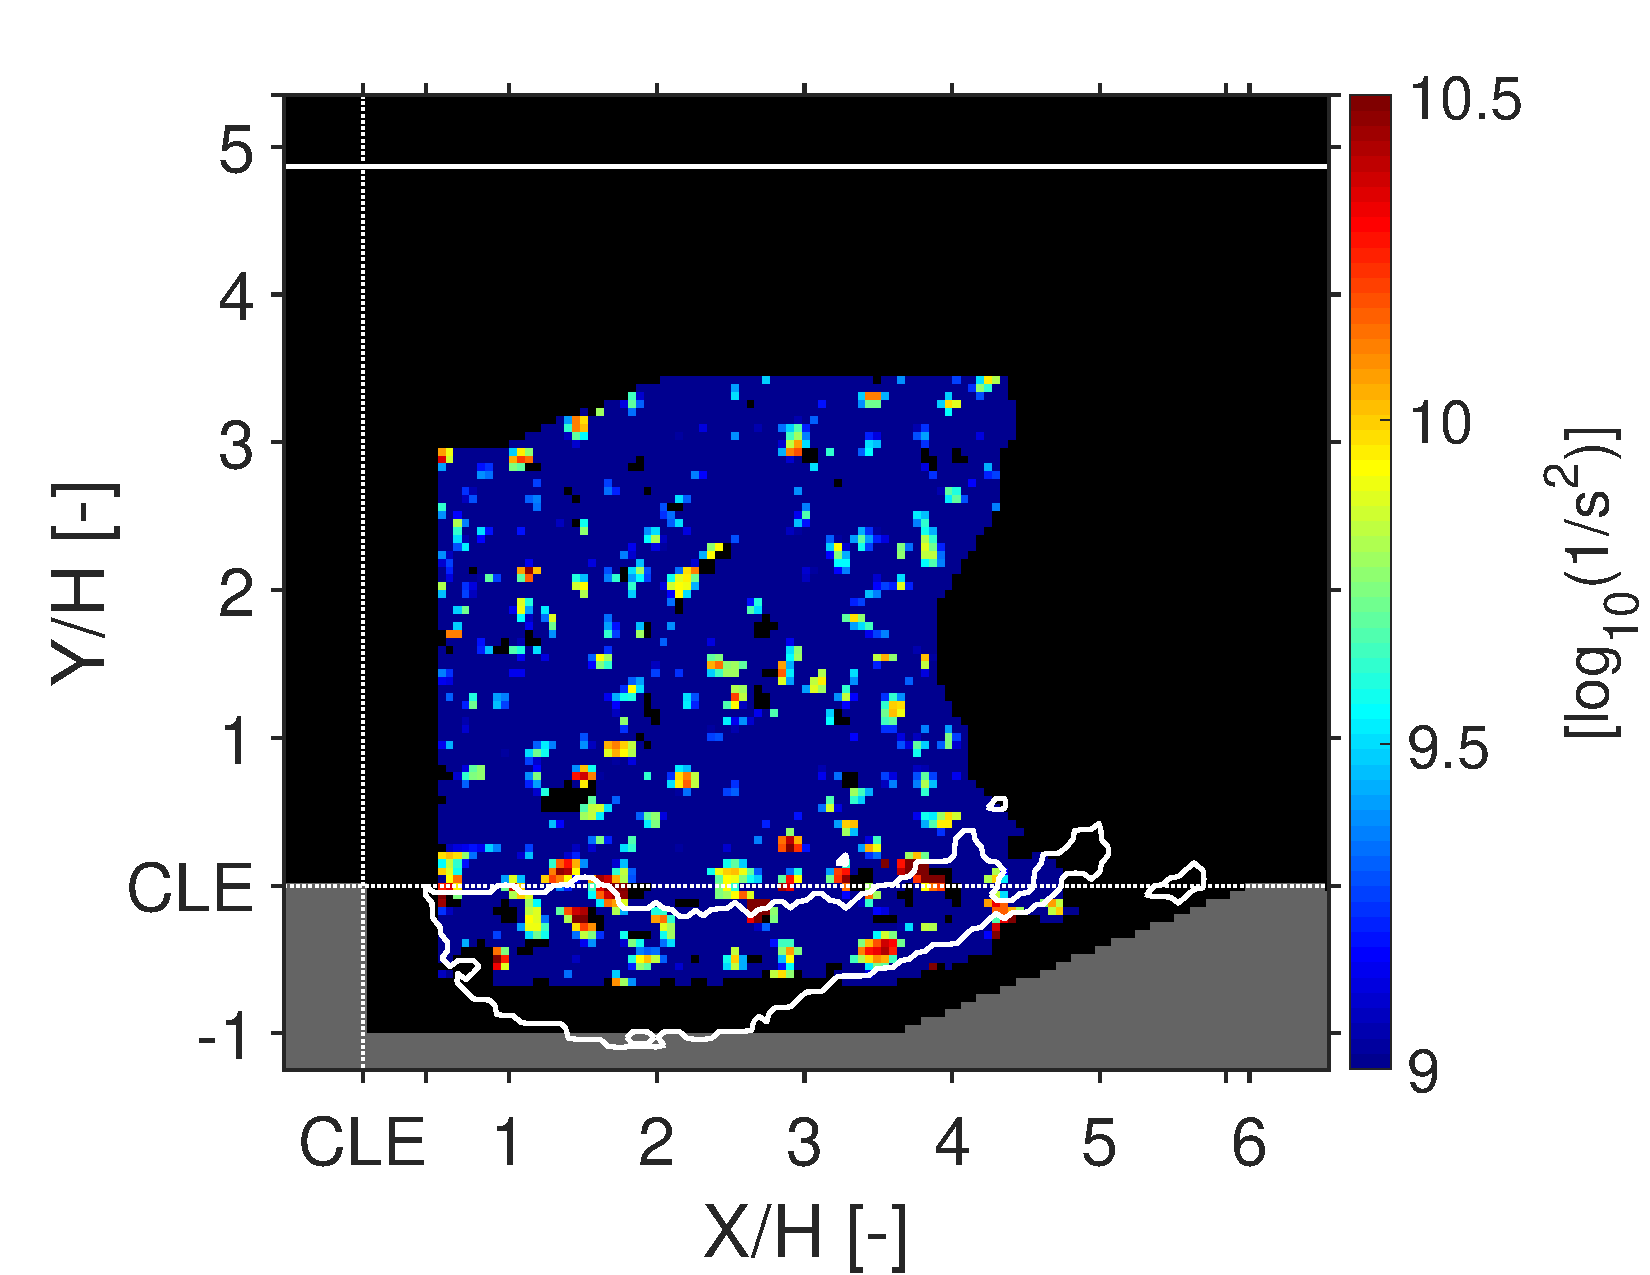
\includegraphics[width=3.25in]{figures/B1/B1_swirling_strength/B1_Frame399.pdf}} \\
\subcaptionbox{State 3\label{fig:B1_R3_ST}}{
        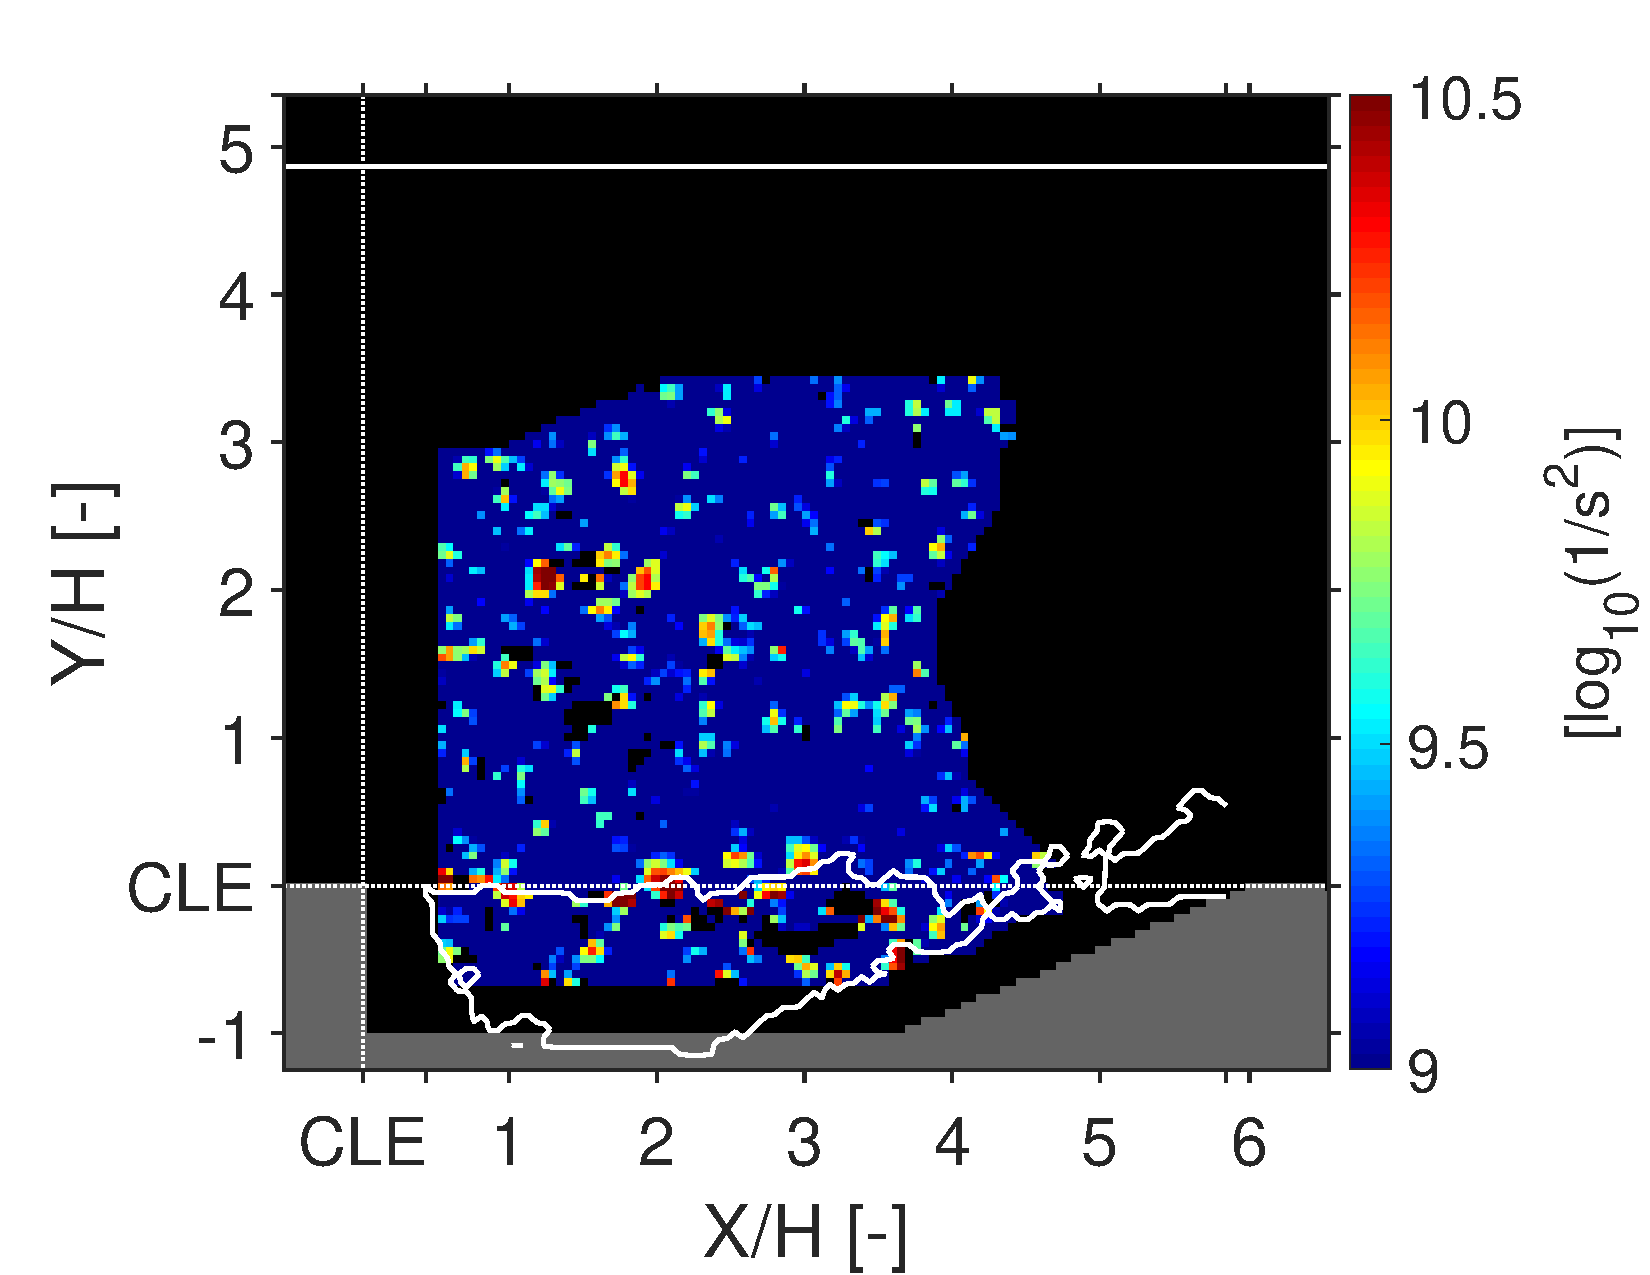
\includegraphics[width=3.25in]{figures/B1/B1_swirling_strength/B1_Frame17.pdf}}
\caption{Select instantaneous swirling strength.}
\label{fig:ch3_inst_ST}
\end{figure}

\citet{AllisonFredericksonKirikEtAl2017} demonstrated the presence of a combustion oscillation at 340 Hz in a similar dual-mode scramjet flowpath with a cavity flameholder using 50 kHz CH* chemiluminescence. These authors attributed the oscillation to thermoacoustic waves between the shock train and thermal throat. They also located the greatest variations in heat release in the region of the flame brush above the ramp. The measured 340 Hz frequency is close to the 357 Hz oscillation frequency detected in the companion LES \citep{ramesh2015large}. Evidence of a similar oscillation is observed in LES applied to the present flowpath \citep{Nielsen2019}, where periodic flame structures ejected from the cavity can also be observed. It is therefore expected that the present flow is subject to thermoacoustic oscillation between the shock train and combustion region (see \citet{MatsuoMiyazatoKim1999} and \citet{WangWangSun2014}). 

%The hypothetical cycle consists of three typical flow states: a cavity-enclosed flame (state 1), a stretched flame extending past the cavity ramp and interface (state 2), which subsequently leads to the ejection of products (state 3). This order is illustrated in Fig. \ref{fig:cycle_diagram} corresponding to the sequence of Figs. \ref{fig:B1_Frame1} to \ref{fig:B1_Frame5}. 

In state 1 (Fig. \ref{fig:B1_Frame1}), the cavity gases are contained within the cavity by the high momentum of the duct flow, leading to shear layer impingement on the cavity ramp. The cavity recirculation zone consists of two large clockwise vortices, expected to grow from the merging of smaller eddies formed at the impingement location \citep{TuttleCarterHsu2014, Kirik2017}. Mass exchange between the duct flow and the cavity flow is low as it occurs mostly through the shear layer rather than along the ramp. Generated heat is thus mostly stored in the cavity by the trapped recirculation zone. During this flow state, some heat may escape at the shear layer impingement zone along the ramp (hidden to the PIV-PLIF cameras due to setup constraints). 

State 1 is unsustainable due to the mass and heat accumulation into the cavity. The shear layer is subsequently lifted (Fig. \ref{fig:B1_Frame2}) and detaches from the cavity ramp. An open question is whether this event is triggered by reaching a threshold in the cavity pressure and gas expansion, or by large-scale flow fluctuations from e.g. shock train fluctuations. 
The lifted shear layer provides an escape route for the trapped gases (state 2). During this event, combustion radicals and products are ejected through a narrow streamtube between the ramp and the lifted shear layer.
The ejection leads to a transfer of heat and mass from the cavity to the duct while stretching the reaction front. 
The flamefront is stretched thinnest between the two large recirculation eddies, leading to breaking of the flame front and detachment of a region of combustion products (Fig. \ref{fig:B1_Frame4}). The above events constitute state 3. Transition back to state 1 occurs as the downstream eddy is convected away by the main flow (Fig. \ref{fig:B1_Frame5}). The shear layer attaches itself back to the ramp, trapping combustion products and radicals in the cavity again. The pressure rise at the reattachment point may shift the upstream eddy towards the cavity leading edge, and a new eddy is formed from the merging of eddies created at the impingement area as suggested by \cite{TuttleCarterHsu2014}. Alternatively, a new eddy may be formed near the cavity leading edge. In this case, the upstream eddy from the previous cycle becomes the new downstream eddy. The proposed cycle is diagrammed in Fig. \ref{fig:cycle_diagram}. 

\begin{figure}
\centering
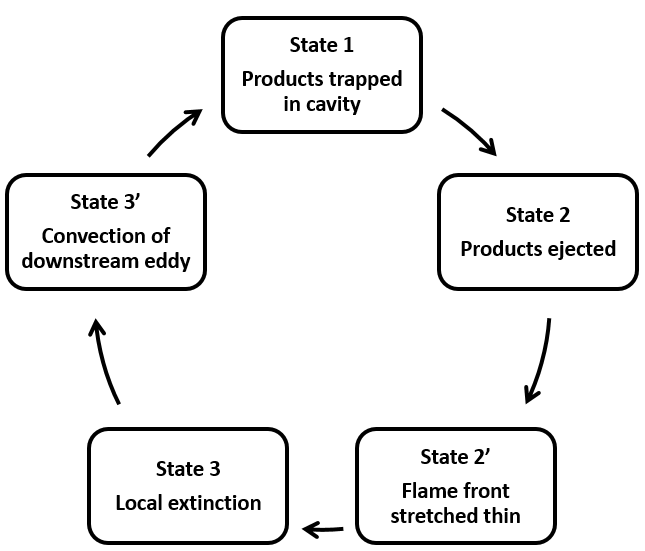
\includegraphics[width=3.25in]{figures/cycle_diagram.png}
\caption{Diagram of the hypothetical combustion cycle.}
\label{fig:cycle_diagram}
\end{figure}

The presence of both positive and negative velocity fluctuations $U'=U-U_{AVG}$ for a same phase, e.g. phase 2 in Fig. \ref{fig:B1_Frame6} versus \ref{fig:B1_Frame2}, suggests a repetition of the cavity combustion cycle within one shock train cycle. Further investigations with high-frequency pressure measurements and LES are warranted to explore the driving factors for the observed cavity combustion oscillation. 